\documentclass[11pt]{article}

\usepackage{latexsym}
\usepackage{amsmath}
\usepackage{amssymb}
\usepackage{amsthm}
\usepackage{graphicx}
\usepackage{wrapfig}
\usepackage{pseudocode}
\usepackage{url}
\usepackage[backref, colorlinks=true, citecolor=red, urlcolor=blue, pdfauthor={Jyh-Ming Lien}]{hyperref}
\usepackage{subfigure}


\newcommand{\handout}[5]{
  \noindent
  \begin{center}
  \framebox{
    \vbox{
      \hbox to 5.78in { {\bf } \hfill #2 }
      \vspace{4mm}
      \hbox to 5.78in { {\Large \hfill #5  \hfill} }
      \vspace{2mm}
      \hbox to 5.78in { {\em #3 \hfill #4} }
    }
  }
  \end{center}
  \vspace*{4mm}
}

\newcommand{\lecture}[4]{\handout{#1}{#2}{#3}{}{Report for #1}}

\newtheorem{theorem}{Theorem}
\newtheorem{corollary}[theorem]{Corollary}
\newtheorem{lemma}[theorem]{Lemma}
\newtheorem{observation}[theorem]{Observation}
\newtheorem{proposition}[theorem]{Proposition}
\newtheorem{definition}[theorem]{Definition}
\newtheorem{claim}[theorem]{Claim}
\newtheorem{fact}[theorem]{Fact}
\newtheorem{assumption}[theorem]{Assumption}

% 1-inch margins, from fullpage.sty by H.Partl, Version 2, Dec. 15, 1988.
\topmargin 0pt
\advance \topmargin by -\headheight
\advance \topmargin by -\headsep
\textheight 8.9in
\oddsidemargin 0pt
\evensidemargin \oddsidemargin
\marginparwidth 0.5in
\textwidth 6.5in

\parindent 0in
\parskip 1.5ex
%\renewcommand{\baselinestretch}{1.25}

\begin{document}

\lecture{Advance Algorithm Programming Assignment 1 }{Fall 2015}{Yeojin Kim}{---}


\section{Implementation Details}
\subsection{algorithm}
The algorithm is as follows:
\begin{enumerate}
\item Create points in 4D using 3 coordinates : $\mathbf{(x,y, z, x^2+y^2+z^2)}$
\item Compute convex hull in 4D by calling qhull\cite{Qhull} with 4D points.
\item Looping through all facets in 4D convex hull,
\subitem - Save the vertices of a facets as the vertices of tetrahedron. This vertices are 3 coordinates$\mathbf{(x,y,z)}$.
\subitem - Compute the sign volume of tetrahedron
\subitem - If the normal vector of tetrahedron points downward and the volume is not zero, generate faces of tetrahedron. In other words, if this tetrahedron is lower convex hull and all points are not coplanar, render this tetrahedron.
\end{enumerate}
\subsection{software}
OS : Window 8.1K\\
IDE : Visual Studio 2013\\
*NOTE :  I use the dynamic library for freeglut.

\section{Example Output}
 Here are example results. Each image in Fig. \ref{fig:cube} ~ Fig. \ref{fig:teeth} shows that (a) A set of points, (b) a set of edges in Delanauy triangulation, (c)a set of faces in Delanauy triangulation, and (d) a set of total tetrahedra. We can observe that Delanauy triangulation does not have intersections between edges. Otherwise, a simple projection of whole tetrahedra has multiple intersections between edges (Fig. \ref{fig:T}).
\begin{figure*}[hbt]
 \centering
  \subfigure[]{
    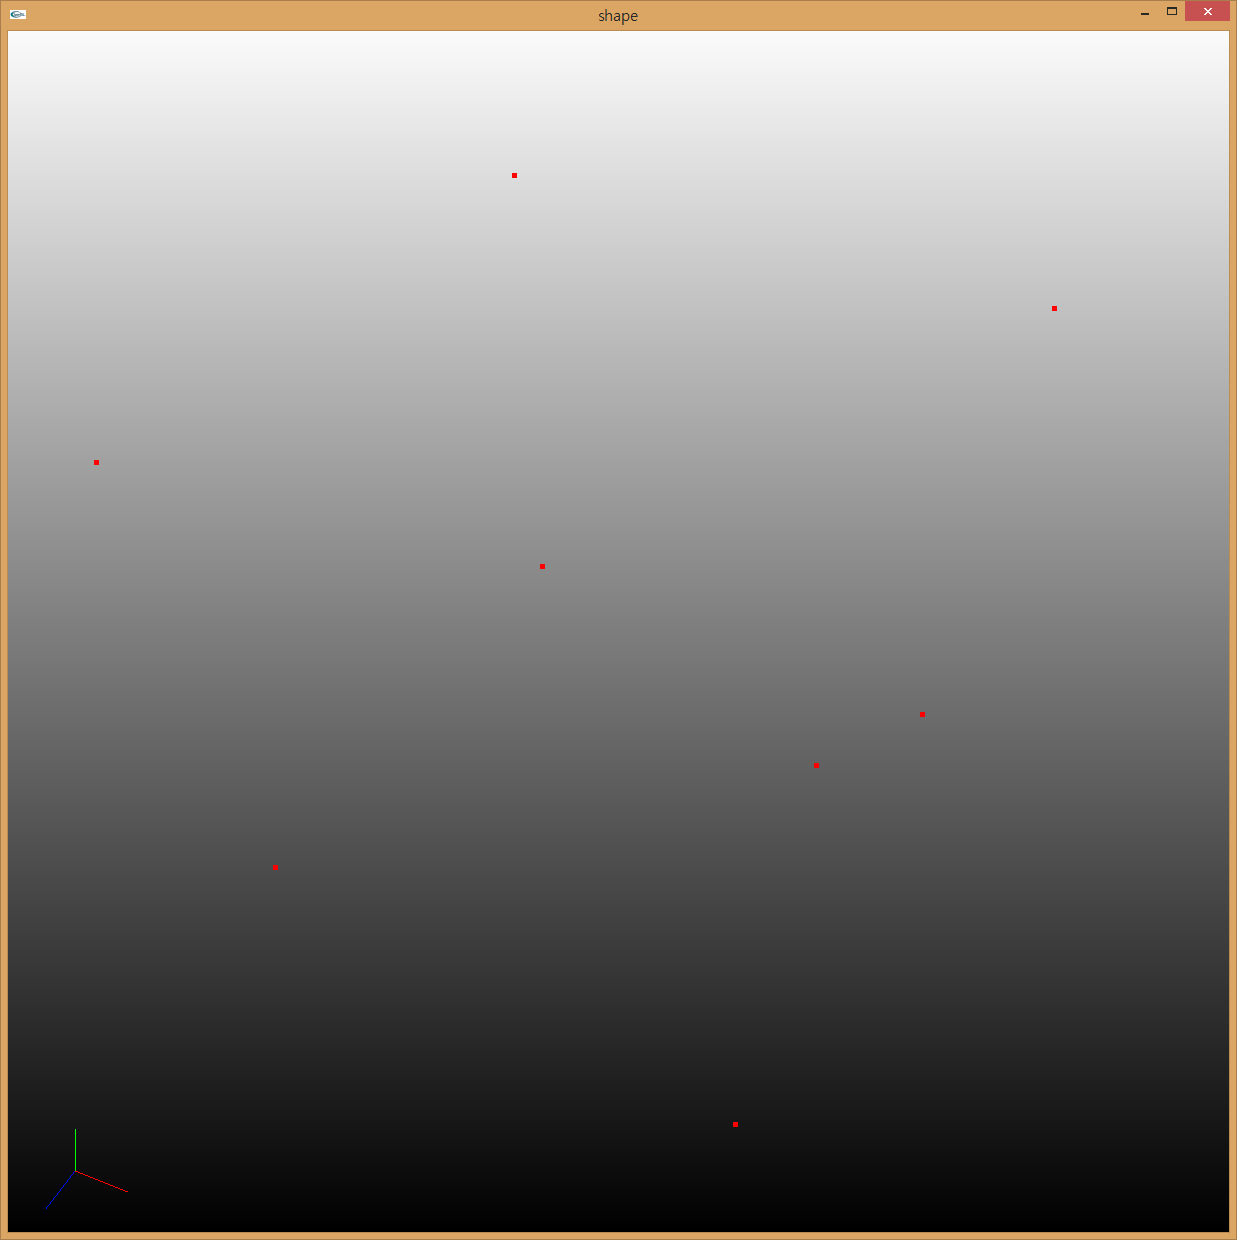
\includegraphics[width=0.22\textwidth]{img/cube3.png}
    \label{fig:cubeOption3}
  }\hspace{-3mm}
  \subfigure[]{
     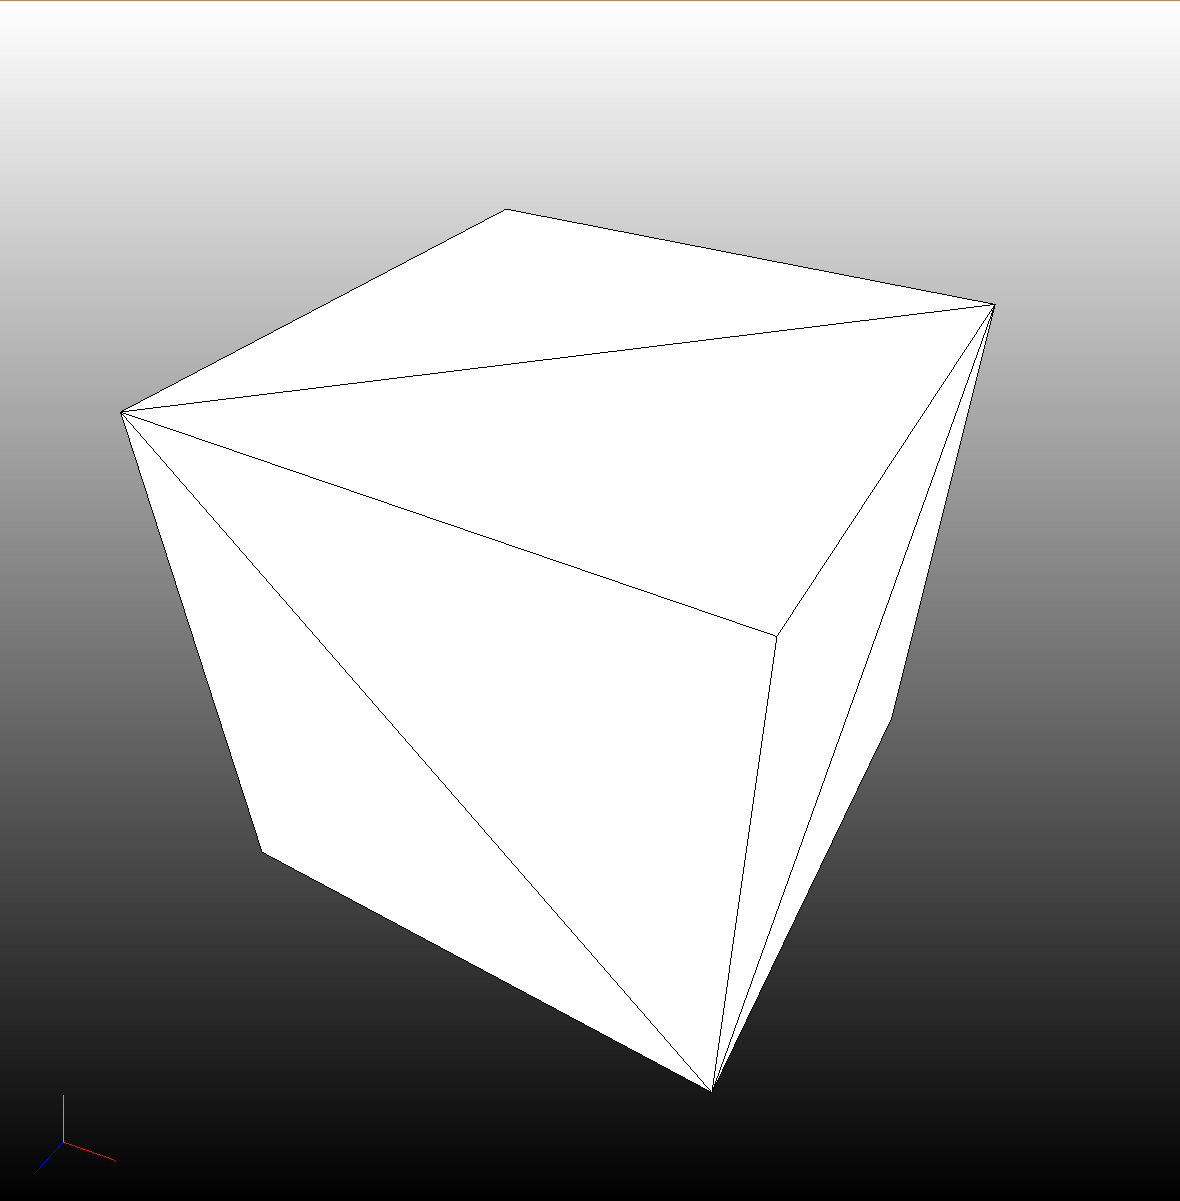
\includegraphics[width=0.22\textwidth]{img/cube2.png}
     \label{fig:cubeOption2}
  }\hspace{-3mm}
  \subfigure[]{
    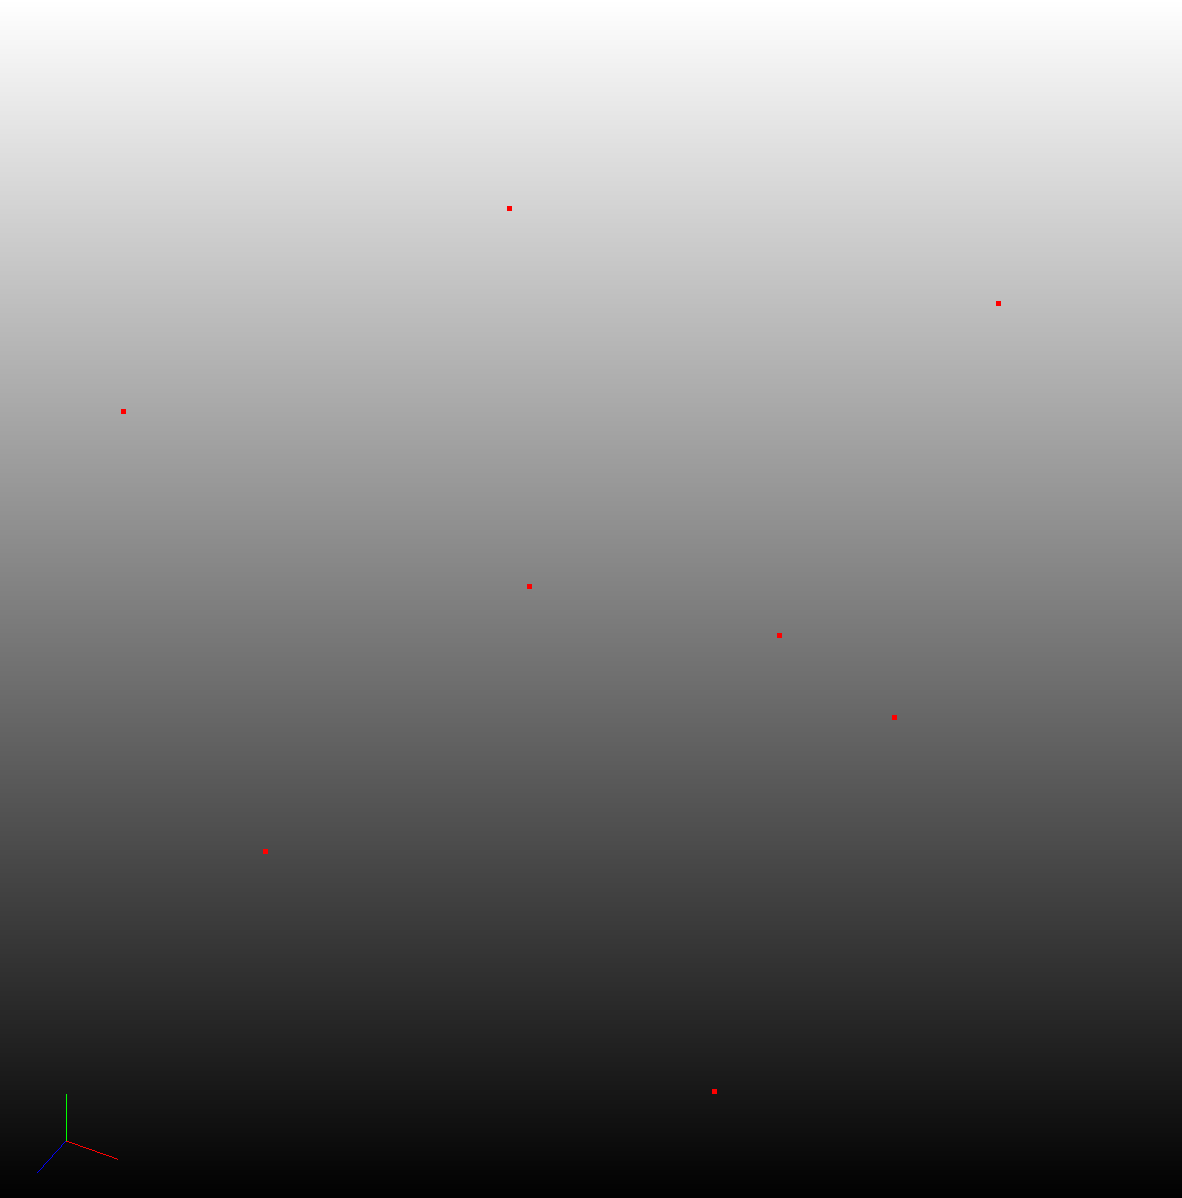
\includegraphics[width=0.22\textwidth]{img/cube1.png}
     \label{fig:cubeOption1}
  }\hspace{-3mm}
 \subfigure[]{
   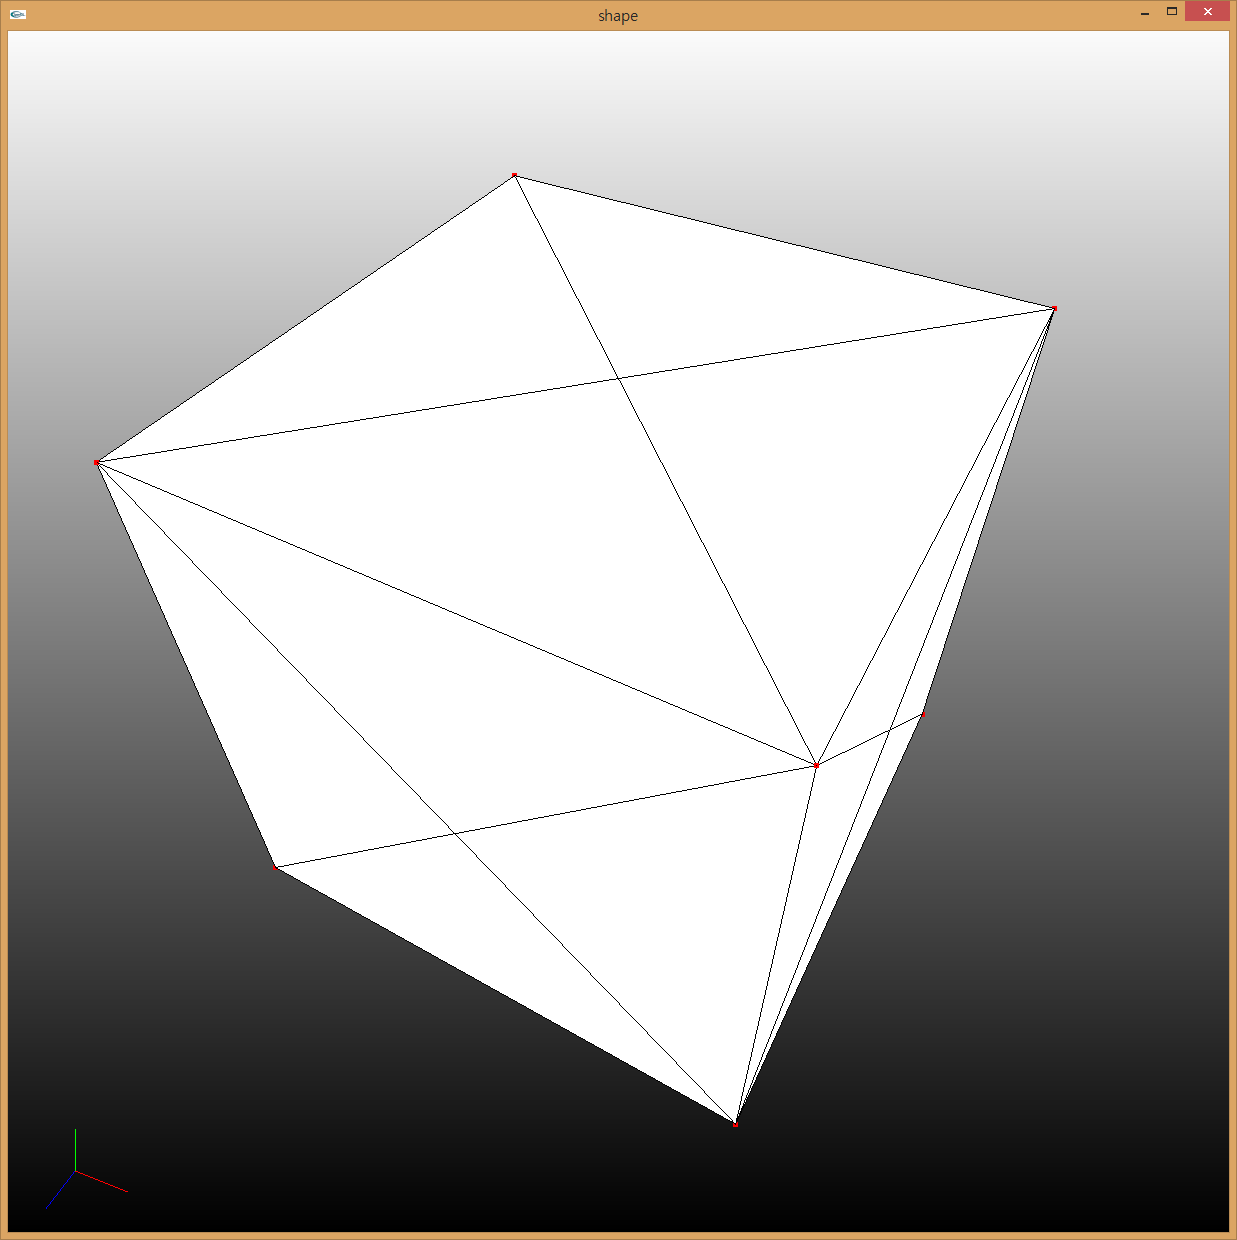
\includegraphics[width=0.22\textwidth]{img/cube4.png}
    \label{fig:cubeOption4}
 }\hspace{-3mm}
   \caption{A cube example\label{fig:cube}}
\end{figure*}
\begin{figure*}[hbt]
 \centering
  \subfigure[]{
    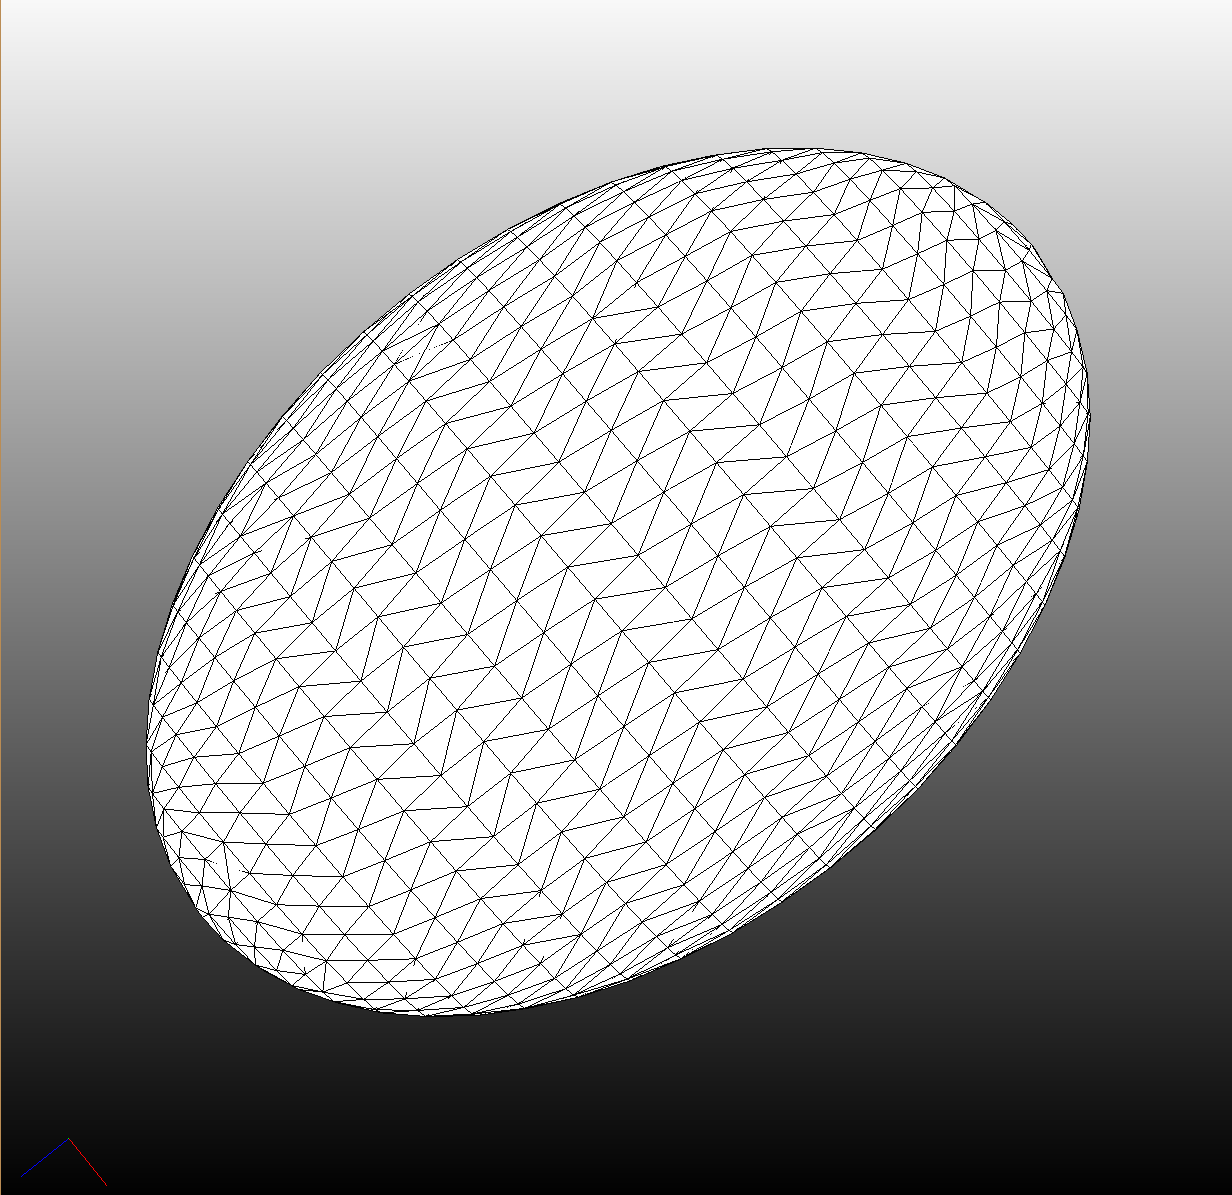
\includegraphics[width=0.22\textwidth]{img/ellipsoid3.png}
    \label{fig:ellipsoidOption3}
  }\hspace{-3mm}
  \subfigure[]{
     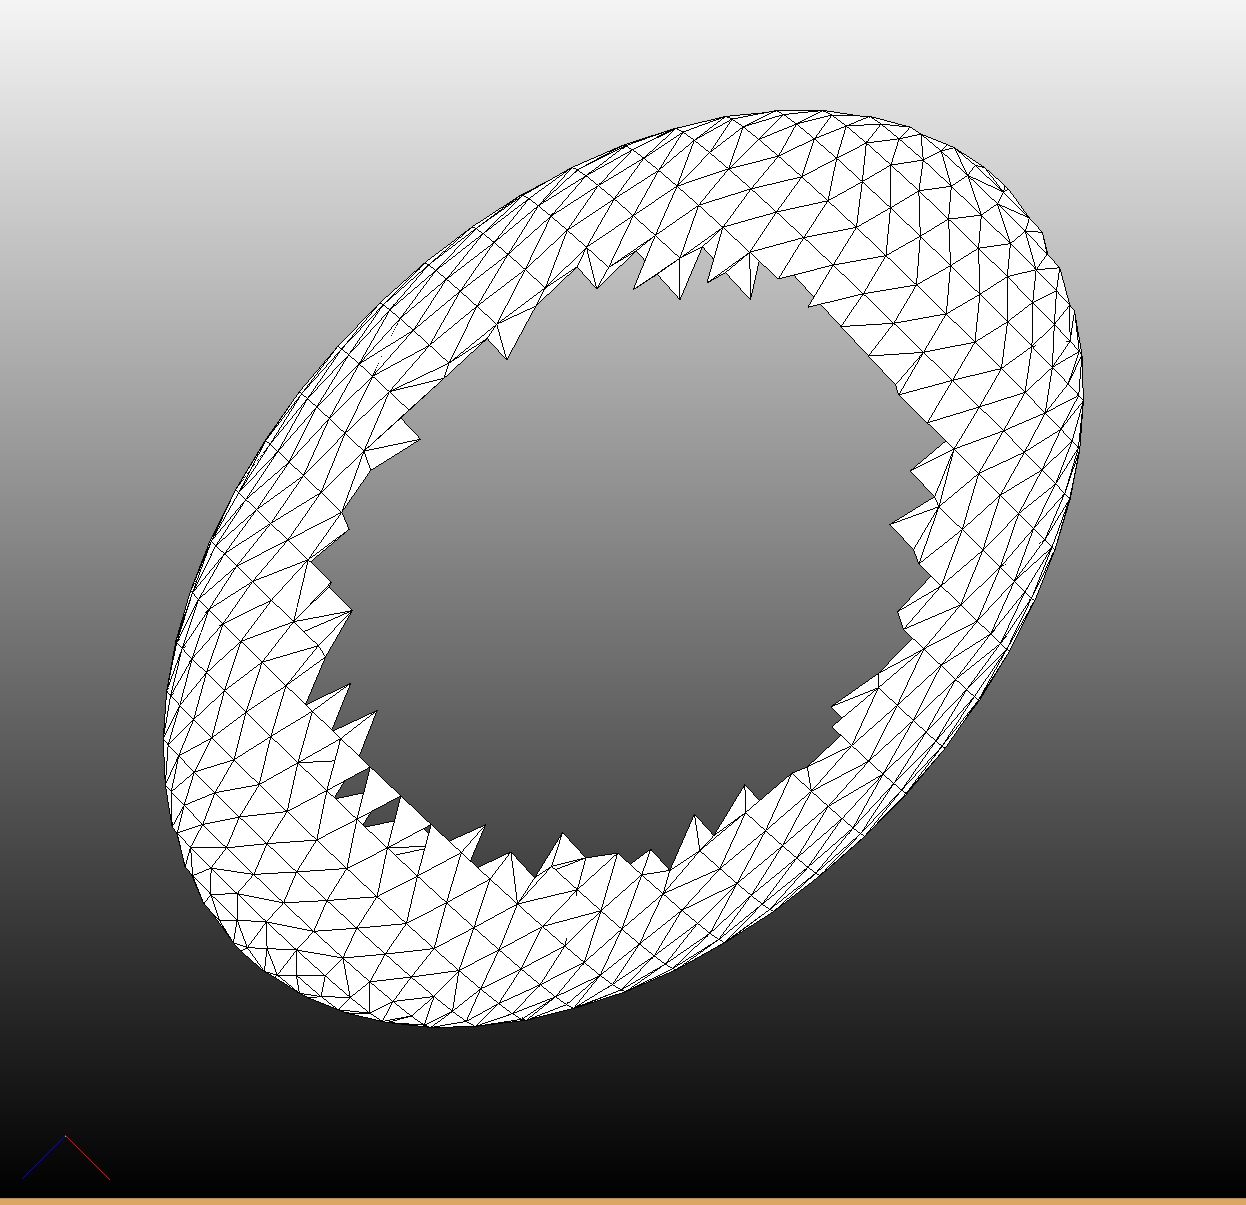
\includegraphics[width=0.22\textwidth]{img/ellipsoid2.png}
     \label{fig:ellipsoidOption2}
  }\hspace{-3mm}
  \subfigure[]{
    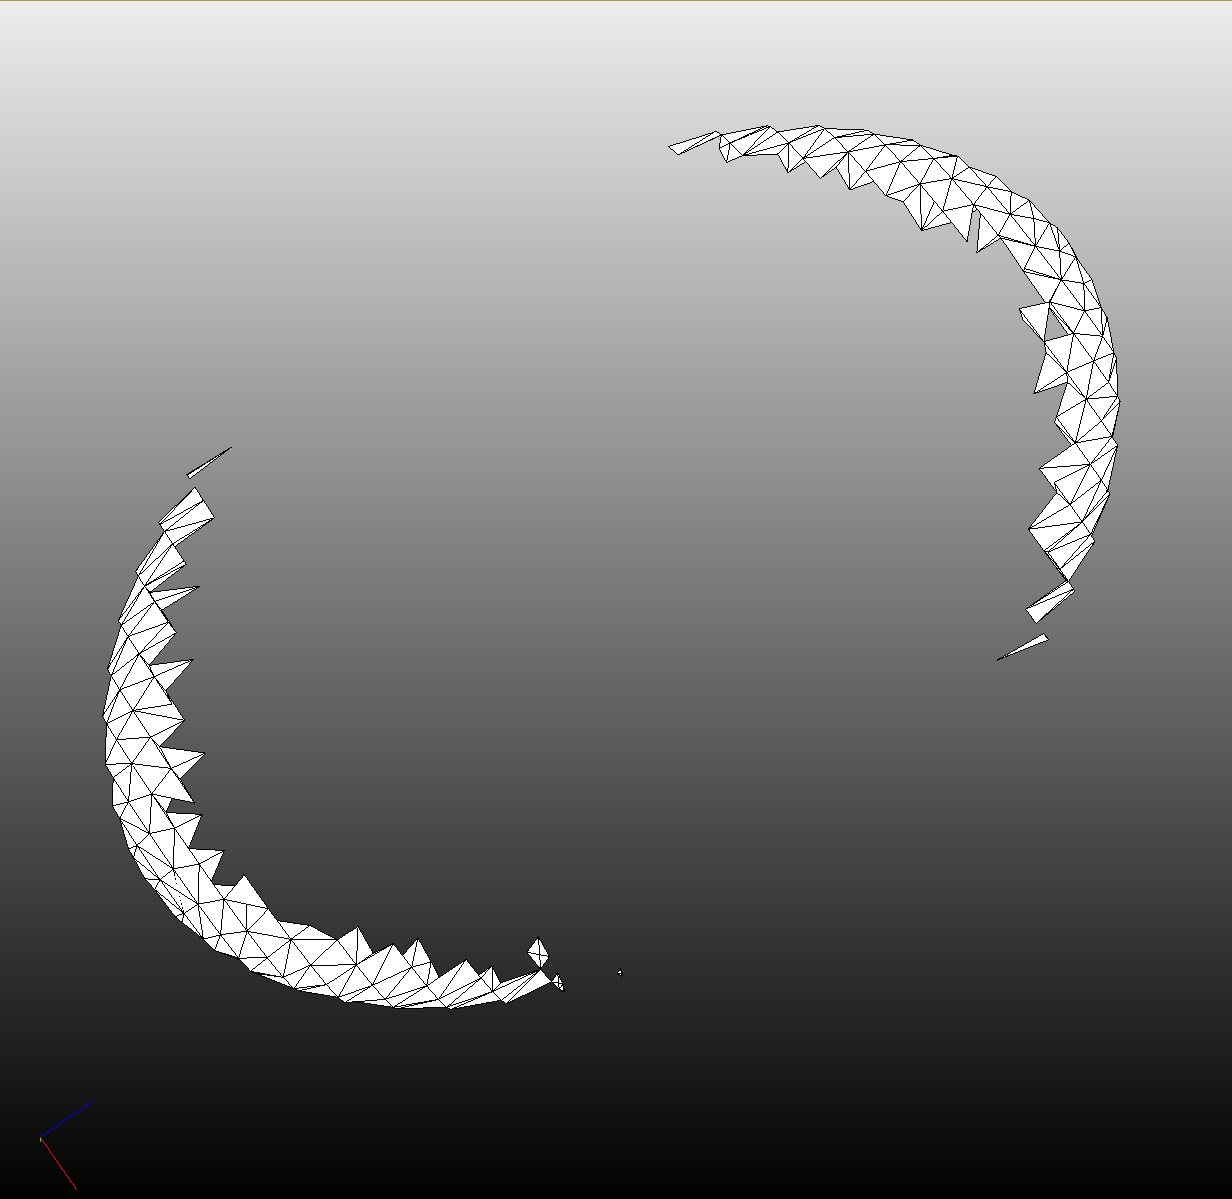
\includegraphics[width=0.22\textwidth]{img/ellipsoid1.png}
     \label{fig:ellipsoidOption1}
  }\hspace{-3mm}
  \subfigure[]{
    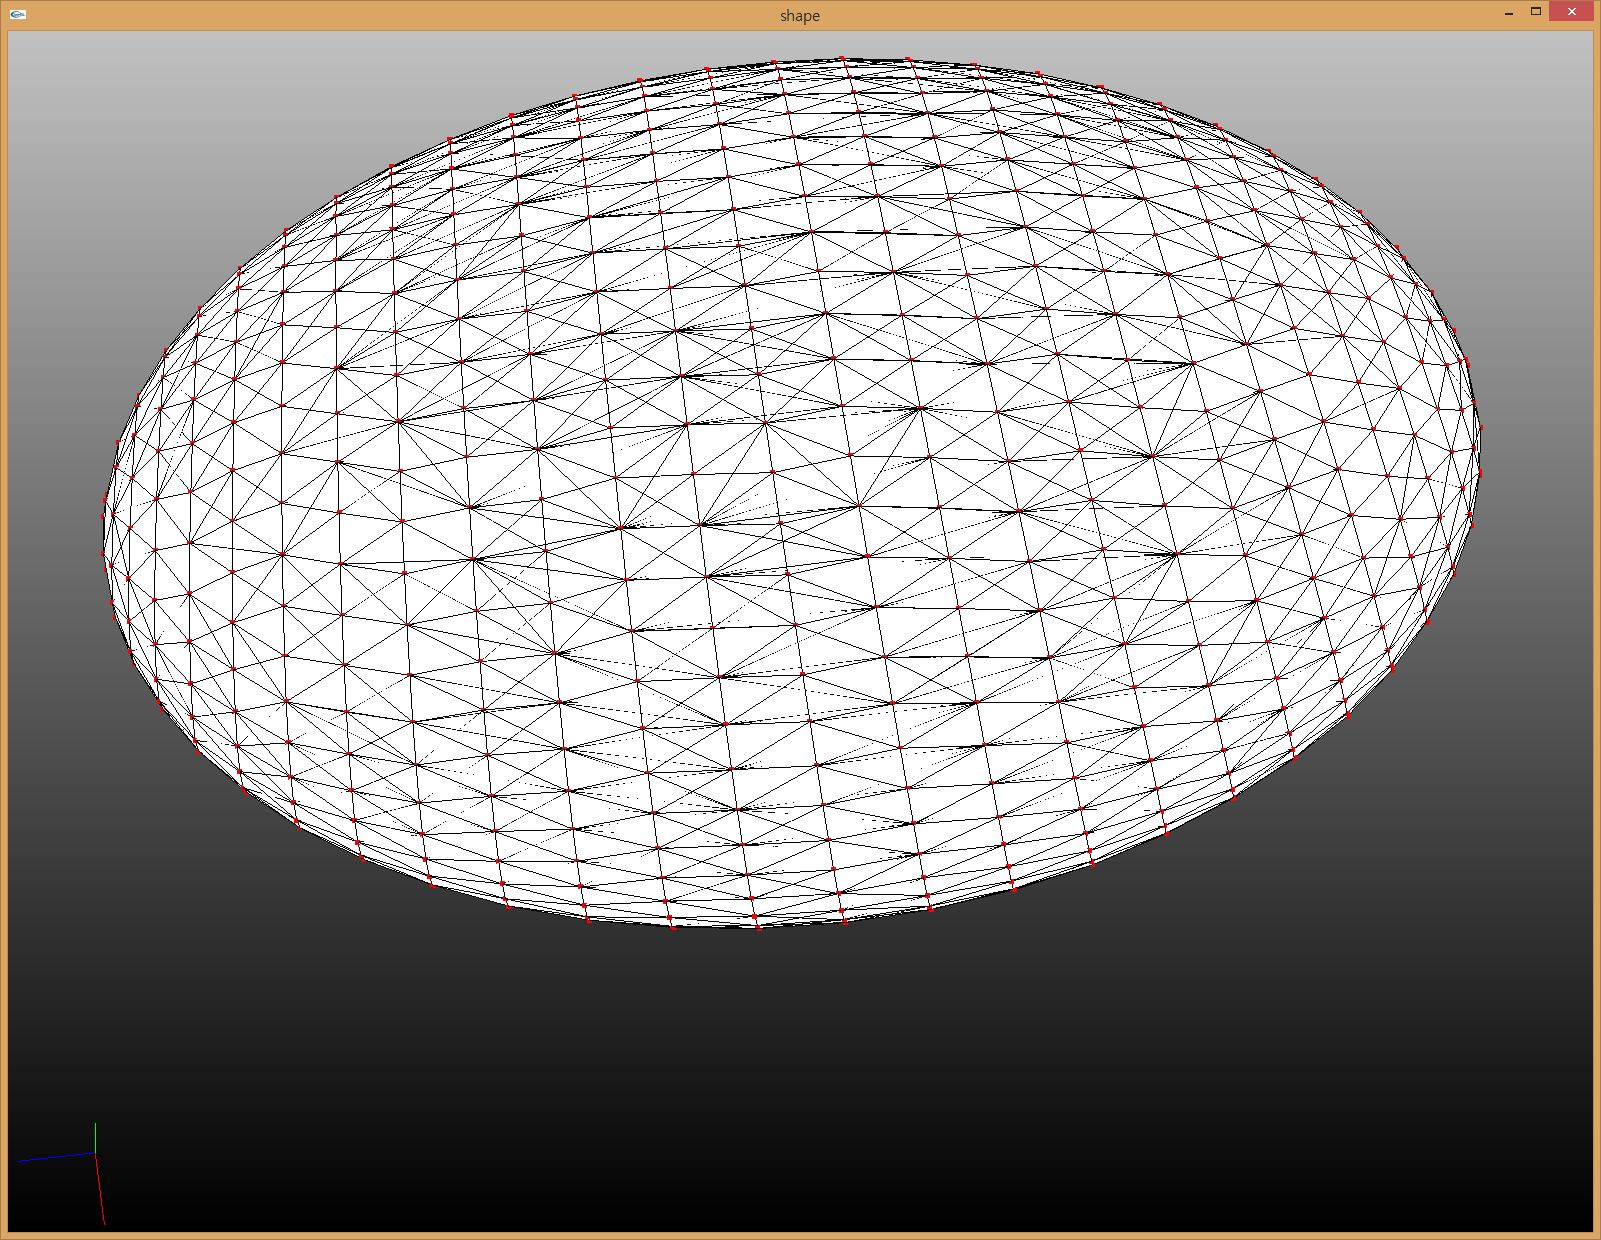
\includegraphics[width=0.22\textwidth]{img/ellipsoid4.png}
     \label{fig:ellipsoidOption4}
  }\hspace{-3mm}
  \caption{An ellipsoid example \label{fig:ellipsoid}}
\end{figure*}
\begin{figure*}[hbt]
 \centering
  \subfigure[]{
    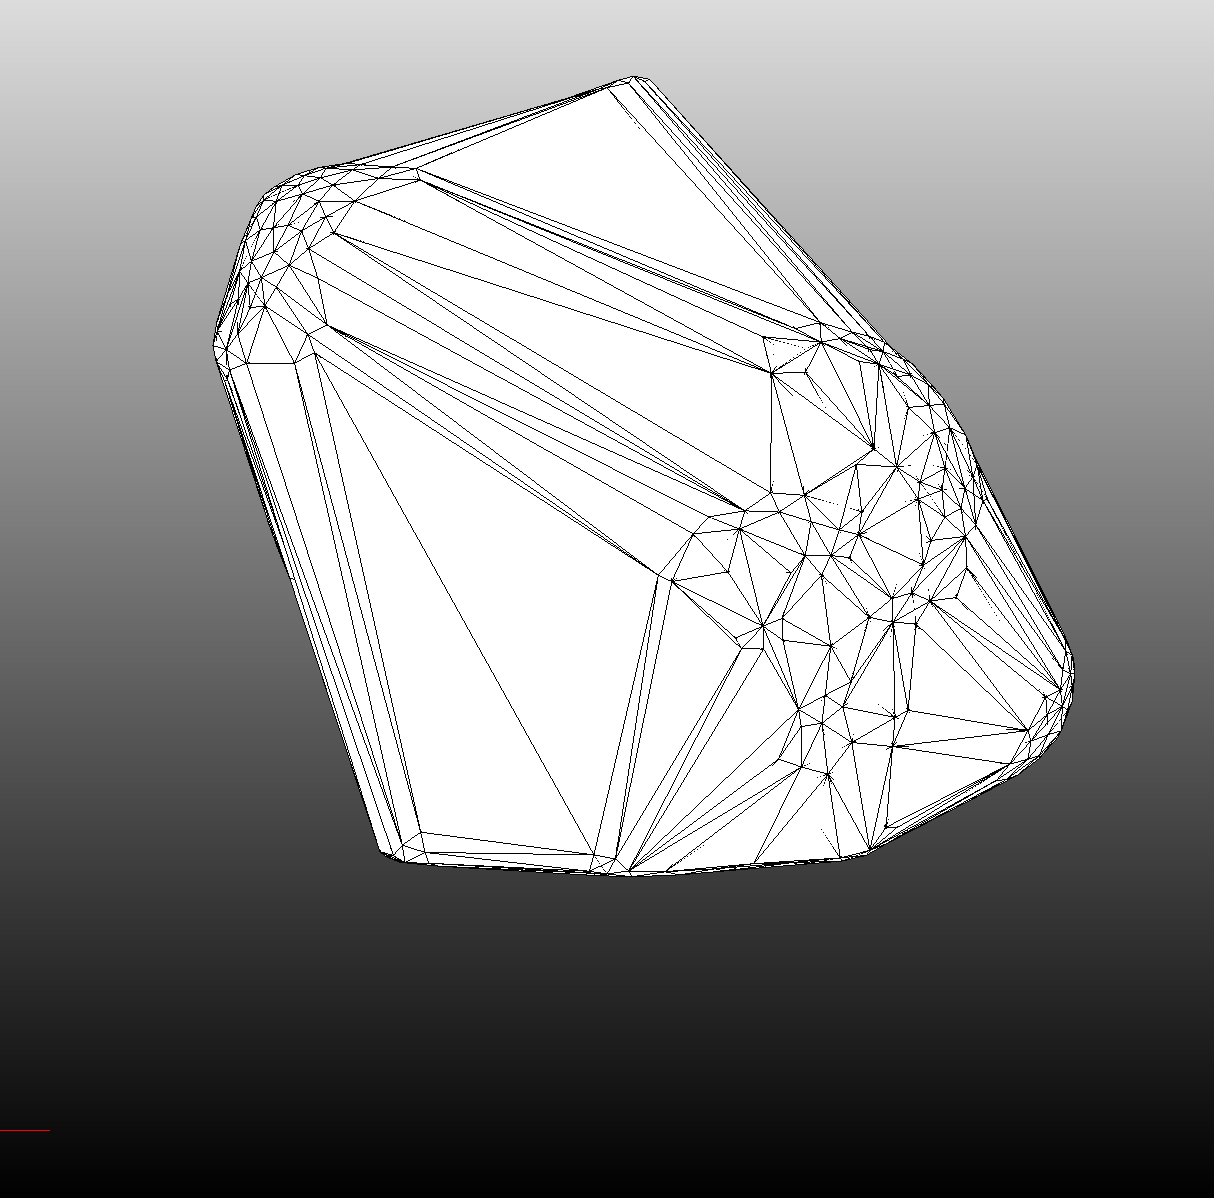
\includegraphics[width=0.22\textwidth]{img/bunny3.png}
    \label{fig:bunnyOption3}
  }\hspace{-3mm}
  \subfigure[]{
     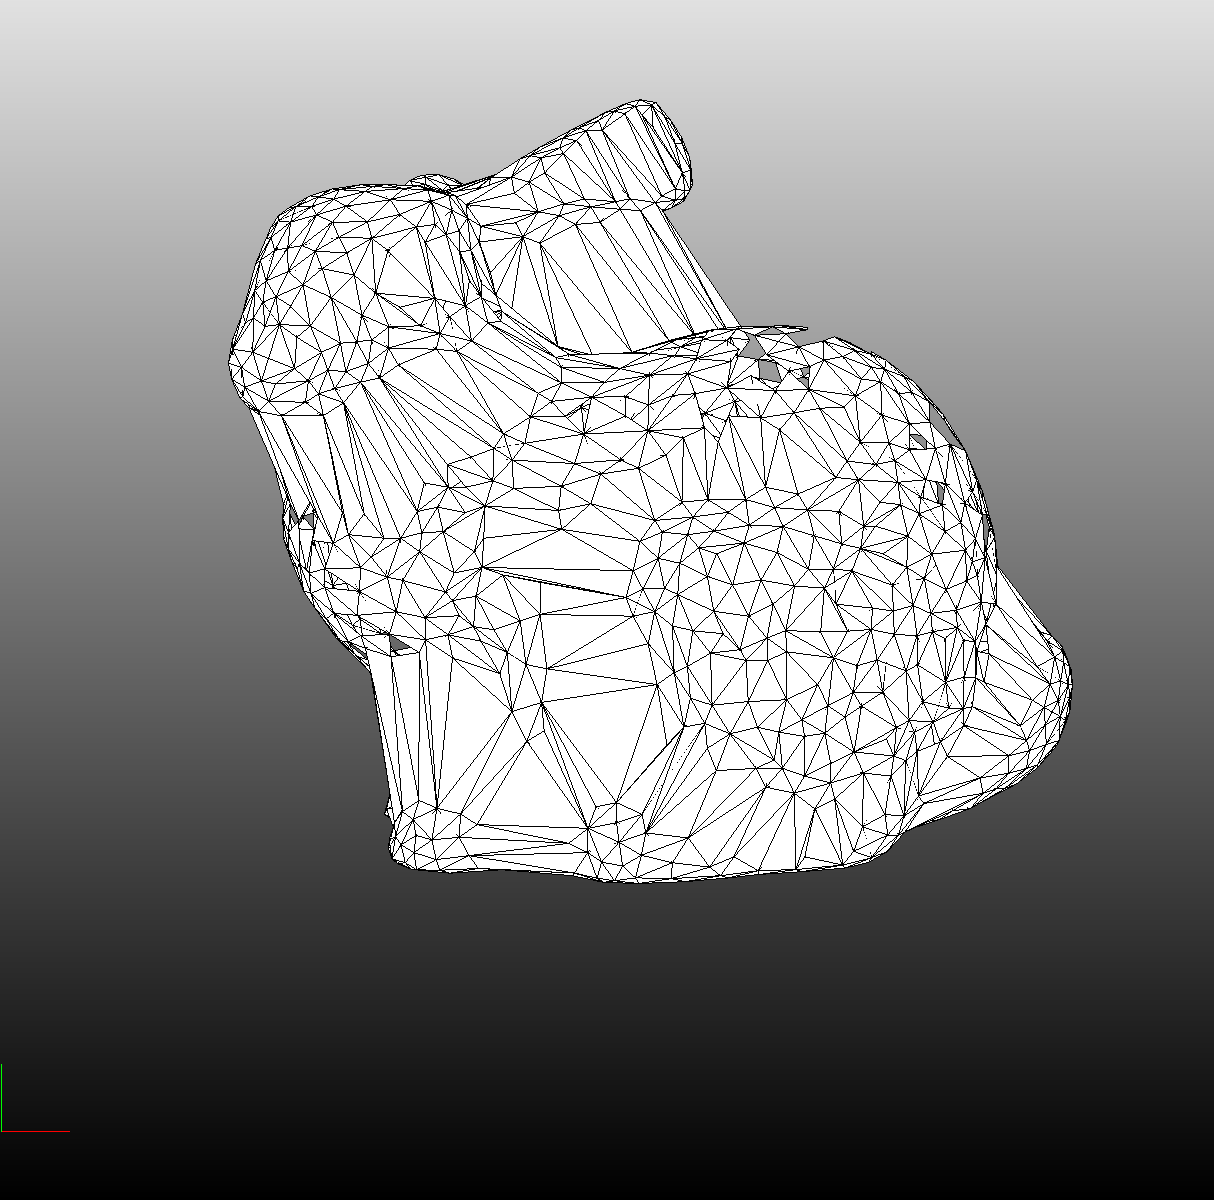
\includegraphics[width=0.22\textwidth]{img/bunny2.png}
     \label{fig:bunnyOption2}
  }\hspace{-3mm}
  \subfigure[]{
    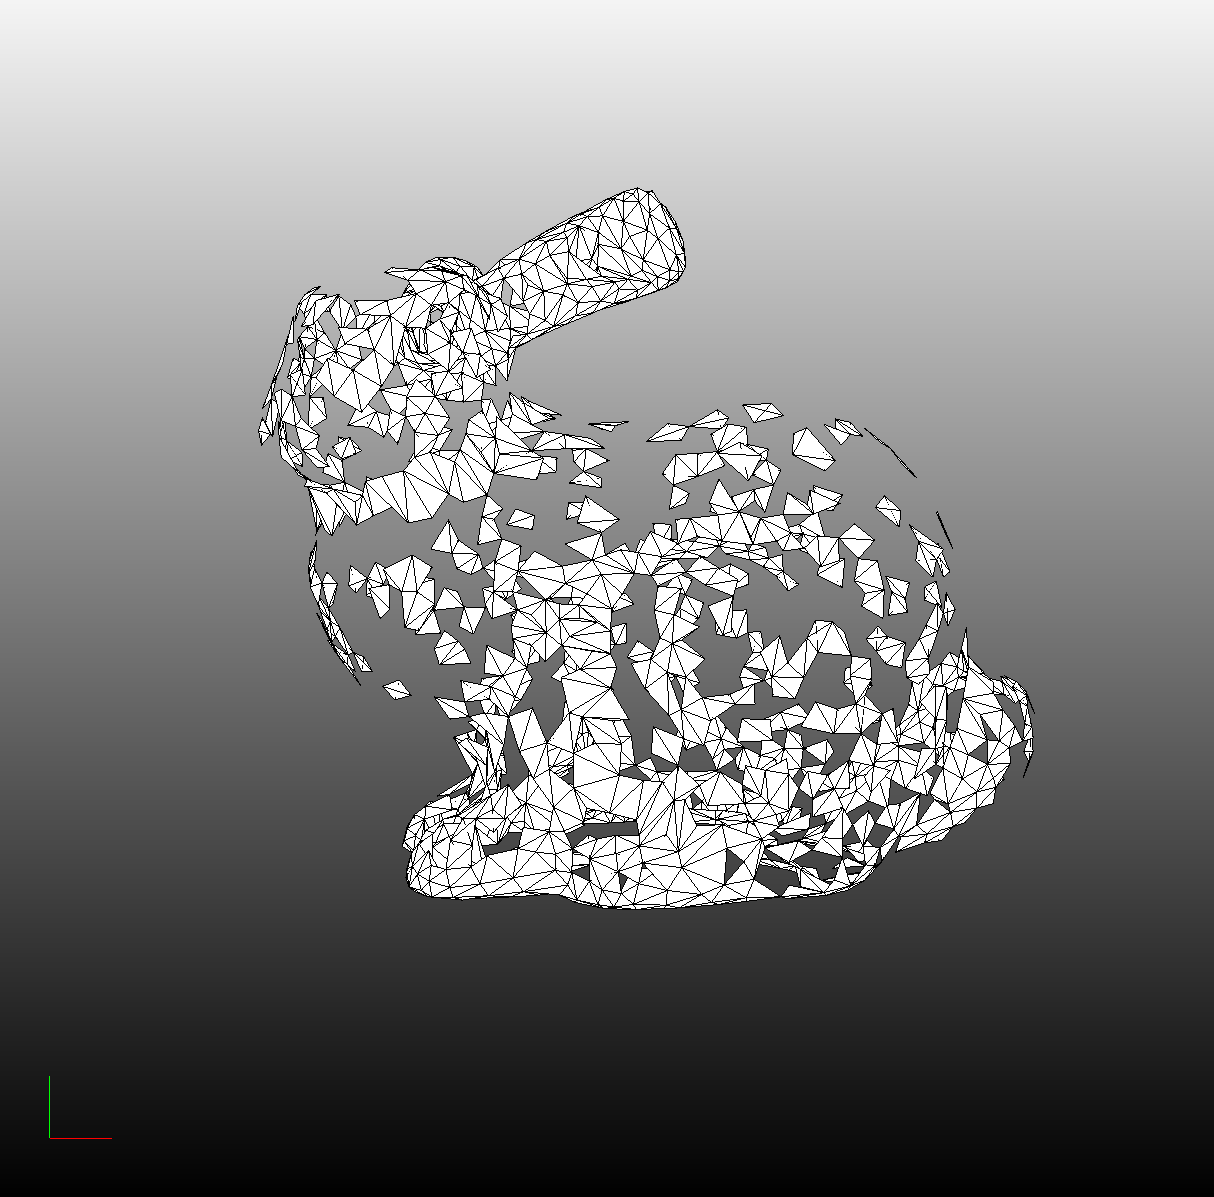
\includegraphics[width=0.22\textwidth]{img/bunny1.png}
     \label{fig:bunnyOption1}
  }\hspace{-3mm}
  \subfigure[]{
    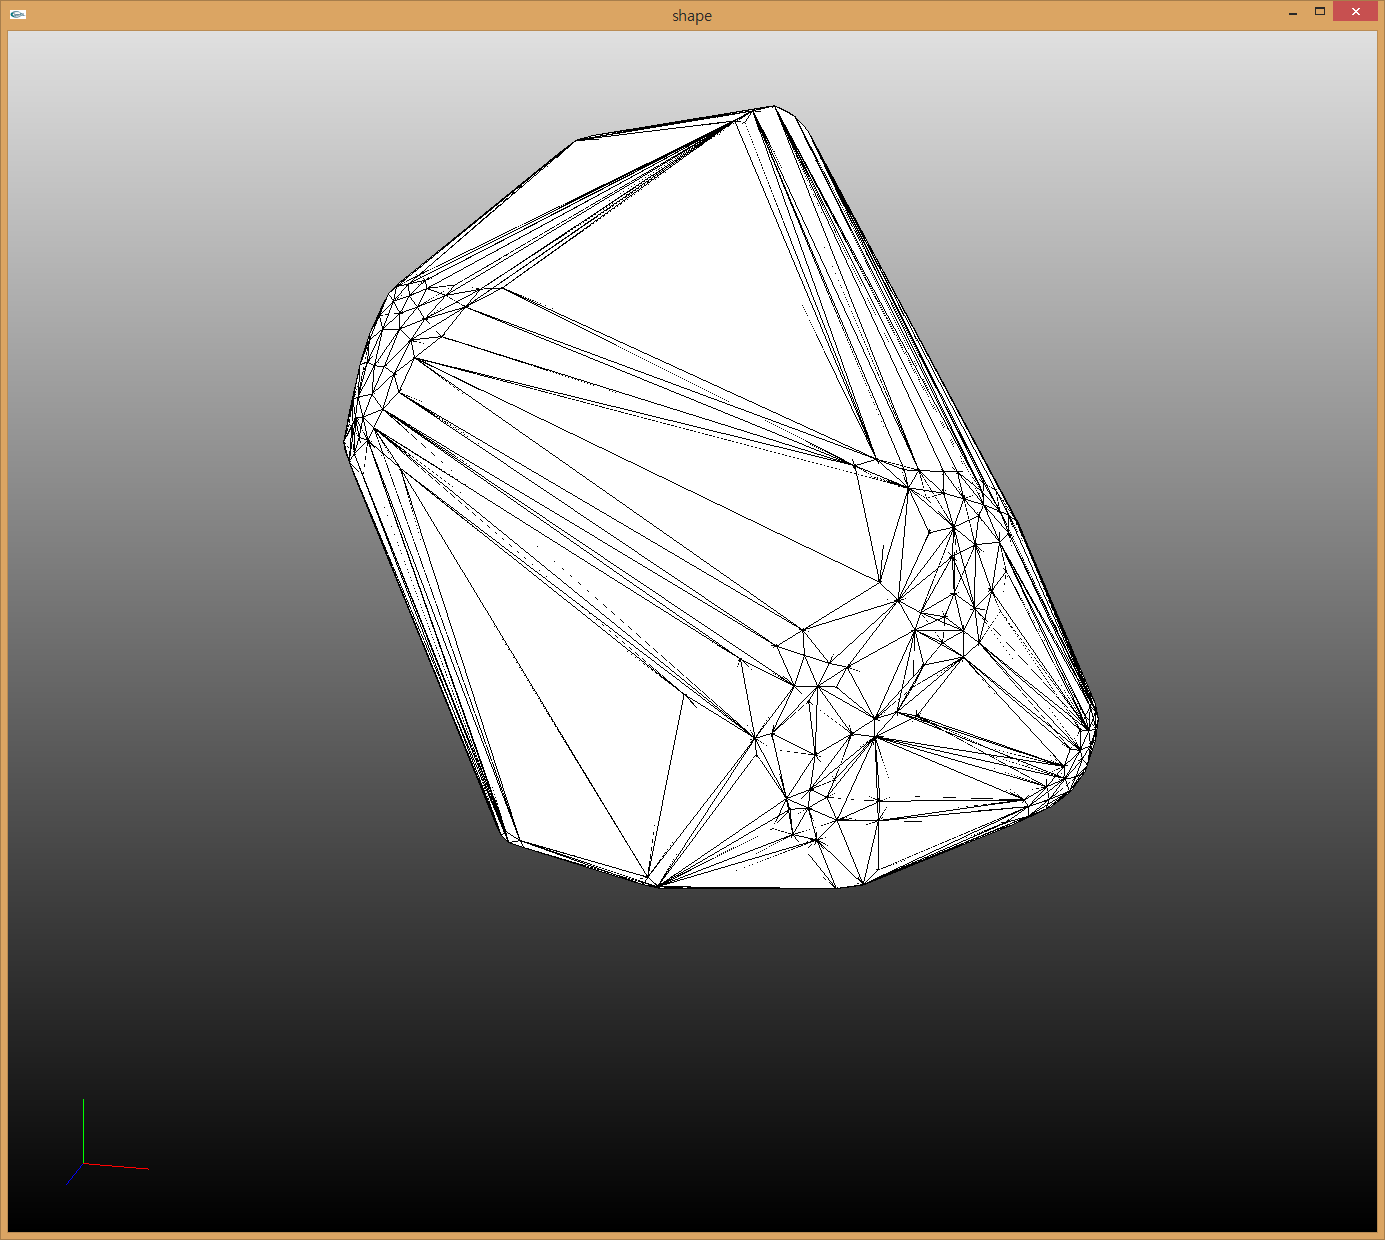
\includegraphics[width=0.22\textwidth]{img/bunny4.png}
     \label{fig:bunnyOption4}
  }\hspace{-3mm}
  \caption{A bunny example \label{fig:bunny}}
\end{figure*}
\begin{figure*}[hbt]
 \centering
  \subfigure[]{
    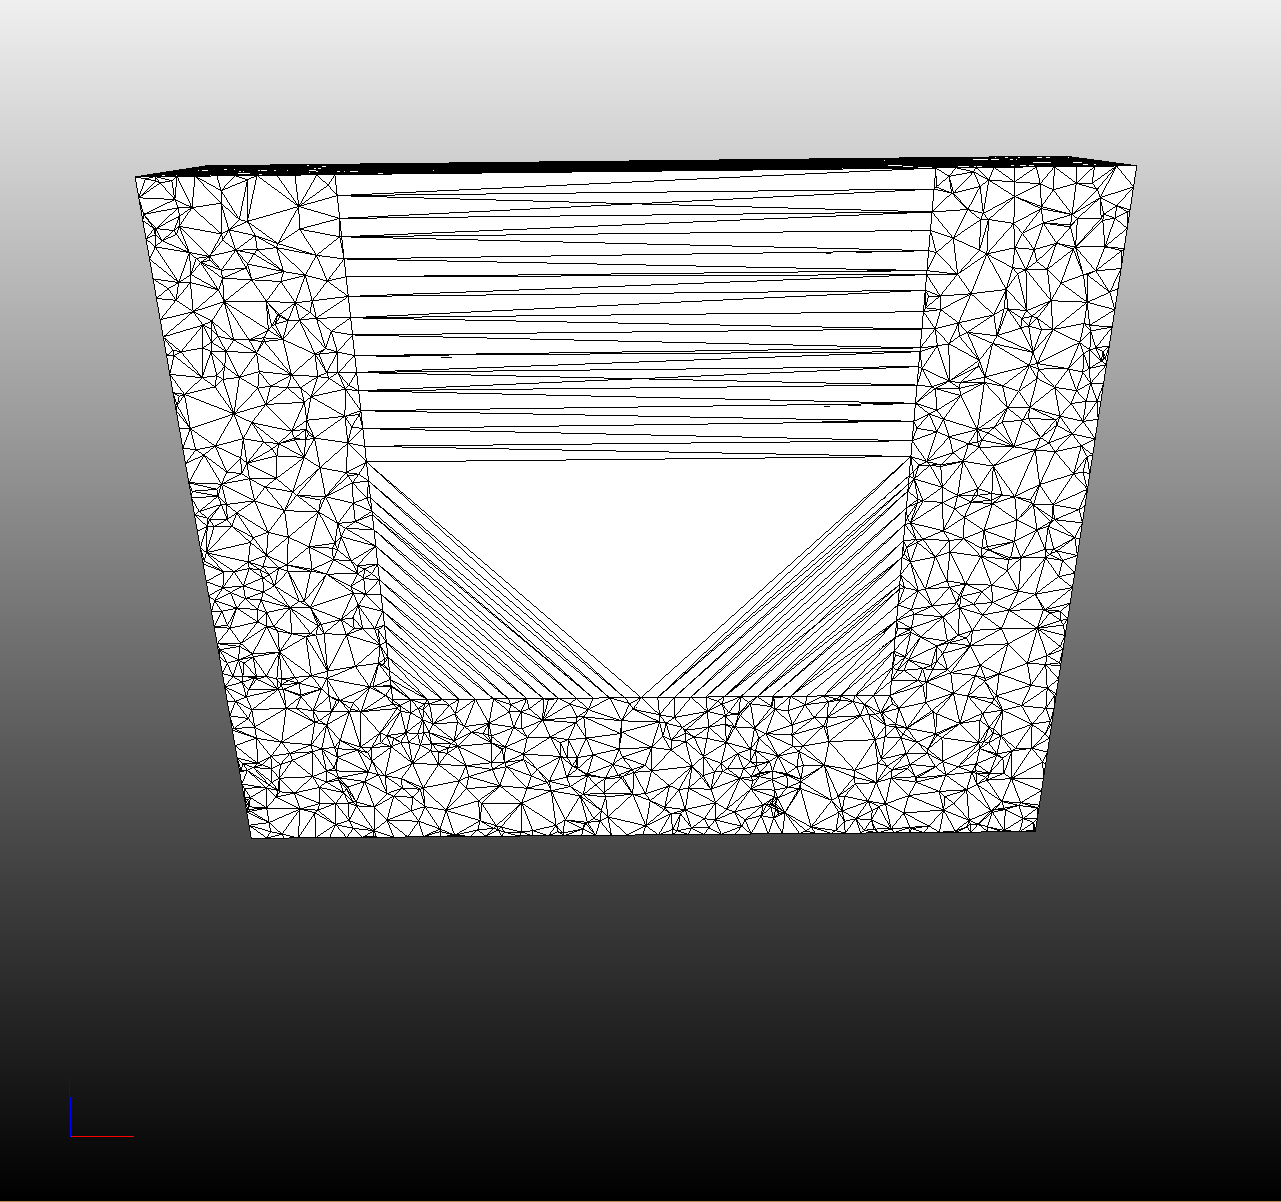
\includegraphics[width=0.22\textwidth]{img/U3.png}
    \label{fig:uOption3}
  }\hspace{-3mm}
  \subfigure[]{
     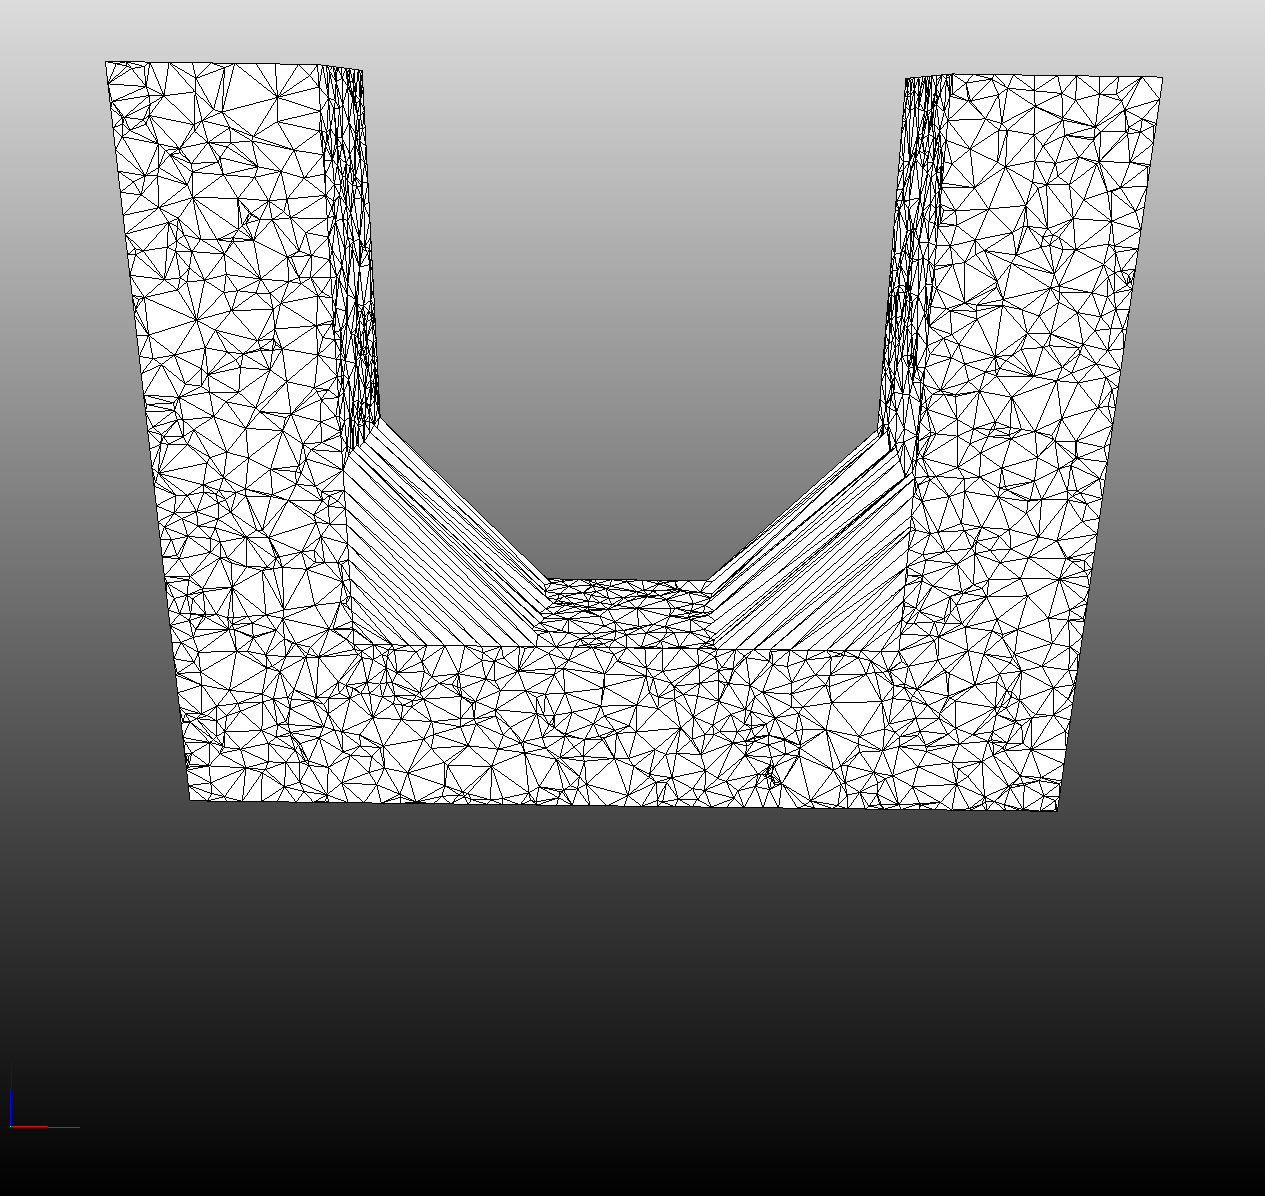
\includegraphics[width=0.22\textwidth]{img/U2.png}
     \label{fig:uOption2}
  }\hspace{-3mm}
  \subfigure[]{
    
\includegraphics[width=0.22\textwidth]{img/U1.png}
     \label{fig:uOption1}
  }\hspace{-3mm}
  \subfigure[]{
    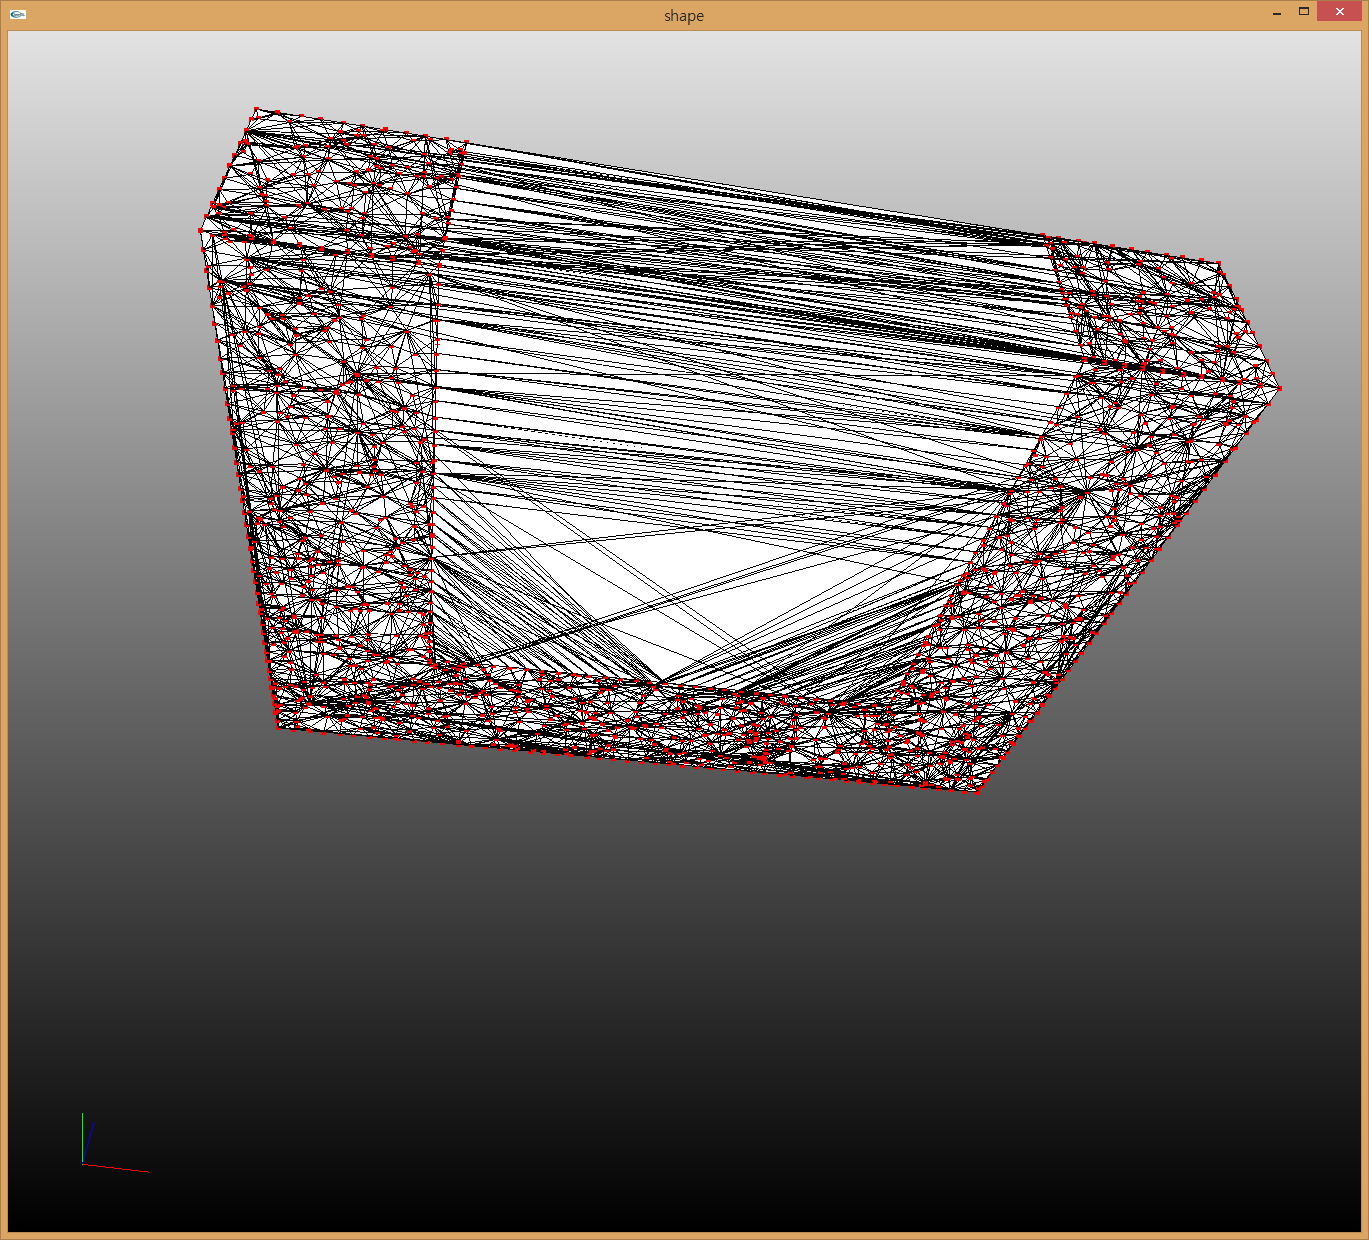
\includegraphics[width=0.22\textwidth]{img/U4.png}
     \label{fig:uOption4}
  }\hspace{-3mm}
  \caption{An 'U' example \label{fig:U}}
\end{figure*}
\begin{figure*}[hbt]
 \centering
  \subfigure[]{
    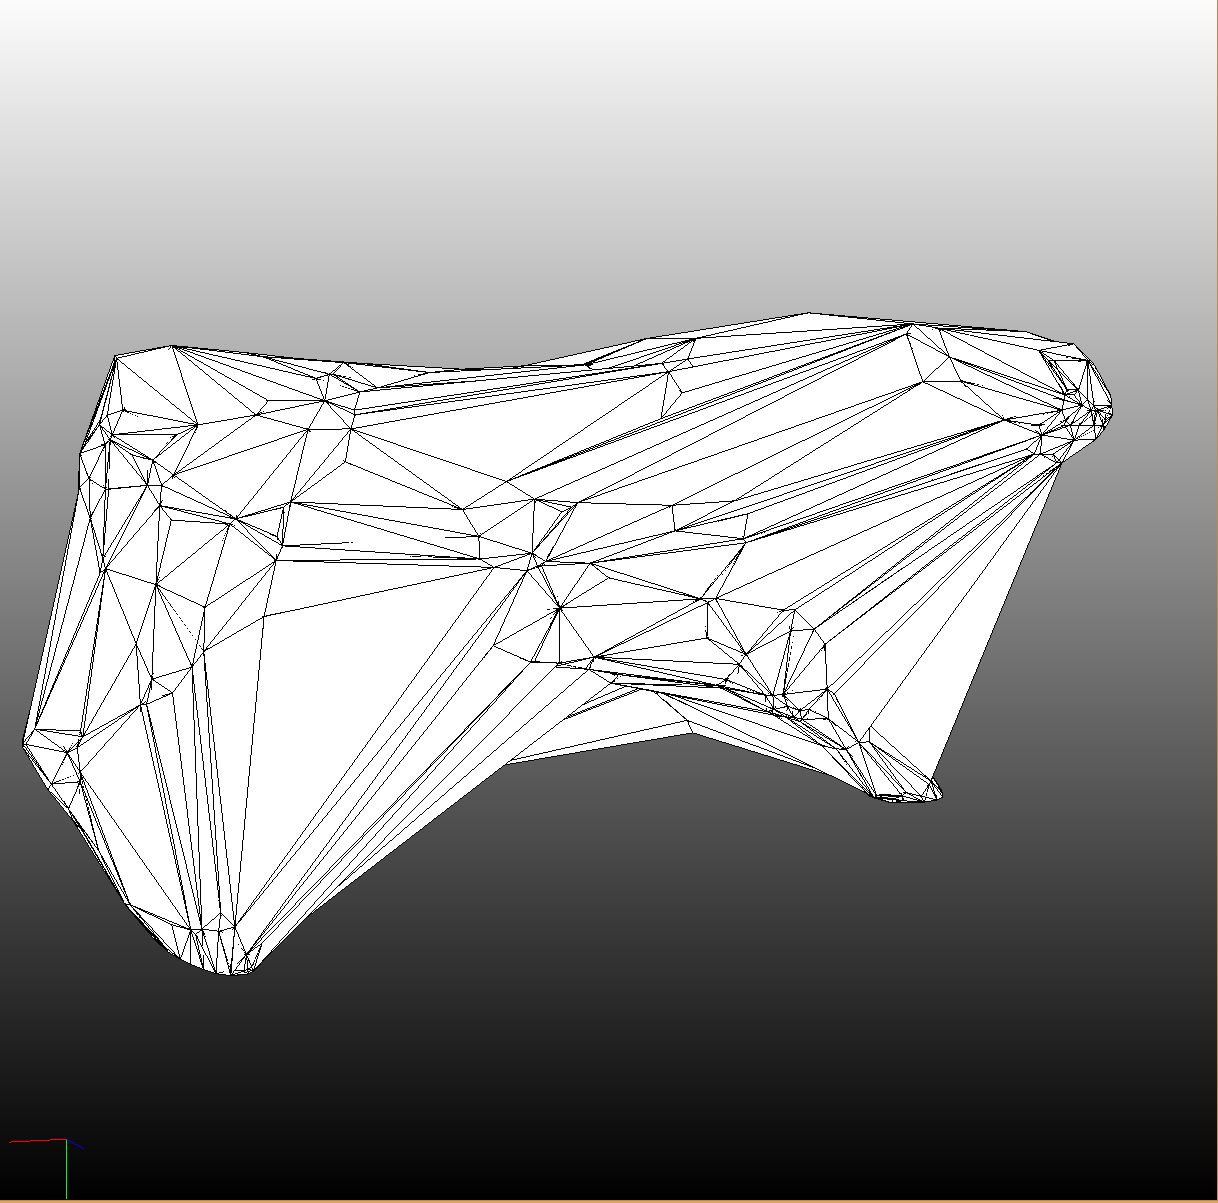
\includegraphics[width=0.22\textwidth]{img/bull3.png}
    \label{fig:bullOption3}
  }\hspace{-3mm}
  \subfigure[]{
     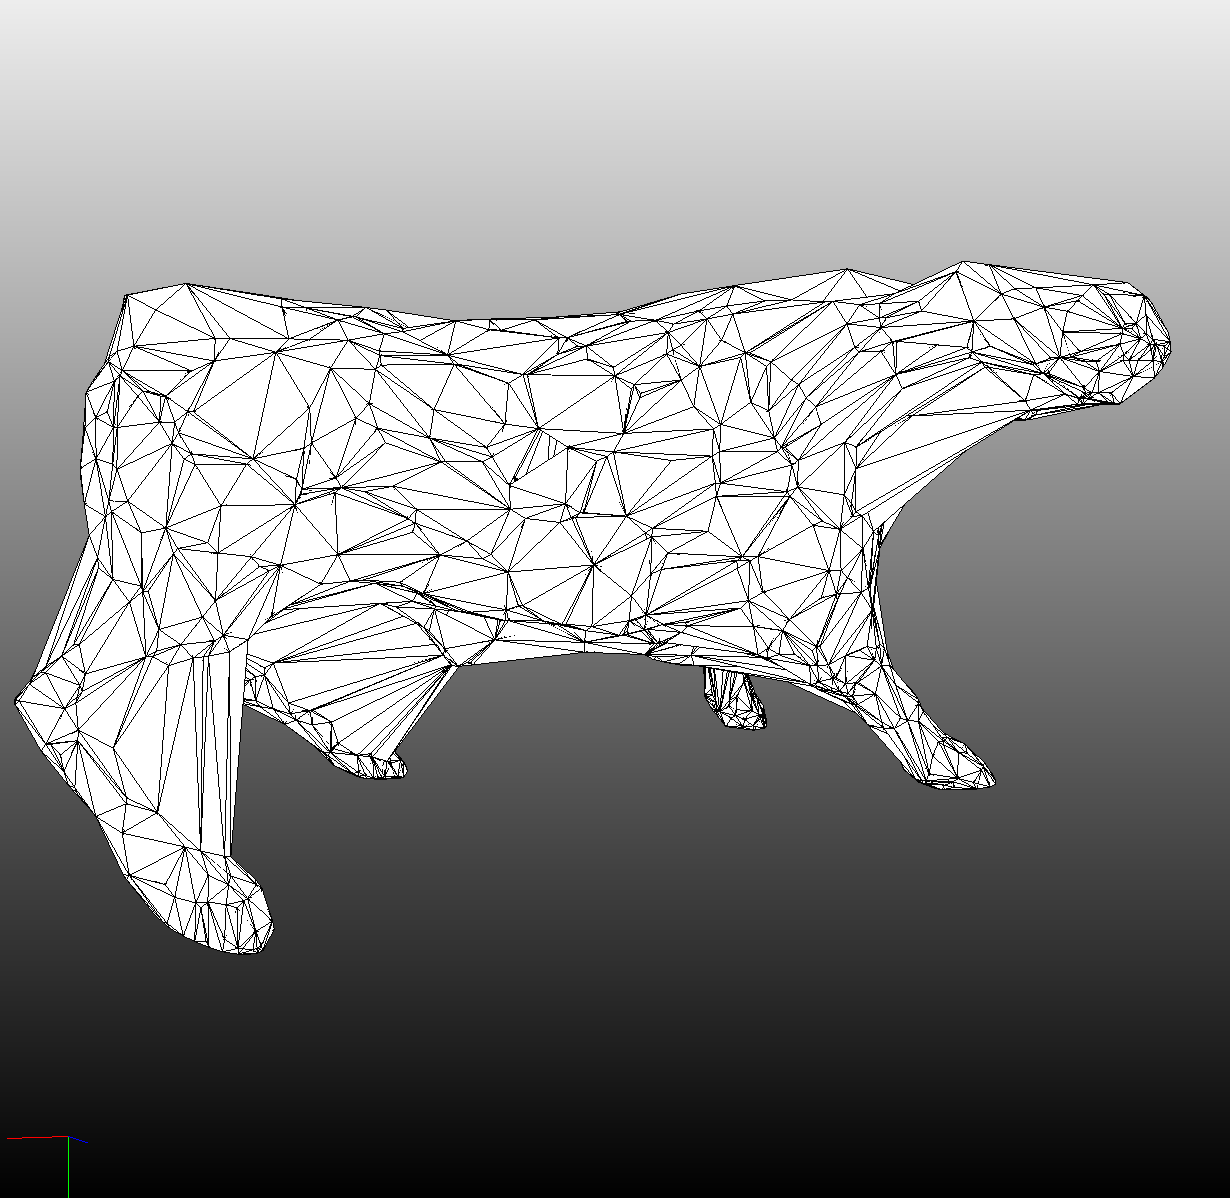
\includegraphics[width=0.22\textwidth]{img/bull2.png}
     \label{fig:bullOption2}
  }\hspace{-3mm}
  \subfigure[]{
    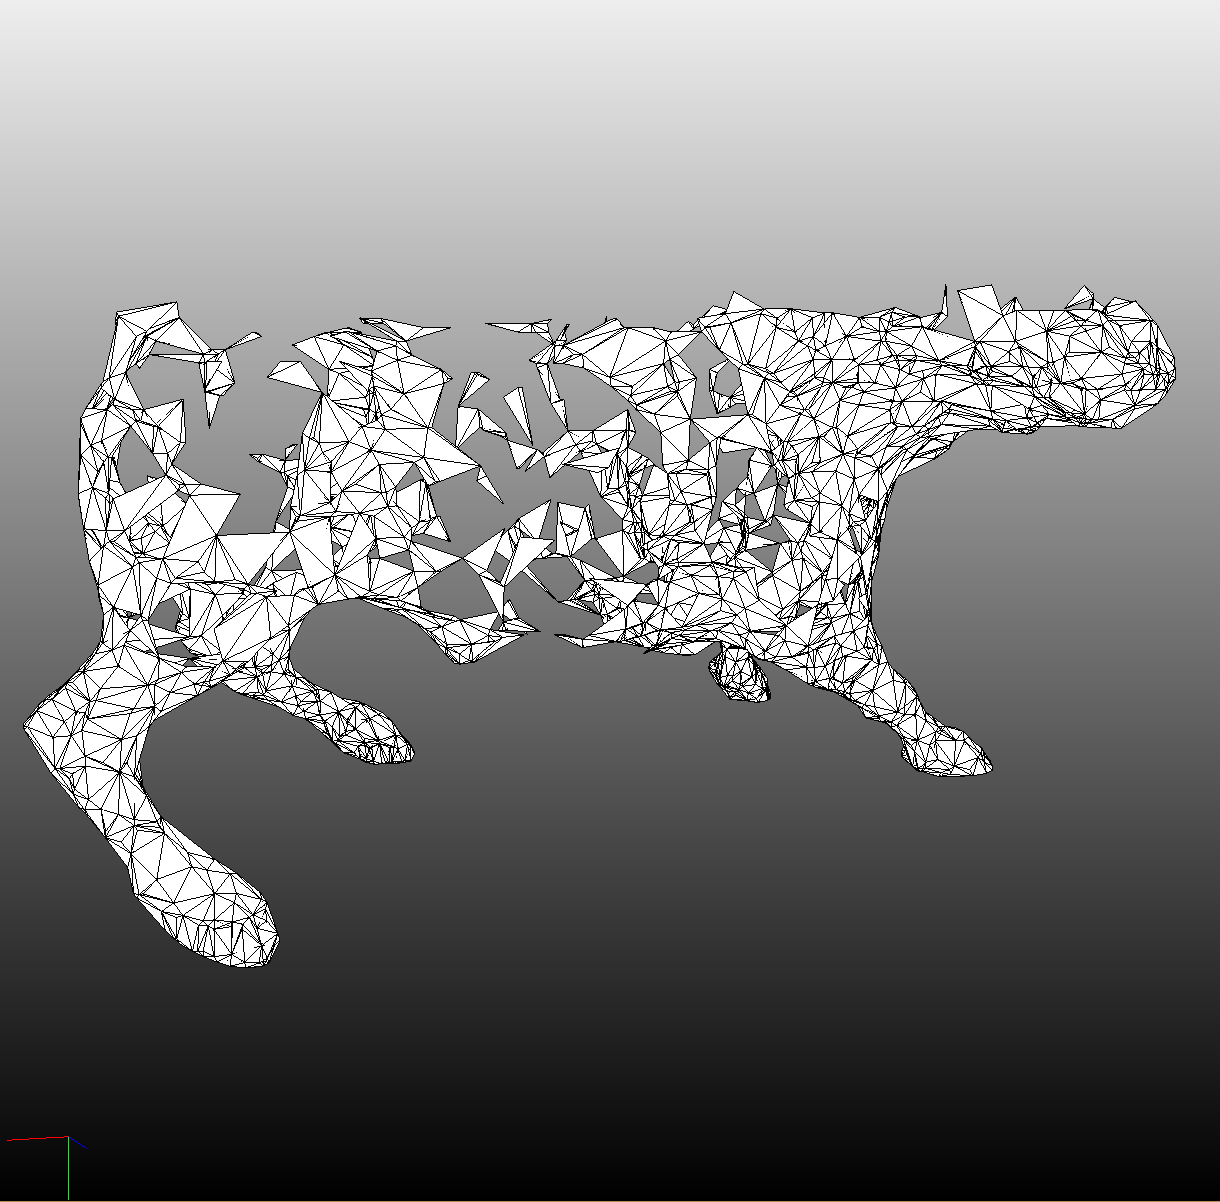
\includegraphics[width=0.22\textwidth]{img/bull1.png}
     \label{fig:bullOption1}
  }\hspace{-3mm}
  \subfigure[]{
    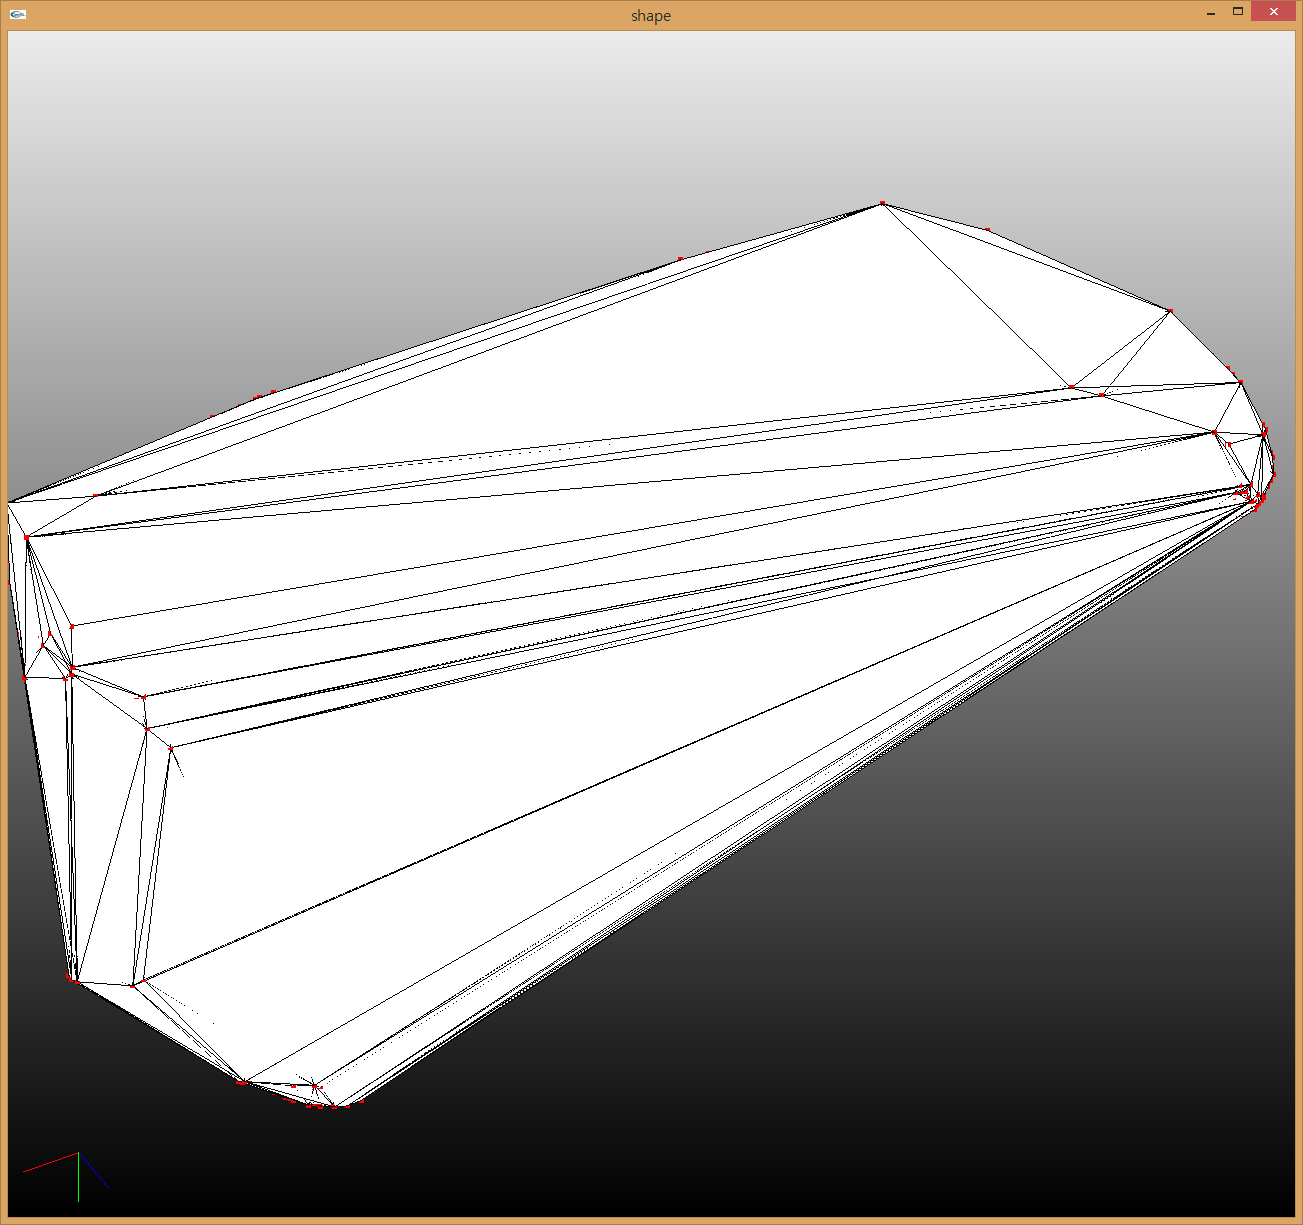
\includegraphics[width=0.22\textwidth]{img/bull4.png}
     \label{fig:bullOption4}
  }\hspace{-3mm}
  \caption{A bull example \label{fig:bull}}
\end{figure*}
\begin{figure*}[hbt]
 \centering
  \subfigure[]{
    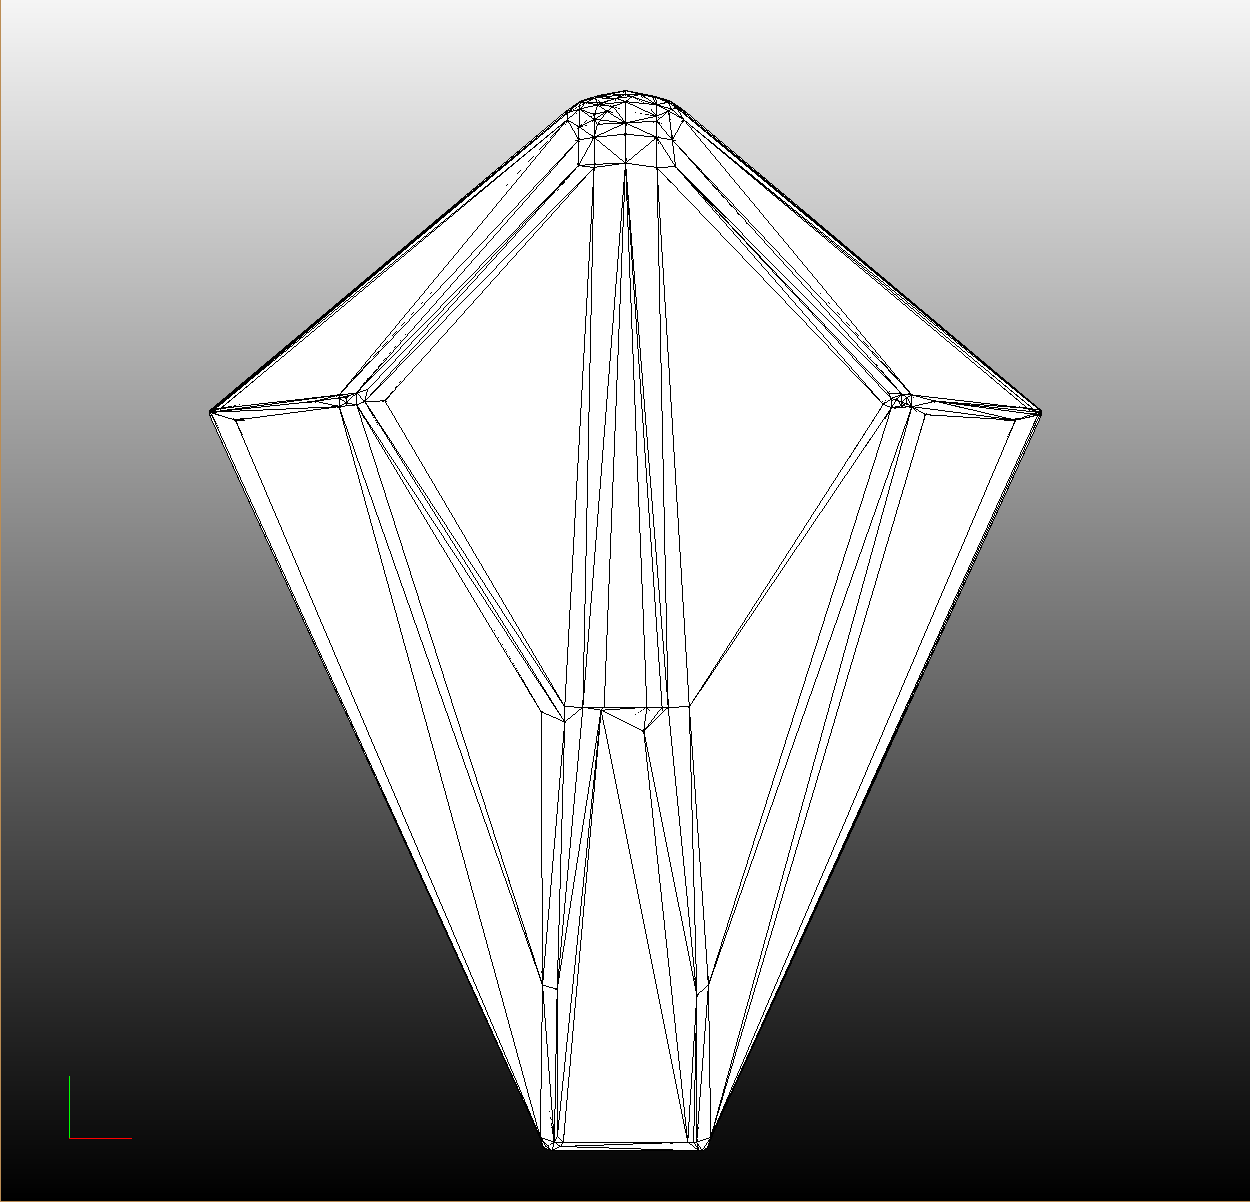
\includegraphics[width=0.22\textwidth]{img/bb3.png}
    \label{fig:bbOption3}
  }\hspace{-3mm}
  \subfigure[]{
     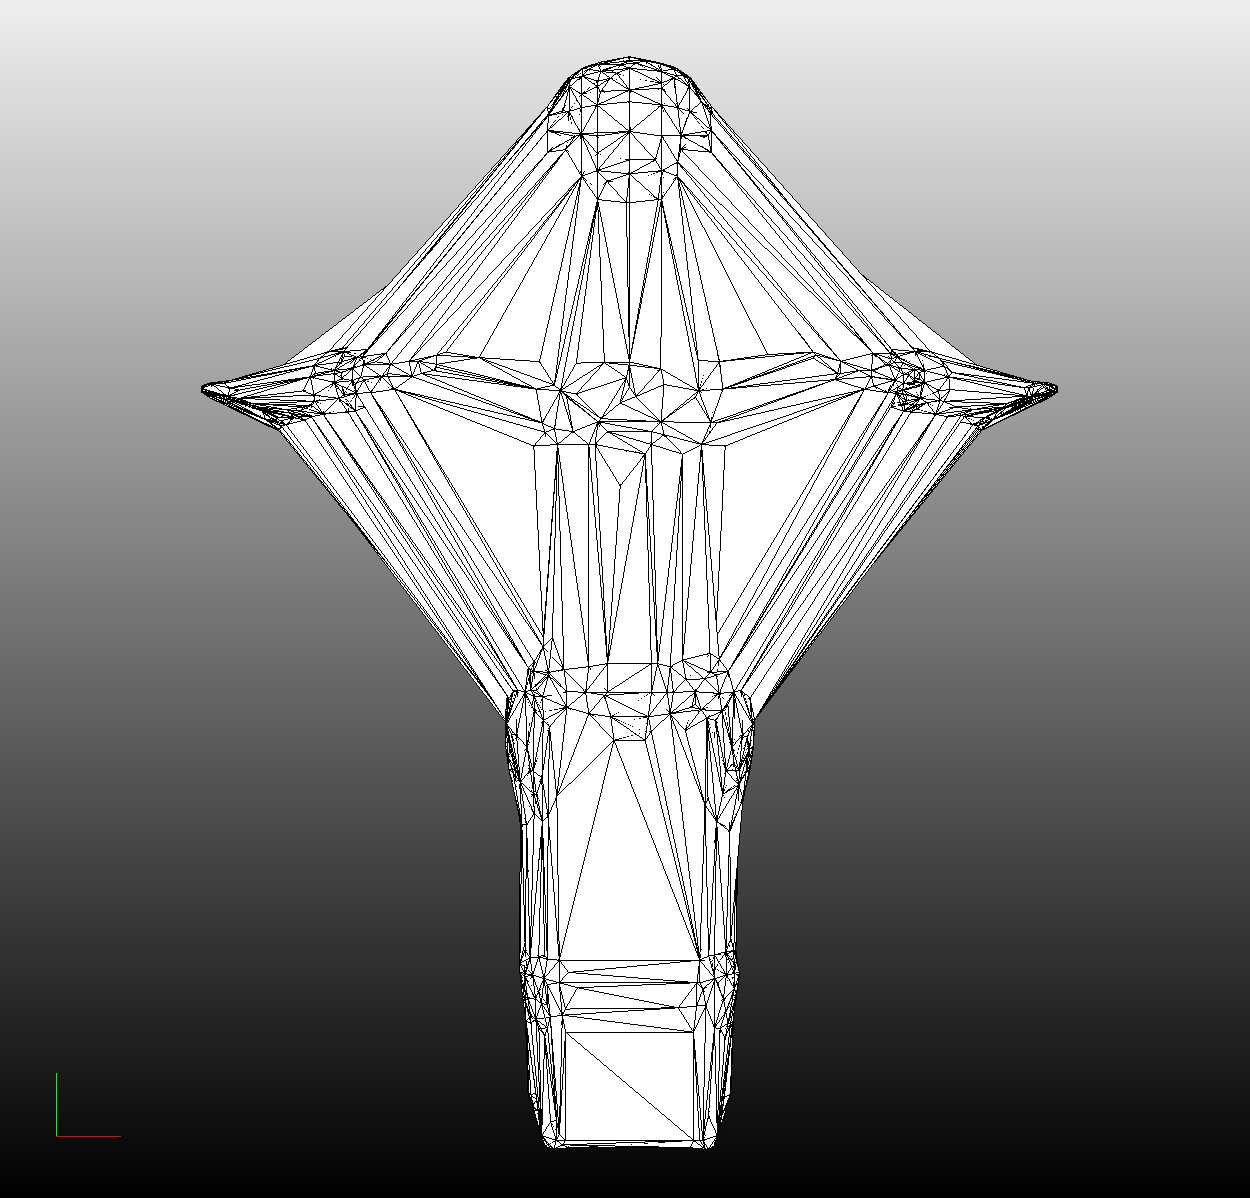
\includegraphics[width=0.22\textwidth]{img/bb2.png}
     \label{fig:bbOption2}
  }\hspace{-3mm}
  \subfigure[]{
    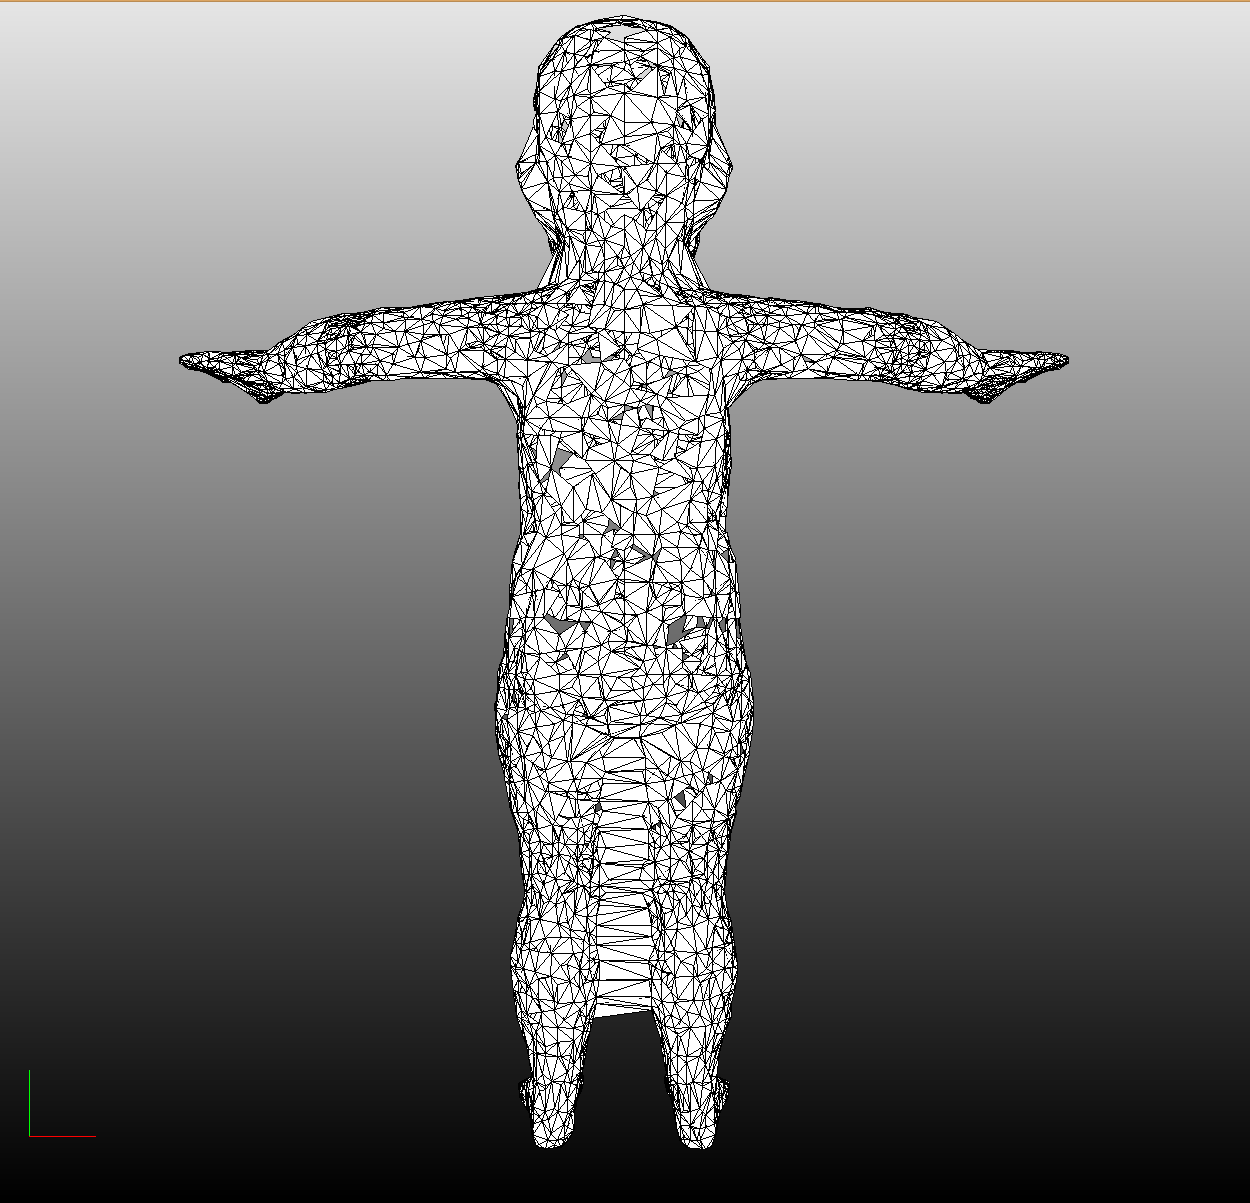
\includegraphics[width=0.22\textwidth]{img/bb1.png}
     \label{fig:bbOption1}
  }\hspace{-3mm}
  \subfigure[]{
    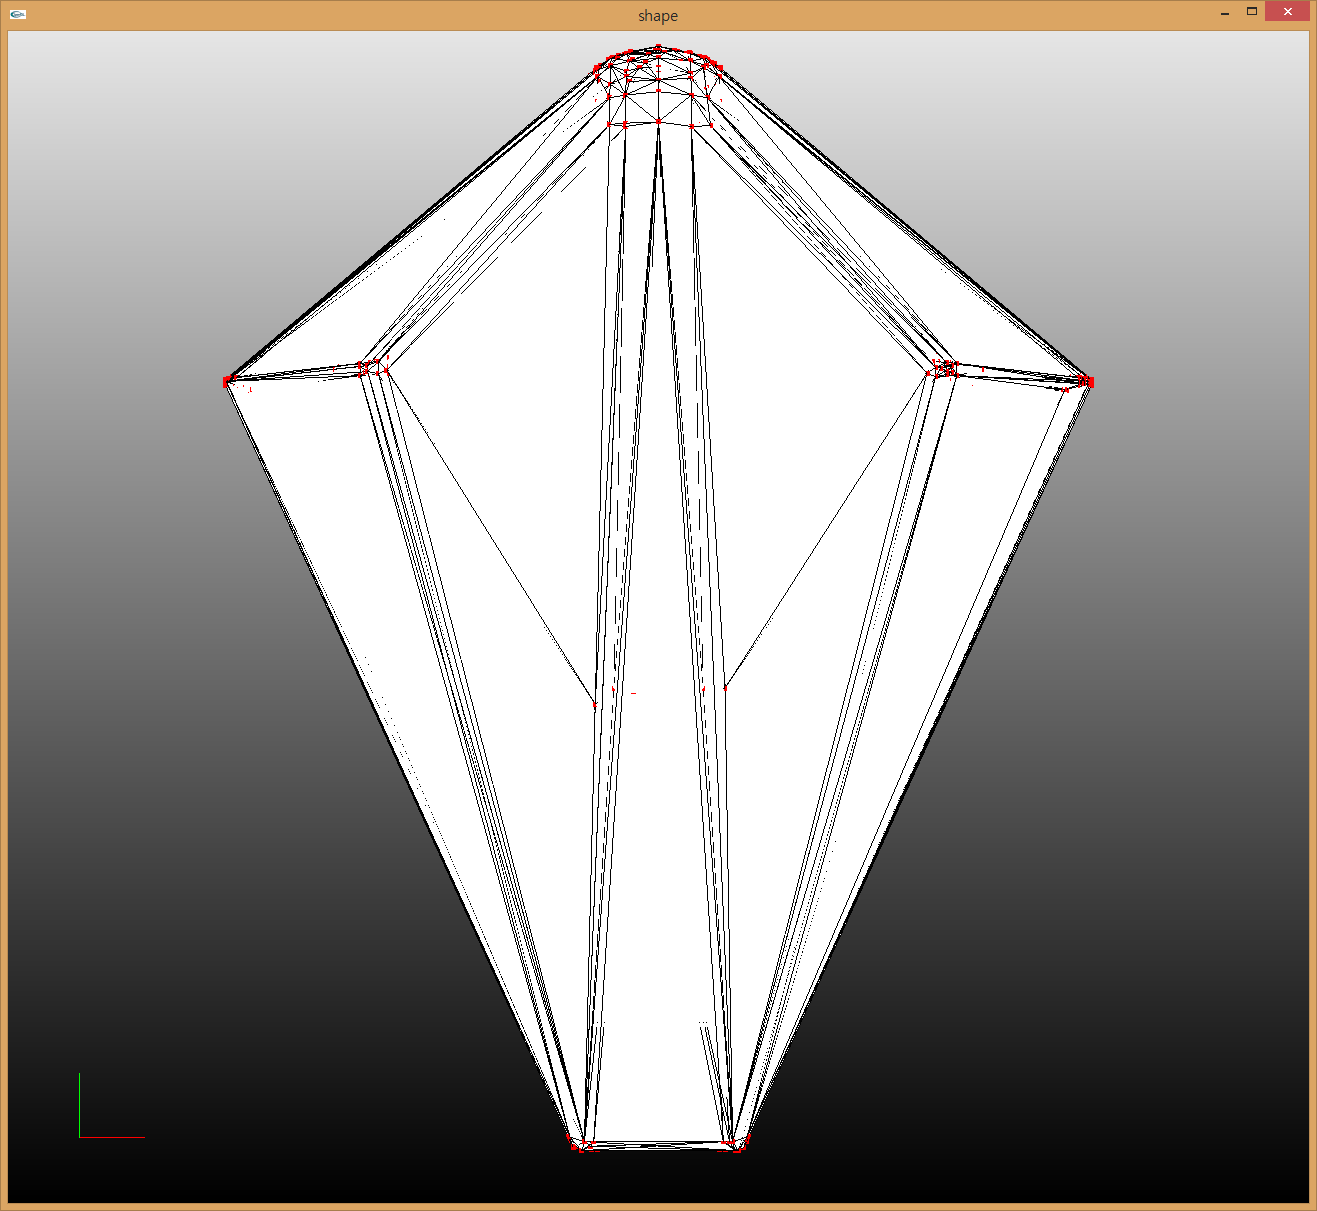
\includegraphics[width=0.22\textwidth]{img/bb4.png}
     \label{fig:bbOption4}
  }\hspace{-3mm}
  \caption{An baby example \label{fig:baby}}
\end{figure*}
\begin{figure*}[hbt]
 \centering
  \subfigure[]{
    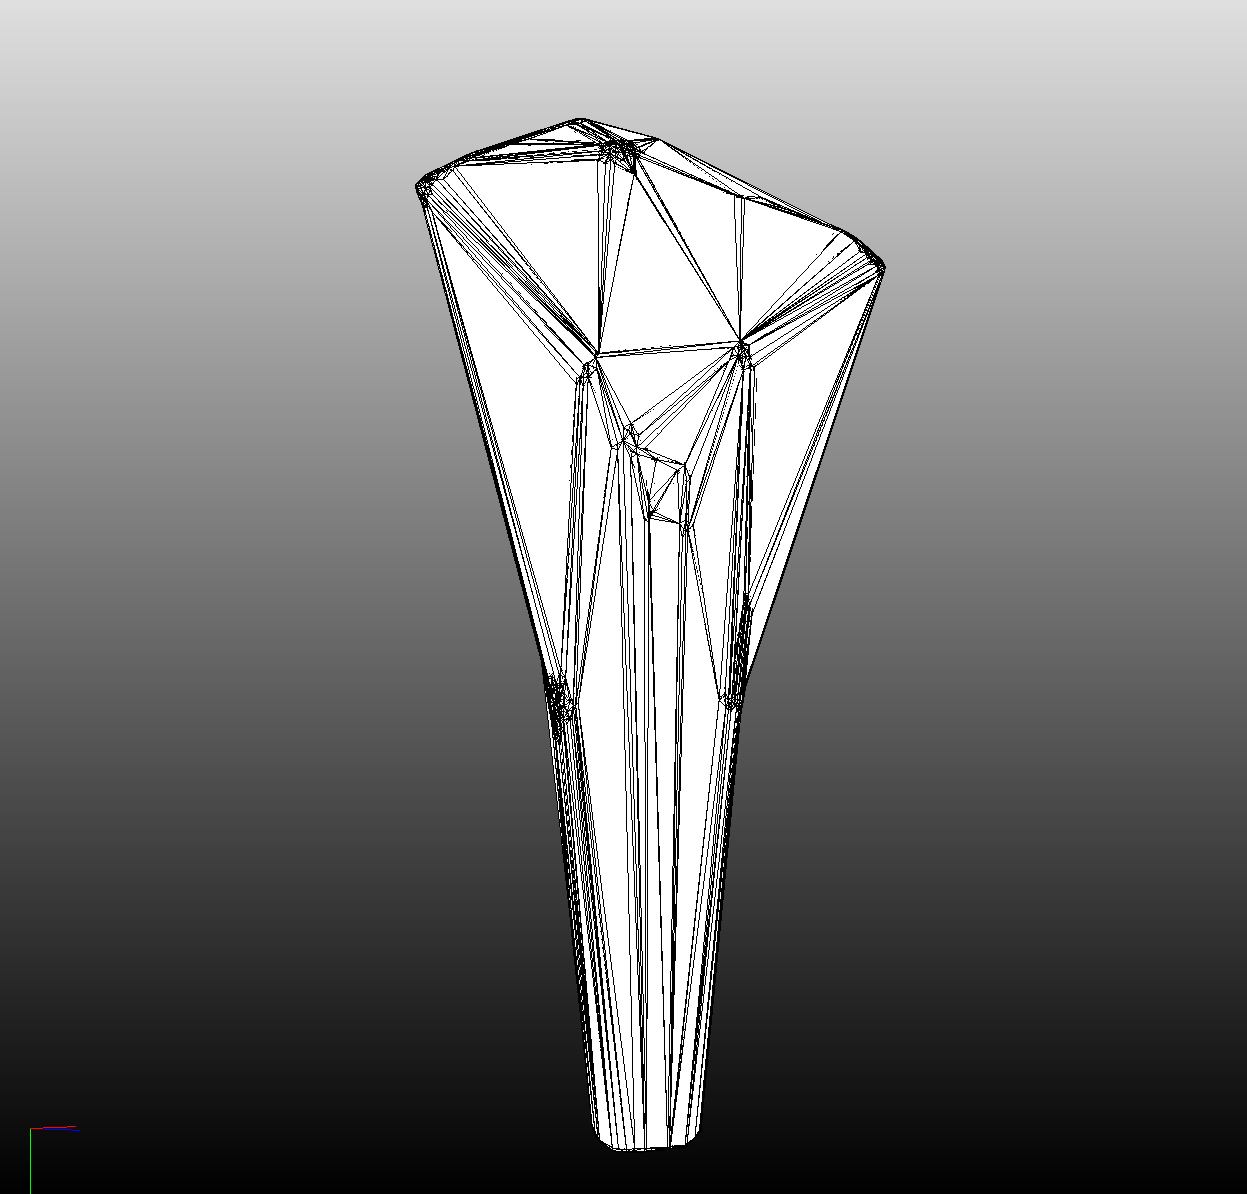
\includegraphics[width=0.22\textwidth]{img/woman3.png}
    \label{fig:womanOption3}
  }\hspace{-3mm}
  \subfigure[]{
     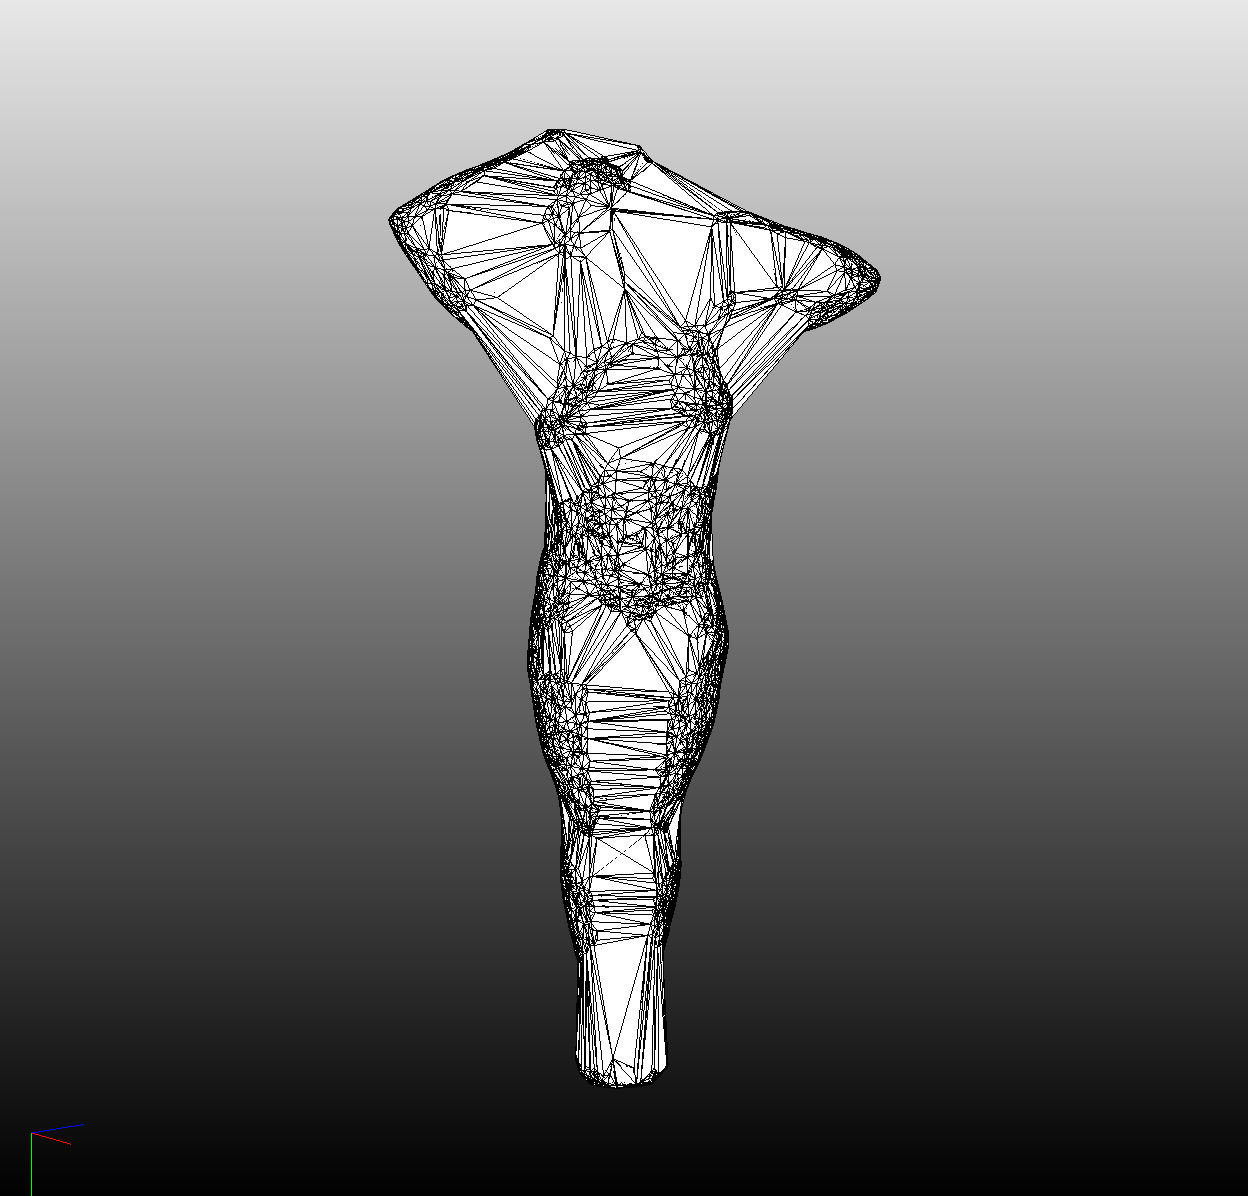
\includegraphics[width=0.22\textwidth]{img/woman2.png}
     \label{fig:womanOption2}
  }\hspace{-3mm}
  \subfigure[]{
    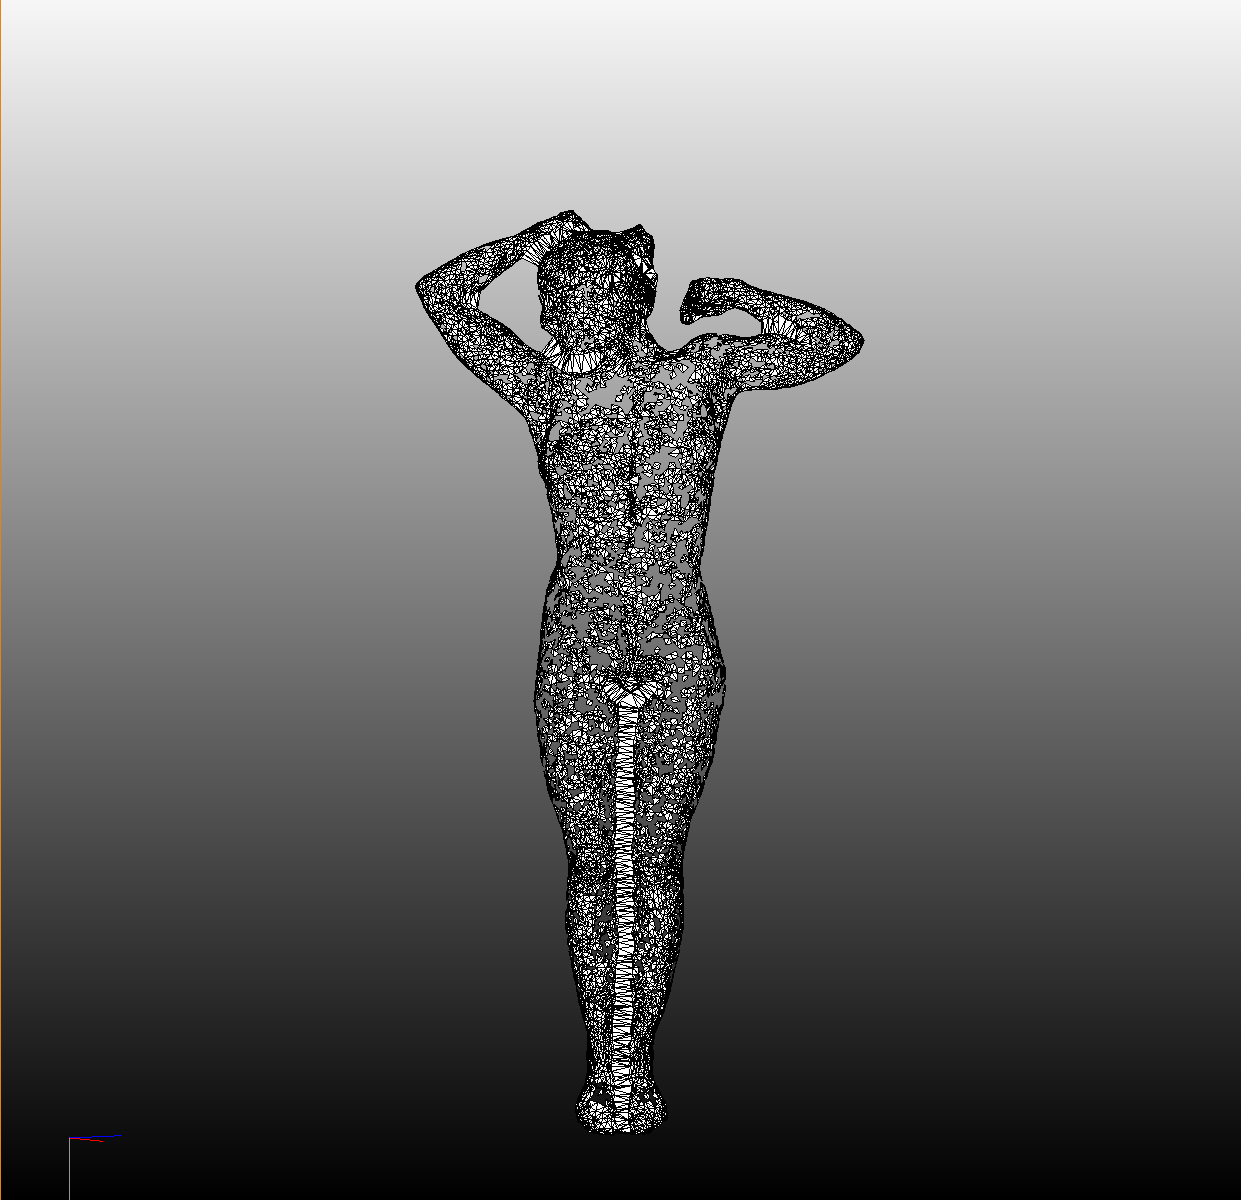
\includegraphics[width=0.22\textwidth]{img/woman1.png}
     \label{fig:womanOption1}
  }\hspace{-3mm}
  \subfigure[]{
    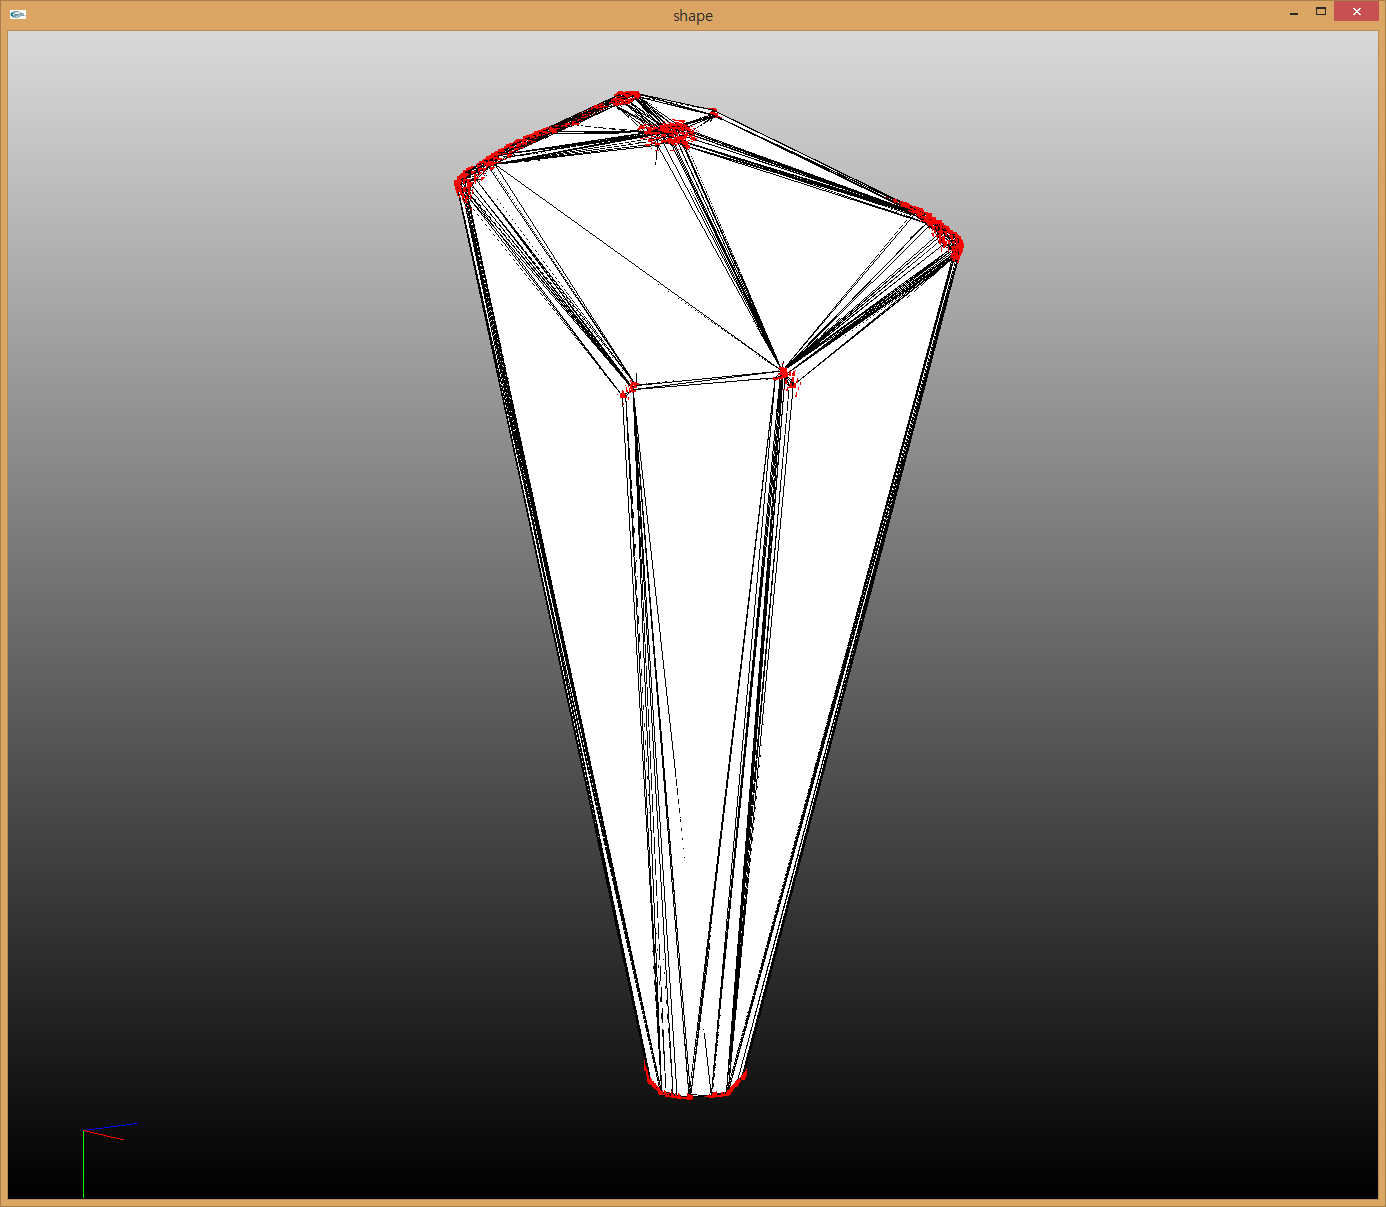
\includegraphics[width=0.22\textwidth]{img/woman4.png}
     \label{fig:womanOption4}
  }\hspace{-3mm}
  \caption{An woman example \label{fig:woman}}
\end{figure*}
\begin{figure*}[hbt]
 \centering
  \subfigure[]{
    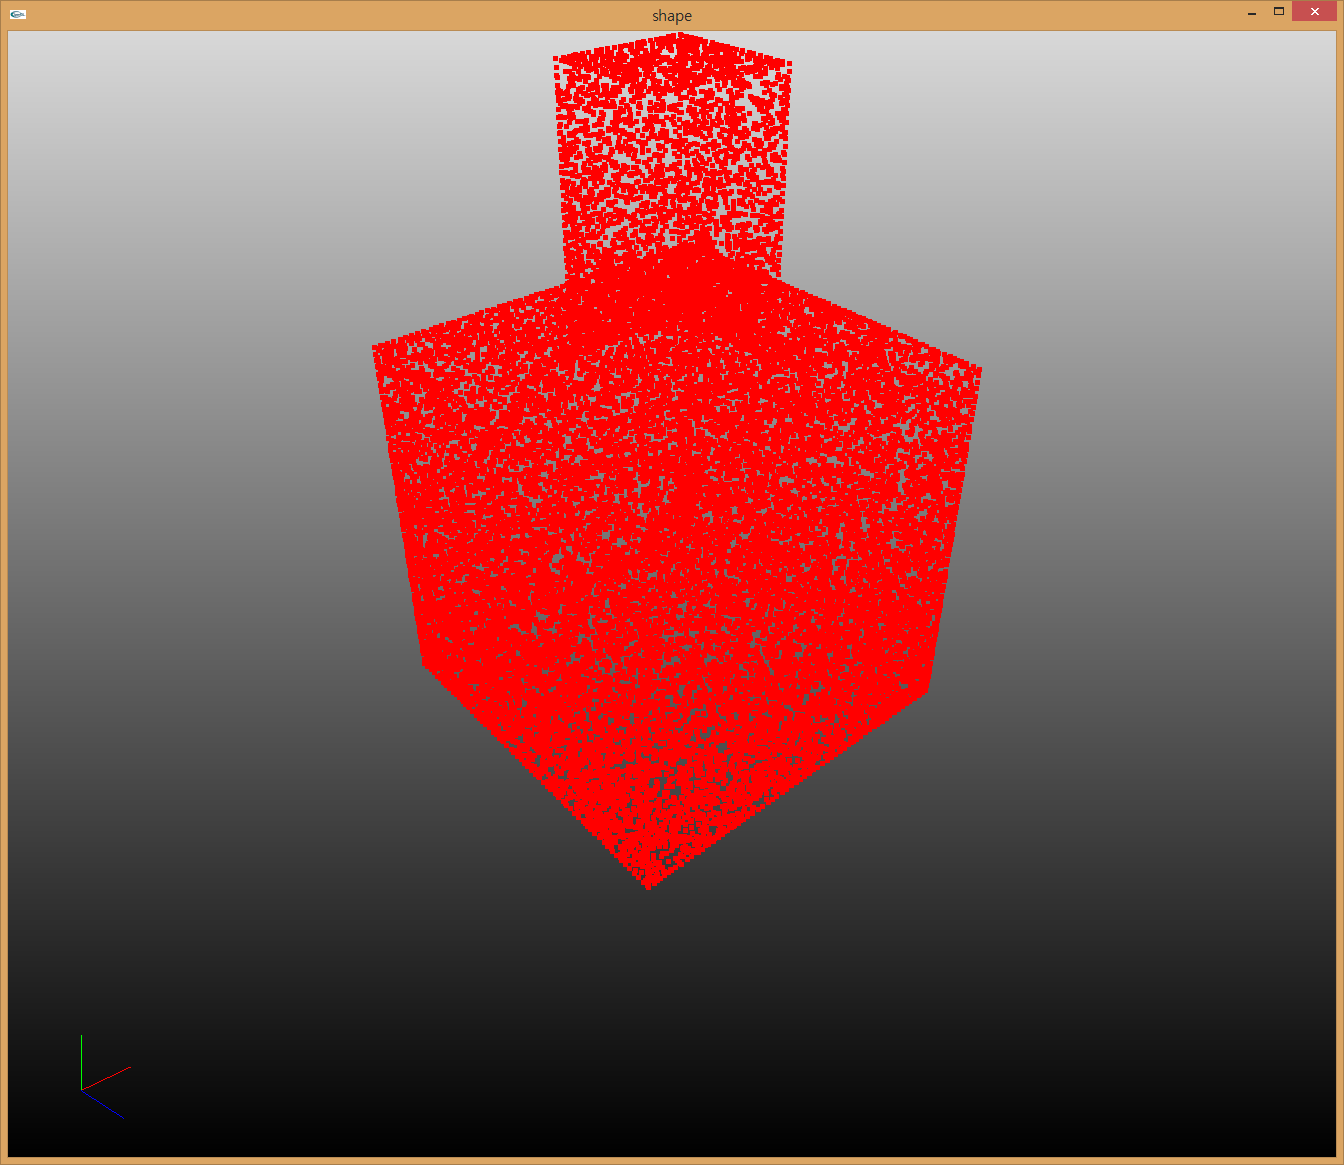
\includegraphics[width=0.22\textwidth]{img/TT3.png}
    \label{fig:ttOption3}
  }\hspace{-3mm}
  \subfigure[]{
     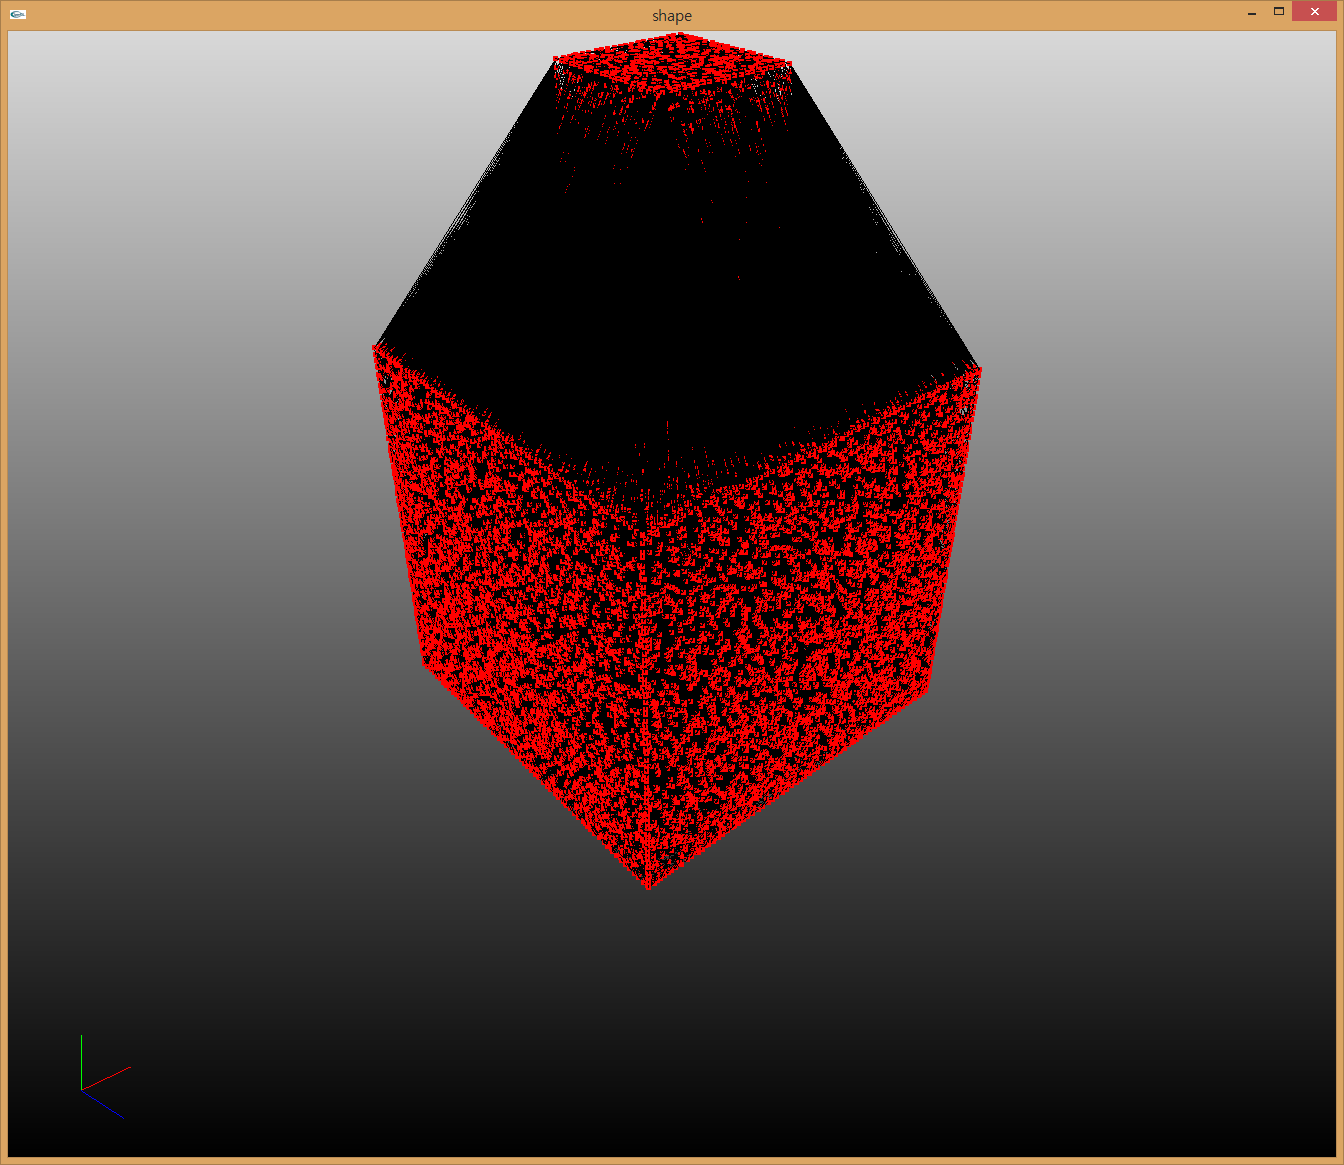
\includegraphics[width=0.22\textwidth]{img/TT2.png}
     \label{fig:ttOption2}
  }\hspace{-3mm}
  \subfigure[]{
    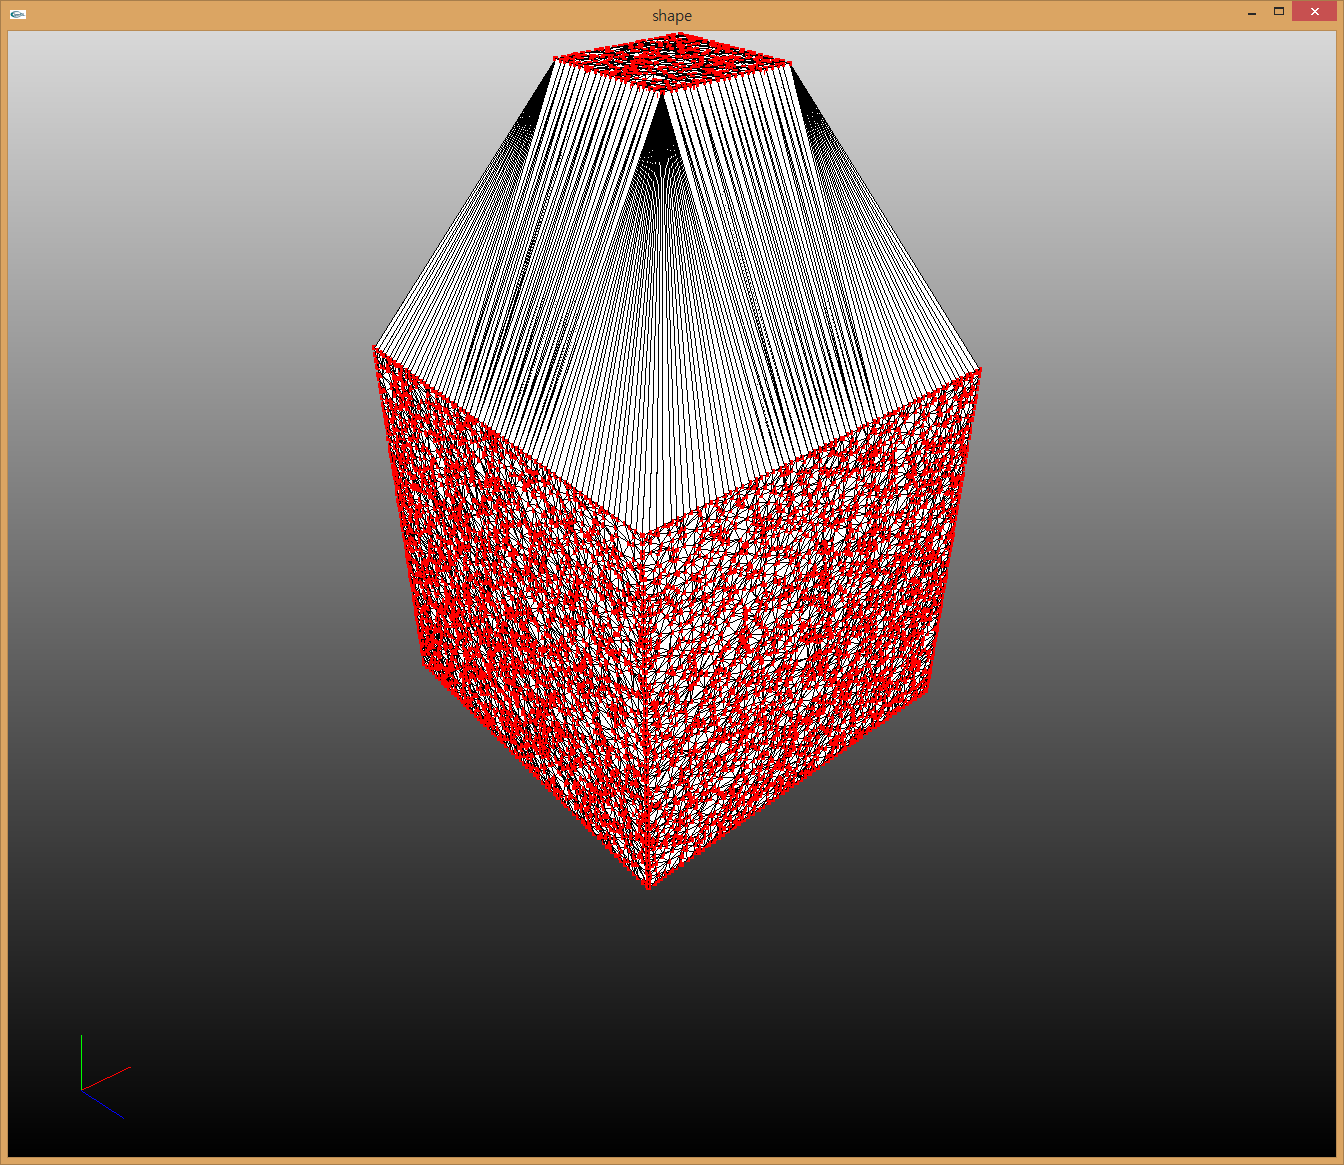
\includegraphics[width=0.22\textwidth]{img/TT1.png}
     \label{fig:ttOption1}
  }\hspace{-3mm}
  \subfigure[]{
    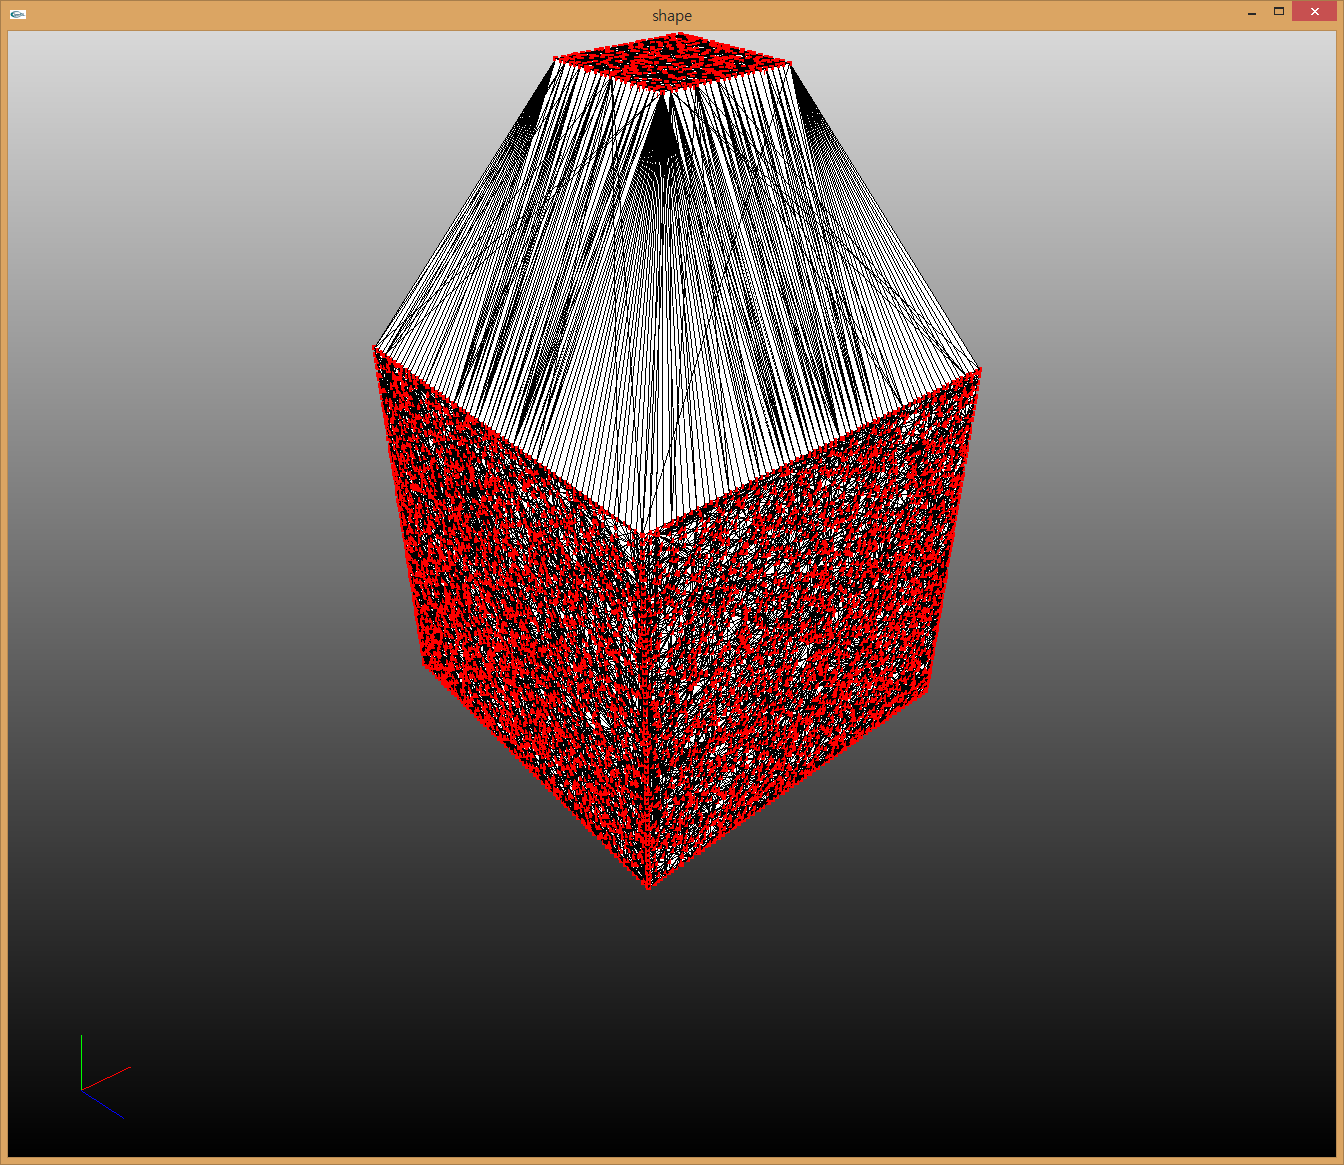
\includegraphics[width=0.22\textwidth]{img/TT4.png}
     \label{fig:ttOption4}
  }\hspace{-3mm}
  \caption{A 'T' example \label{fig:TT}}
\end{figure*}
\begin{figure*}[hbt]
 \centering
  \subfigure[]{
    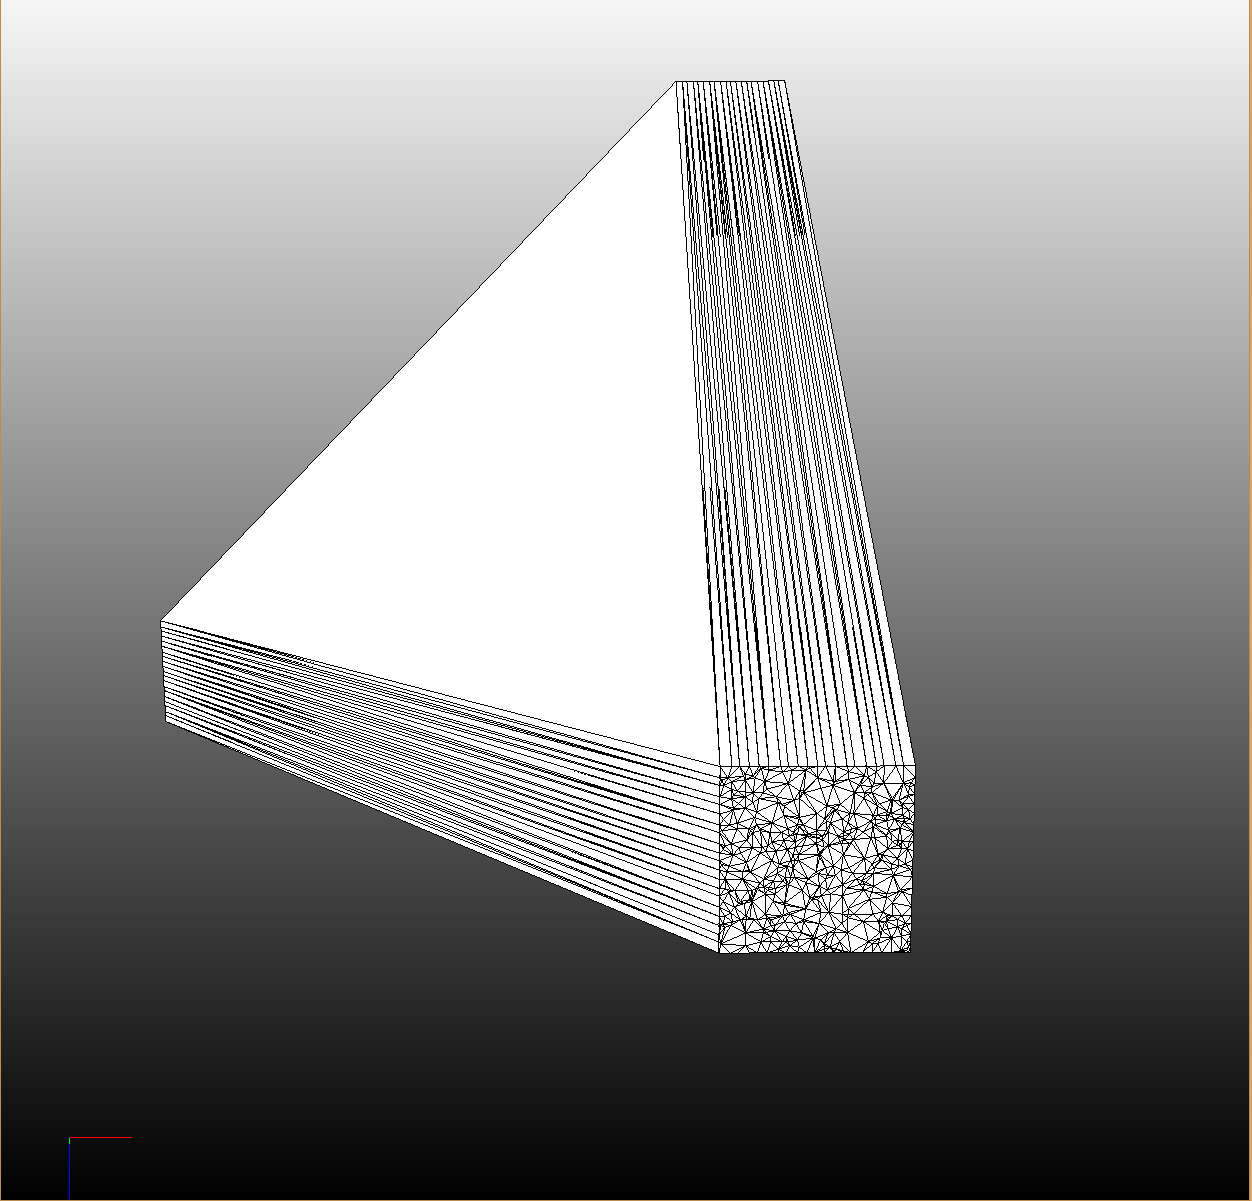
\includegraphics[width=0.22\textwidth]{img/Y3.png}
    \label{fig:yOption3}
  }\hspace{-3mm}
  \subfigure[]{
     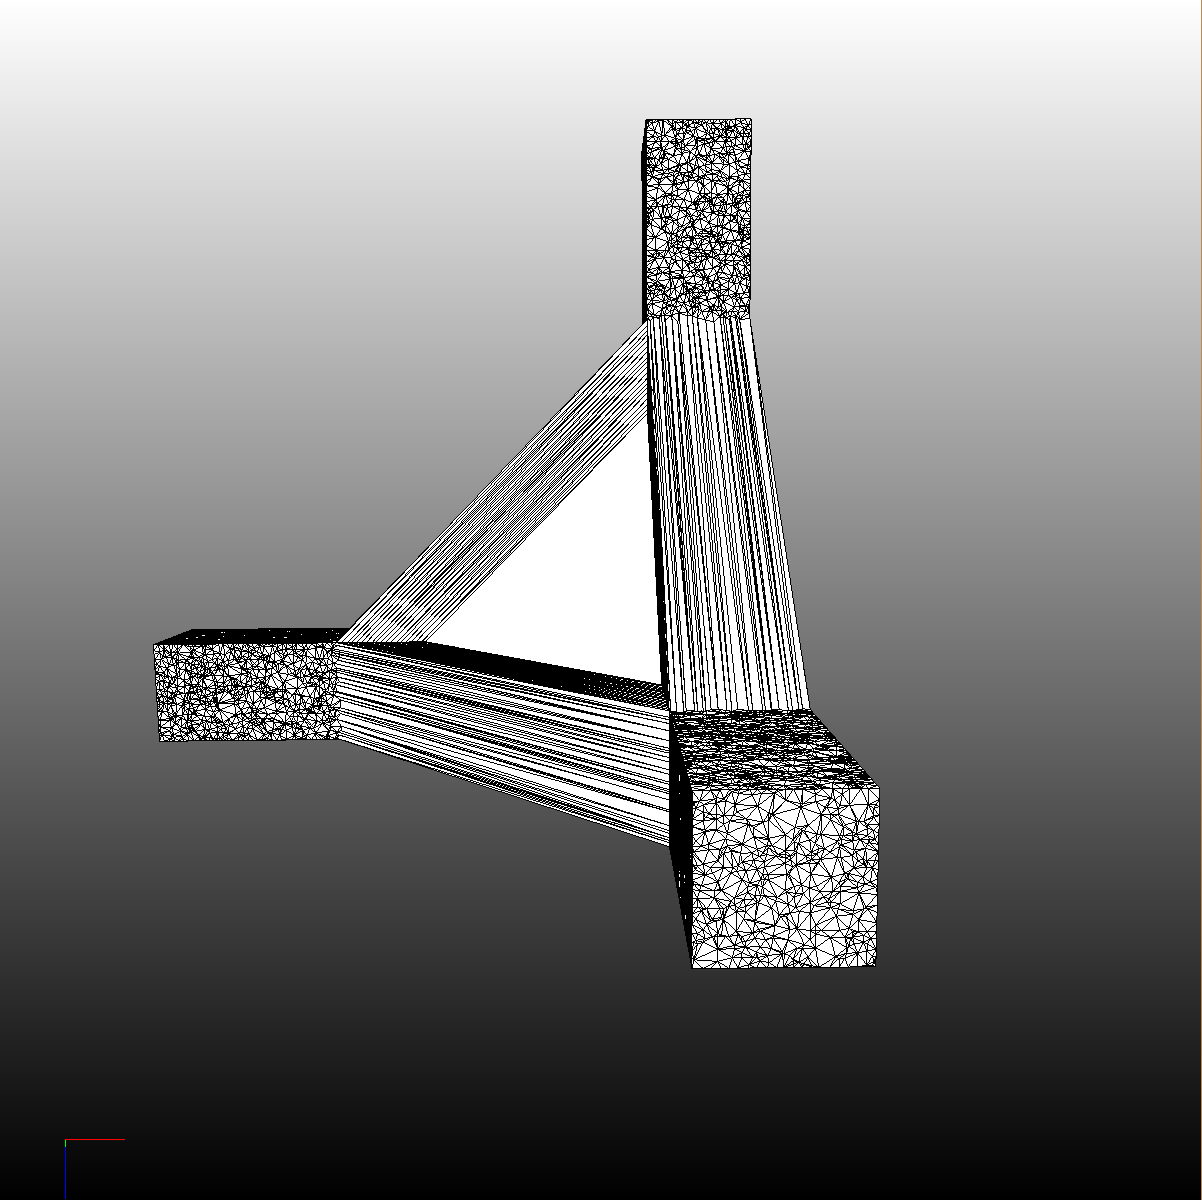
\includegraphics[width=0.22\textwidth]{img/Y2.png}
     \label{fig:yOption2}
  }\hspace{-3mm}
  \subfigure[]{
    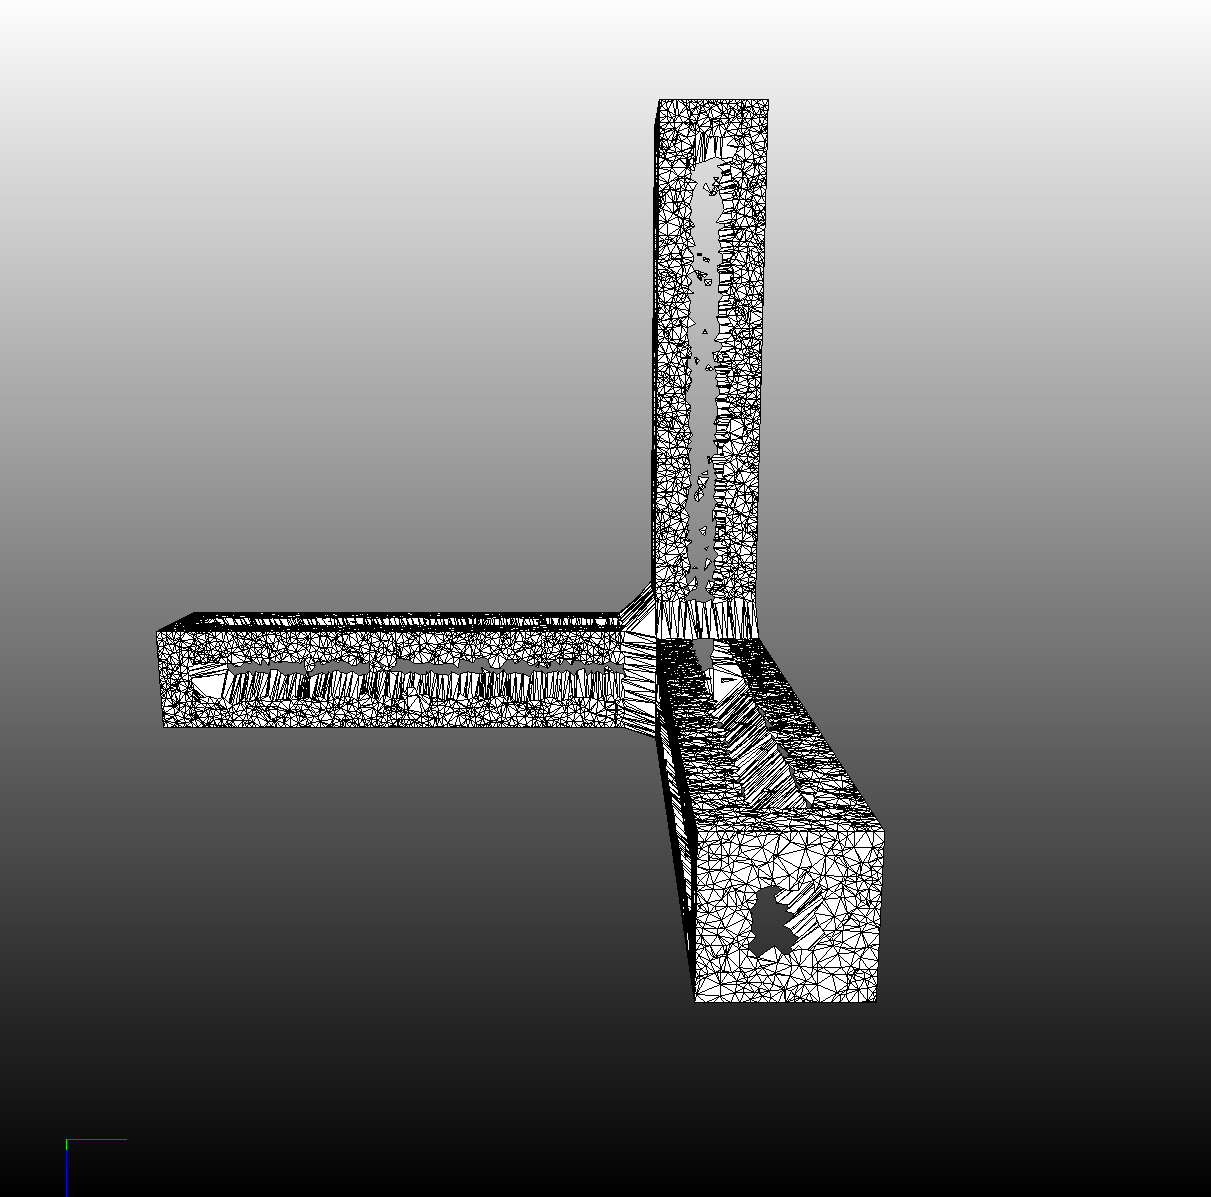
\includegraphics[width=0.22\textwidth]{img/Y1.png}
     \label{fig:yOption1}
  }\hspace{-3mm}
  \subfigure[]{
    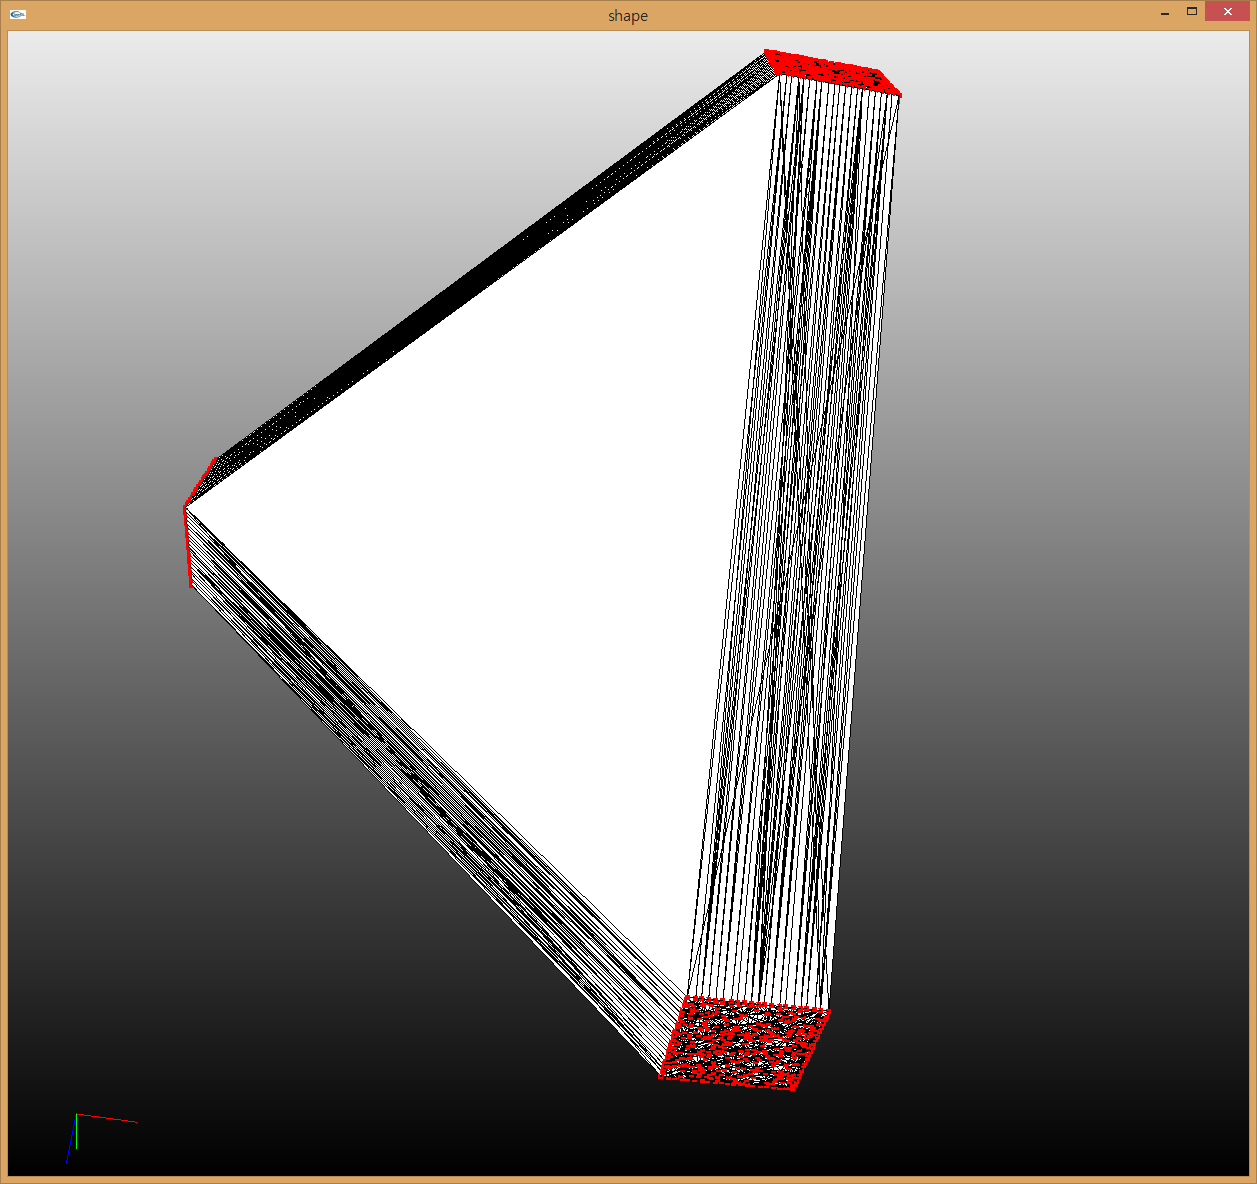
\includegraphics[width=0.22\textwidth]{img/Y4.png}
     \label{fig:yOption4}
  }\hspace{-3mm}
  \caption{An 'Y' example \label{fig:Y}}
\end{figure*}
\begin{figure*}[hbt]
 \centering
  \subfigure[]{
    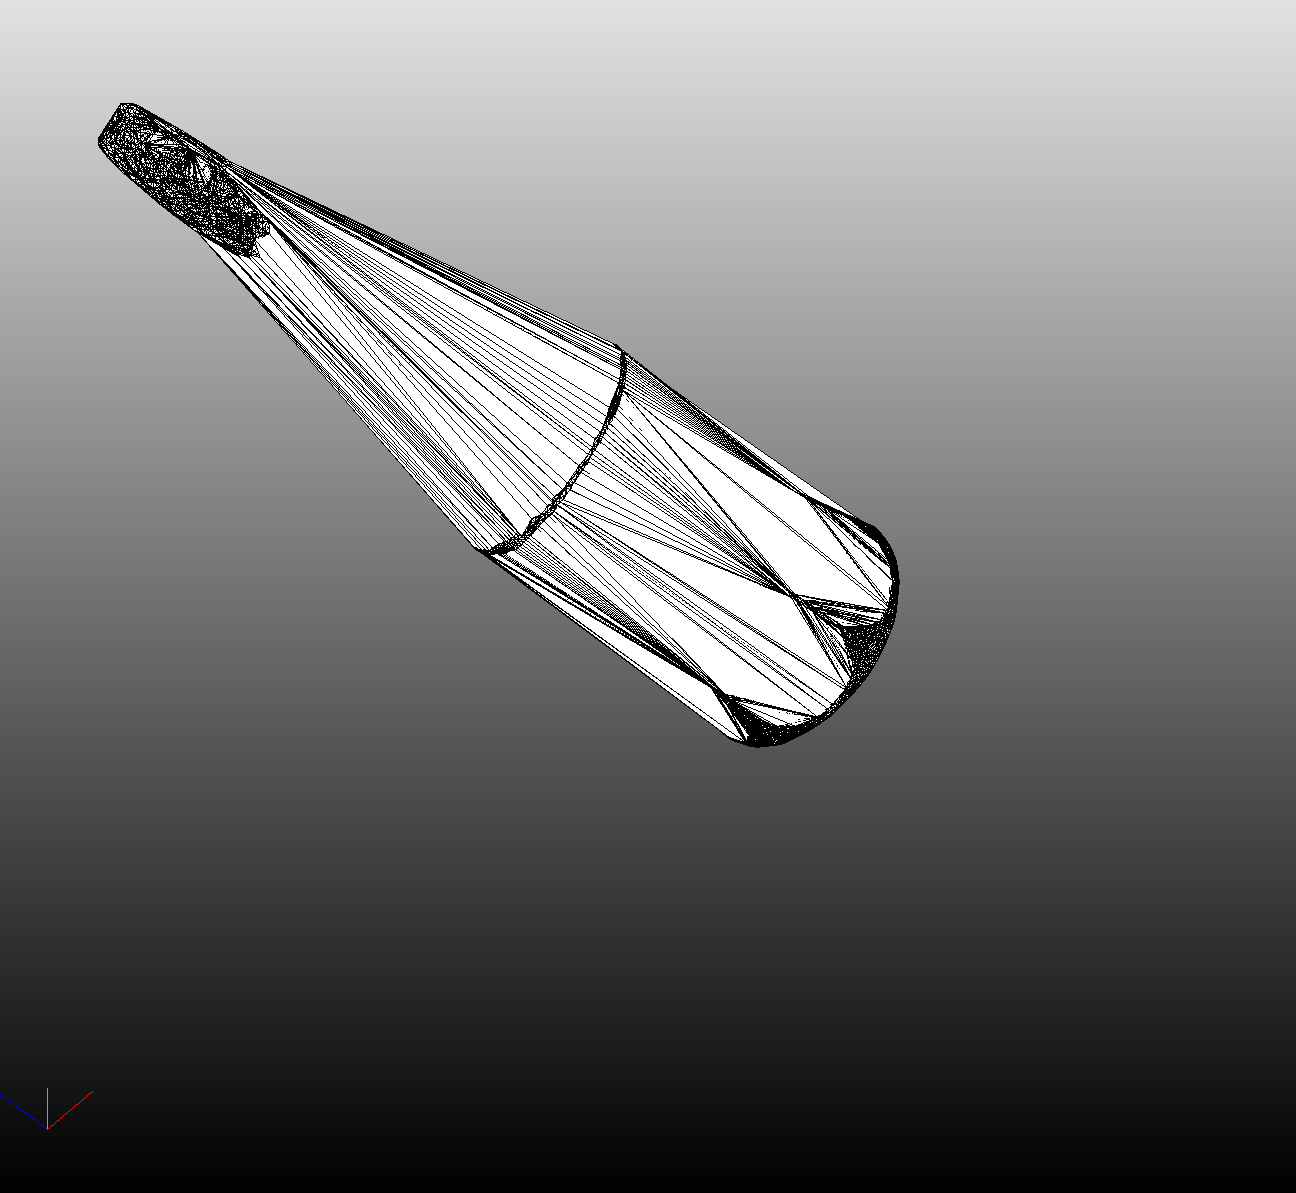
\includegraphics[width=0.22\textwidth]{img/sd3.png}
    \label{fig:sdOption3}
  }\hspace{-3mm}
  \subfigure[]{
     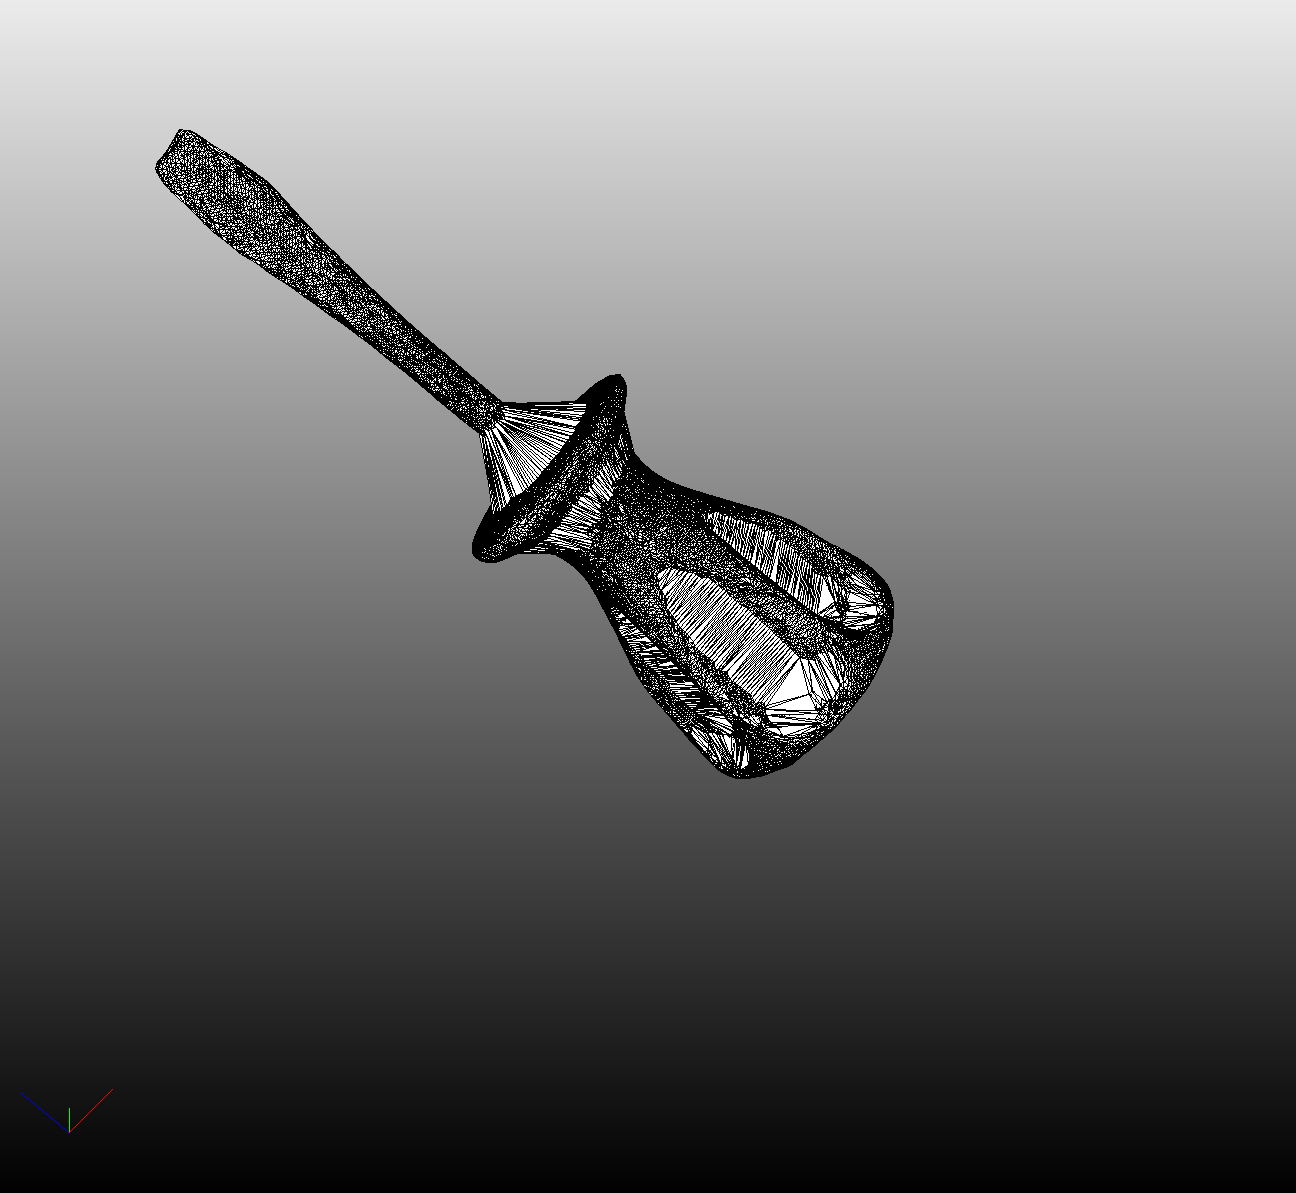
\includegraphics[width=0.22\textwidth]{img/sd2.png}
     \label{fig:sdOption2}
  }\hspace{-3mm}
  \subfigure[]{
    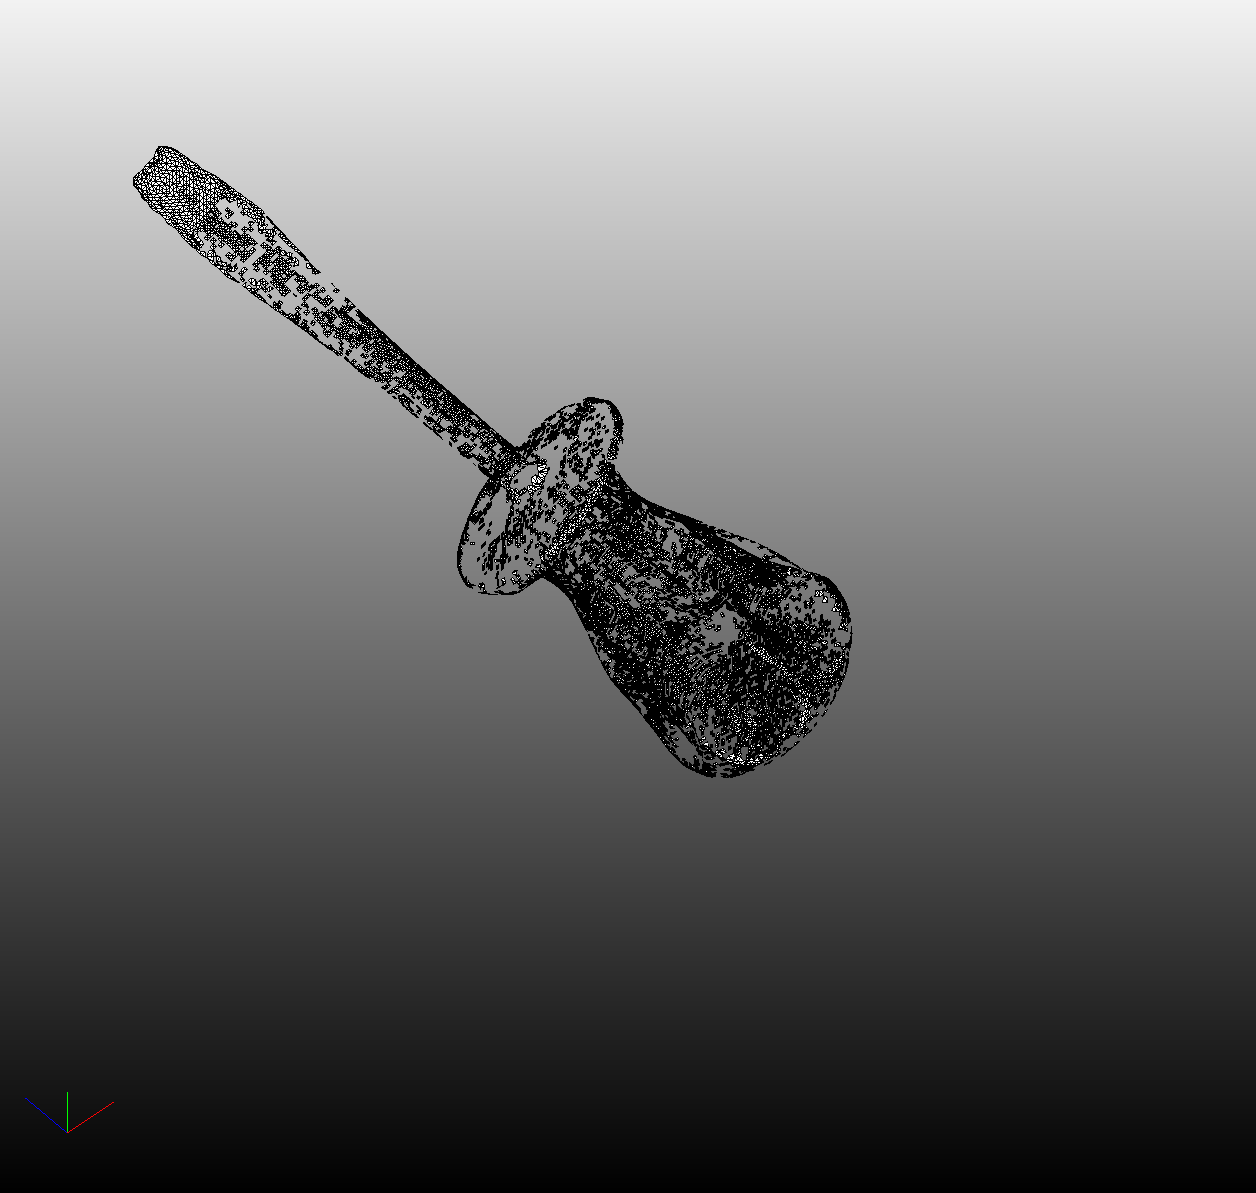
\includegraphics[width=0.22\textwidth]{img/sd1.png}
     \label{fig:sdOption1}
  }\hspace{-3mm}
  \subfigure[]{
    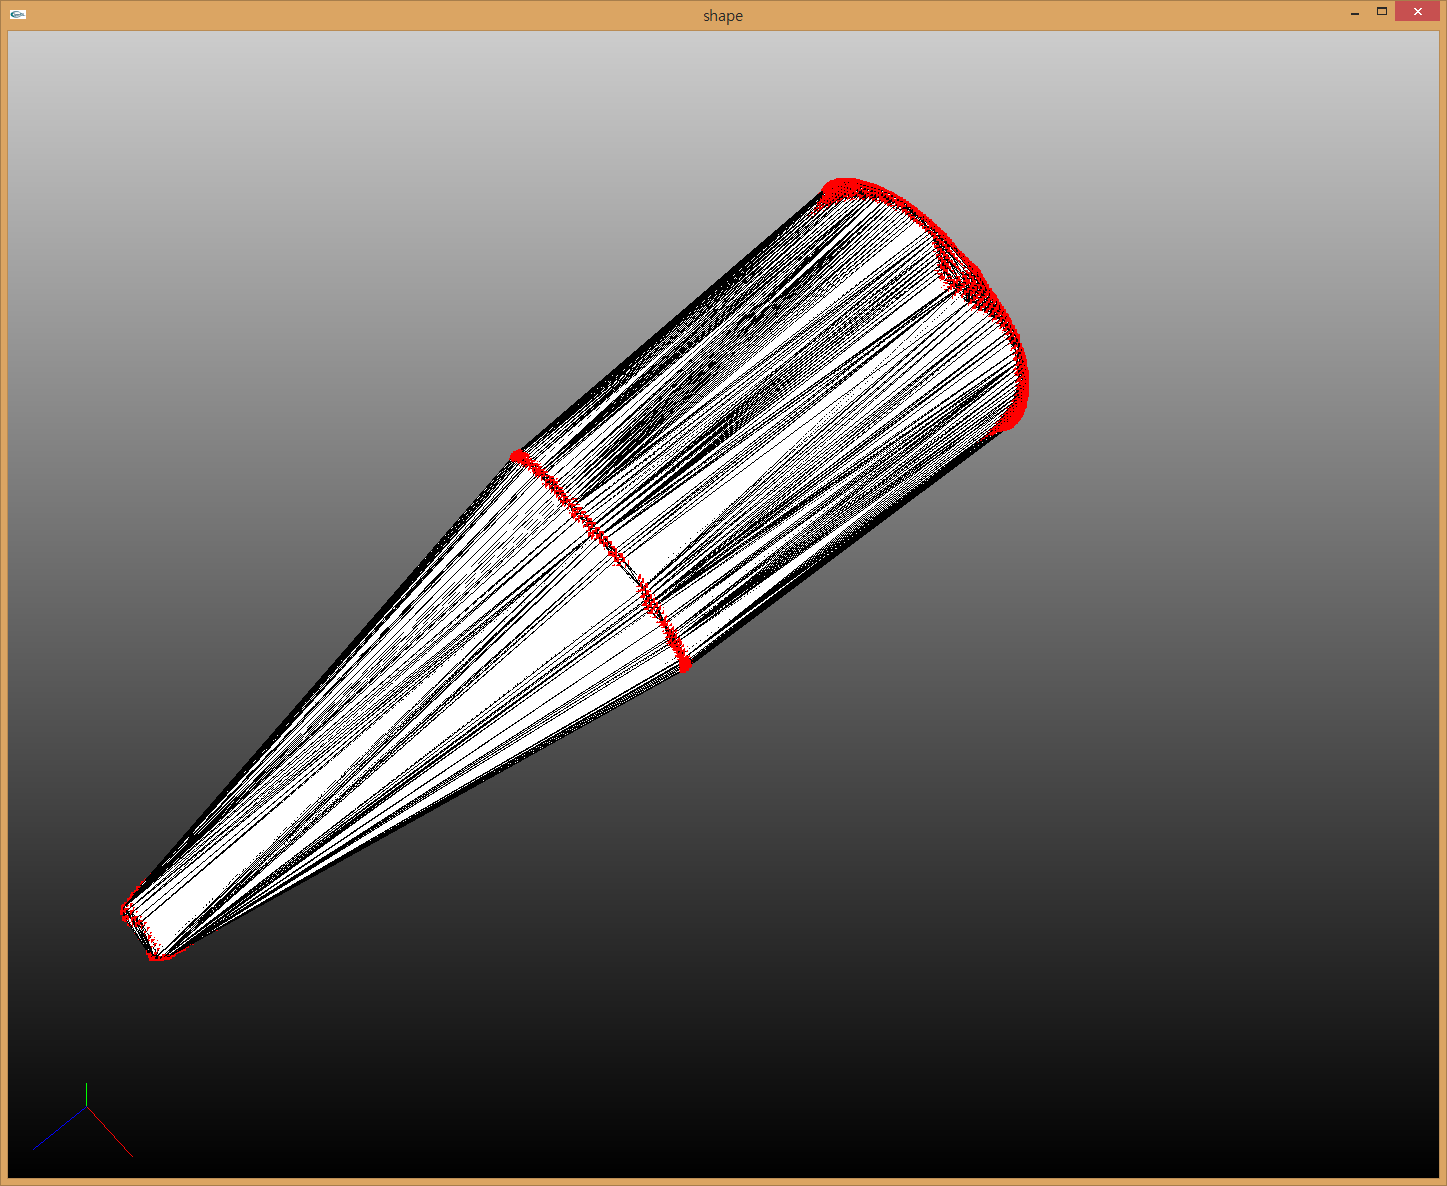
\includegraphics[width=0.22\textwidth]{img/sd4.png}
     \label{fig:sdOption4}
  }\hspace{-3mm}
  \caption{A screwdriver example \label{fig:sd}}
\end{figure*}
\begin{figure*}[hbt]
 \centering
  \subfigure[]{
    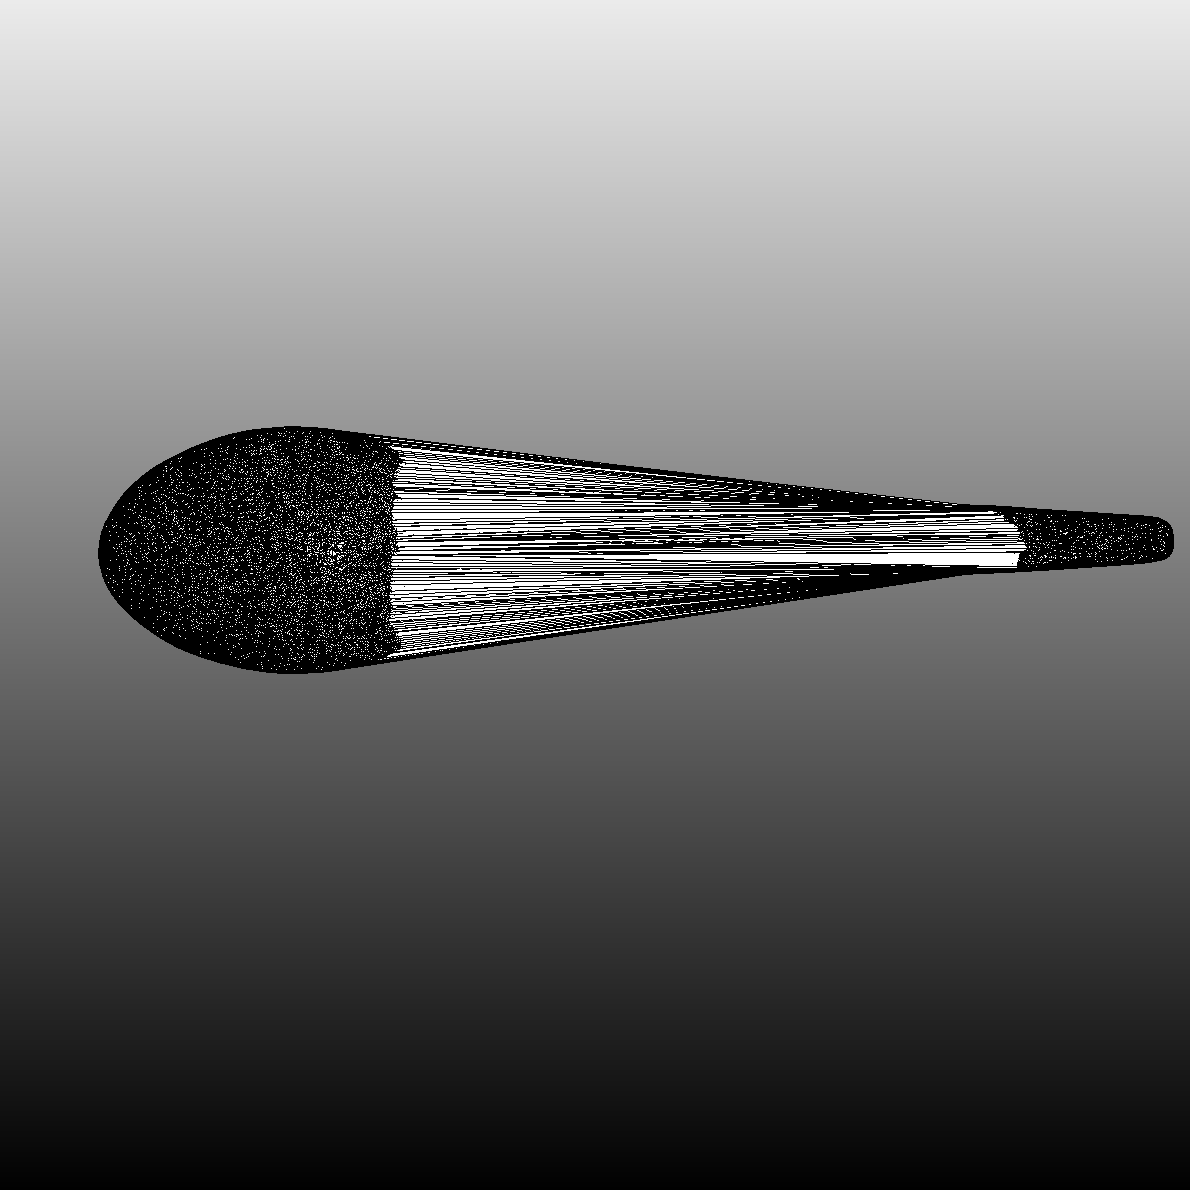
\includegraphics[width=0.22\textwidth]{img/spoon3.png}
    \label{fig:spoonOption3}
  }\hspace{-3mm}
  \subfigure[]{
     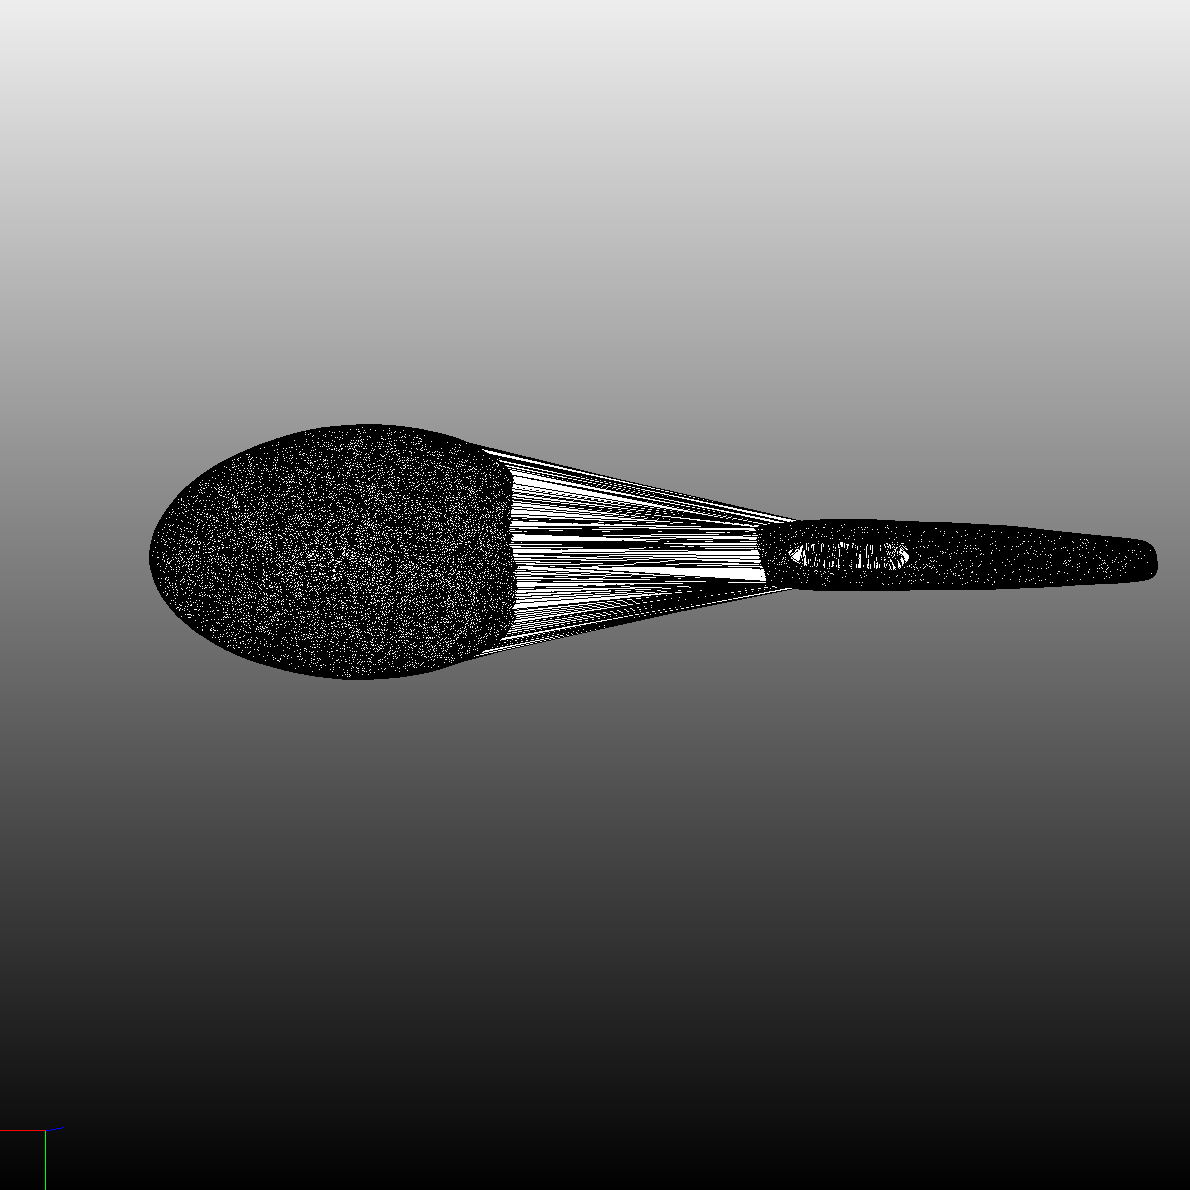
\includegraphics[width=0.22\textwidth]{img/spoon2.png}
     \label{fig:spoonOption2}
  }\hspace{-3mm}
  \subfigure[]{
    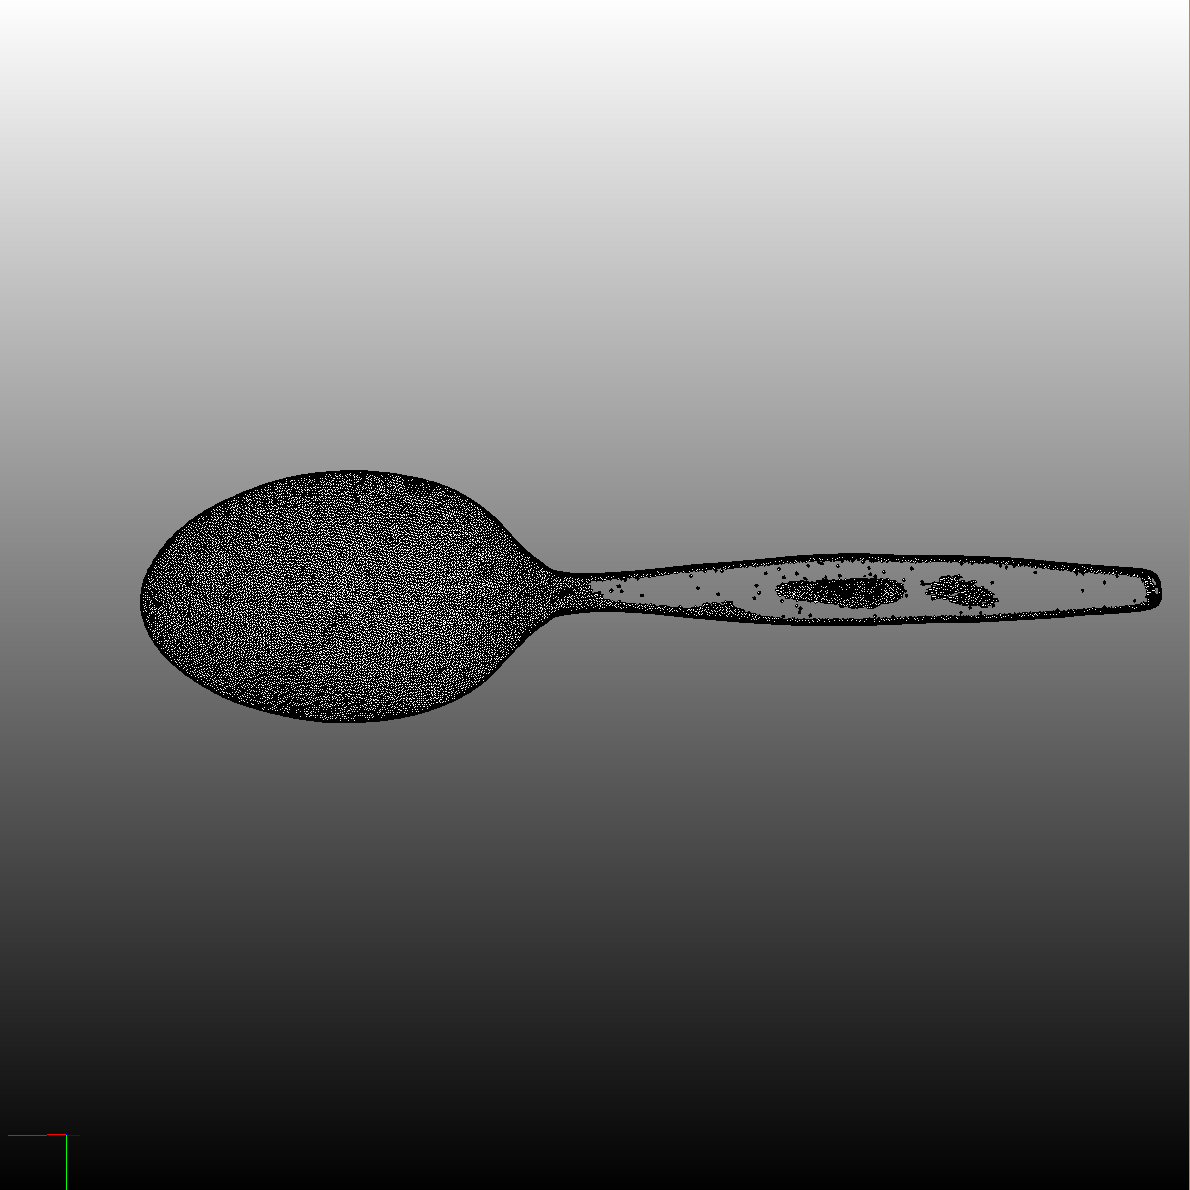
\includegraphics[width=0.22\textwidth]{img/spoon1.png}
     \label{fig:spoonOption1}
  }\hspace{-3mm}
  \subfigure[]{
    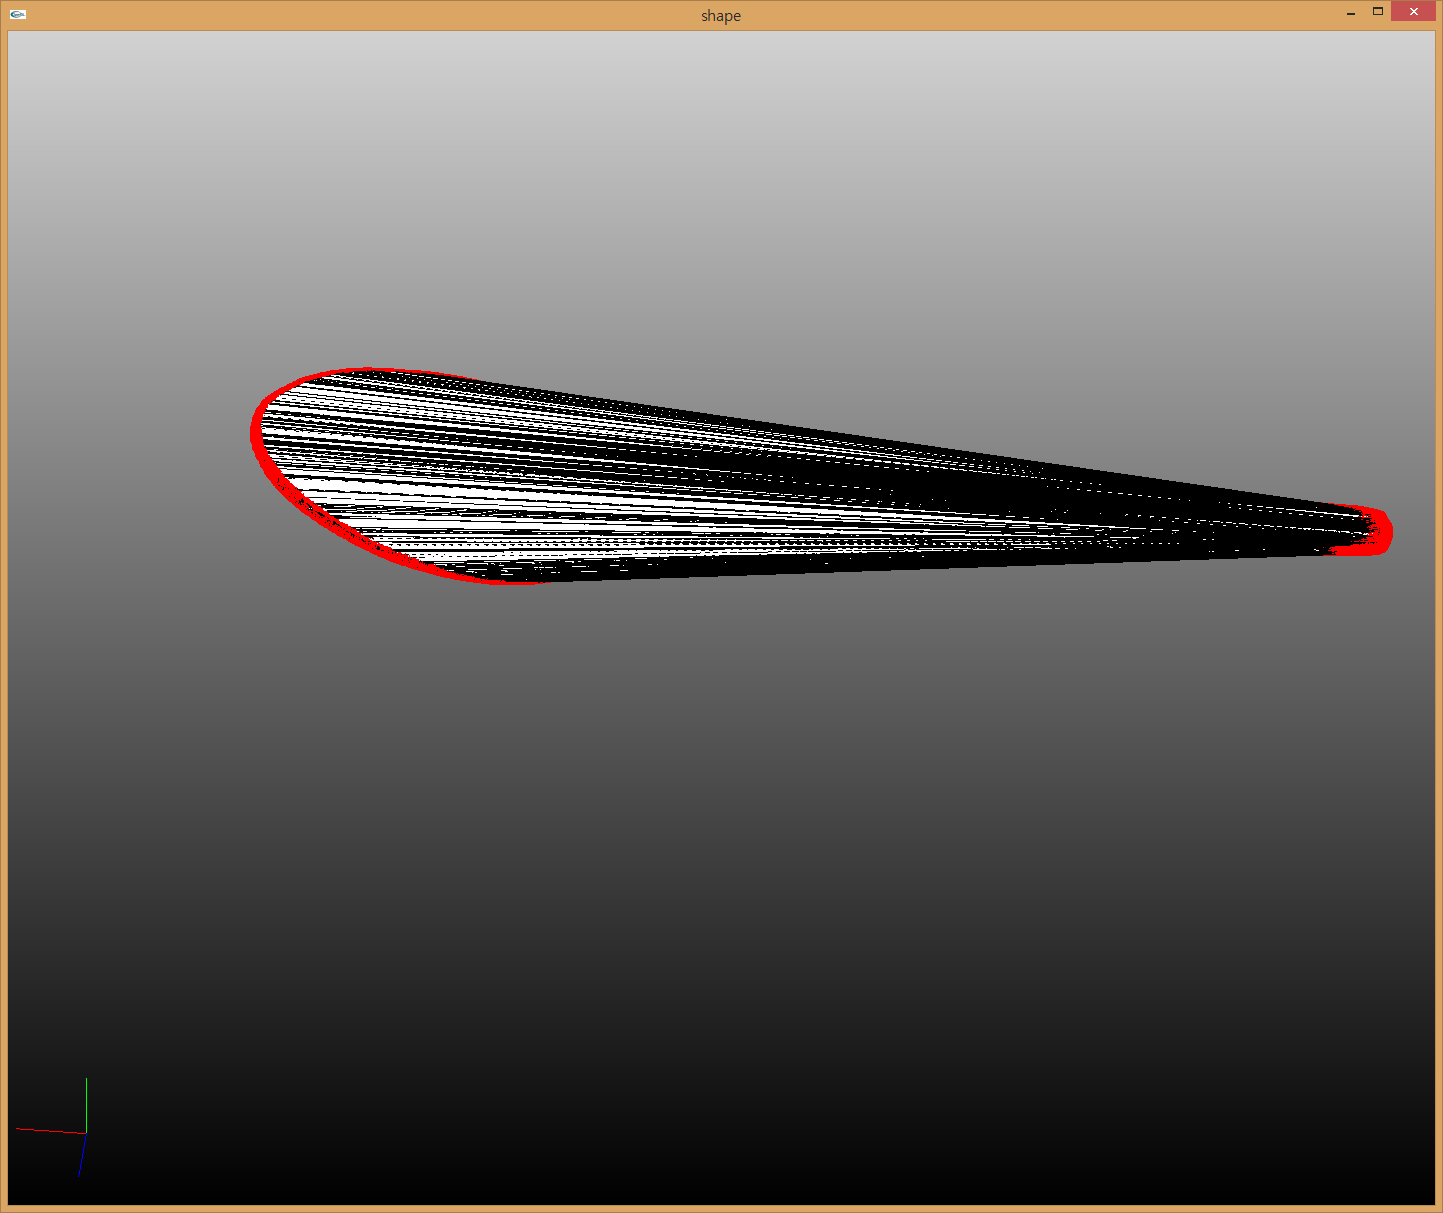
\includegraphics[width=0.22\textwidth]{img/spoon4.png}
     \label{fig:spoonOption4}
  }\hspace{-3mm}
  \caption{A spoon example \label{fig:spoon}}
\end{figure*}
\begin{figure*}[hbt]
 \centering
  \subfigure[]{
    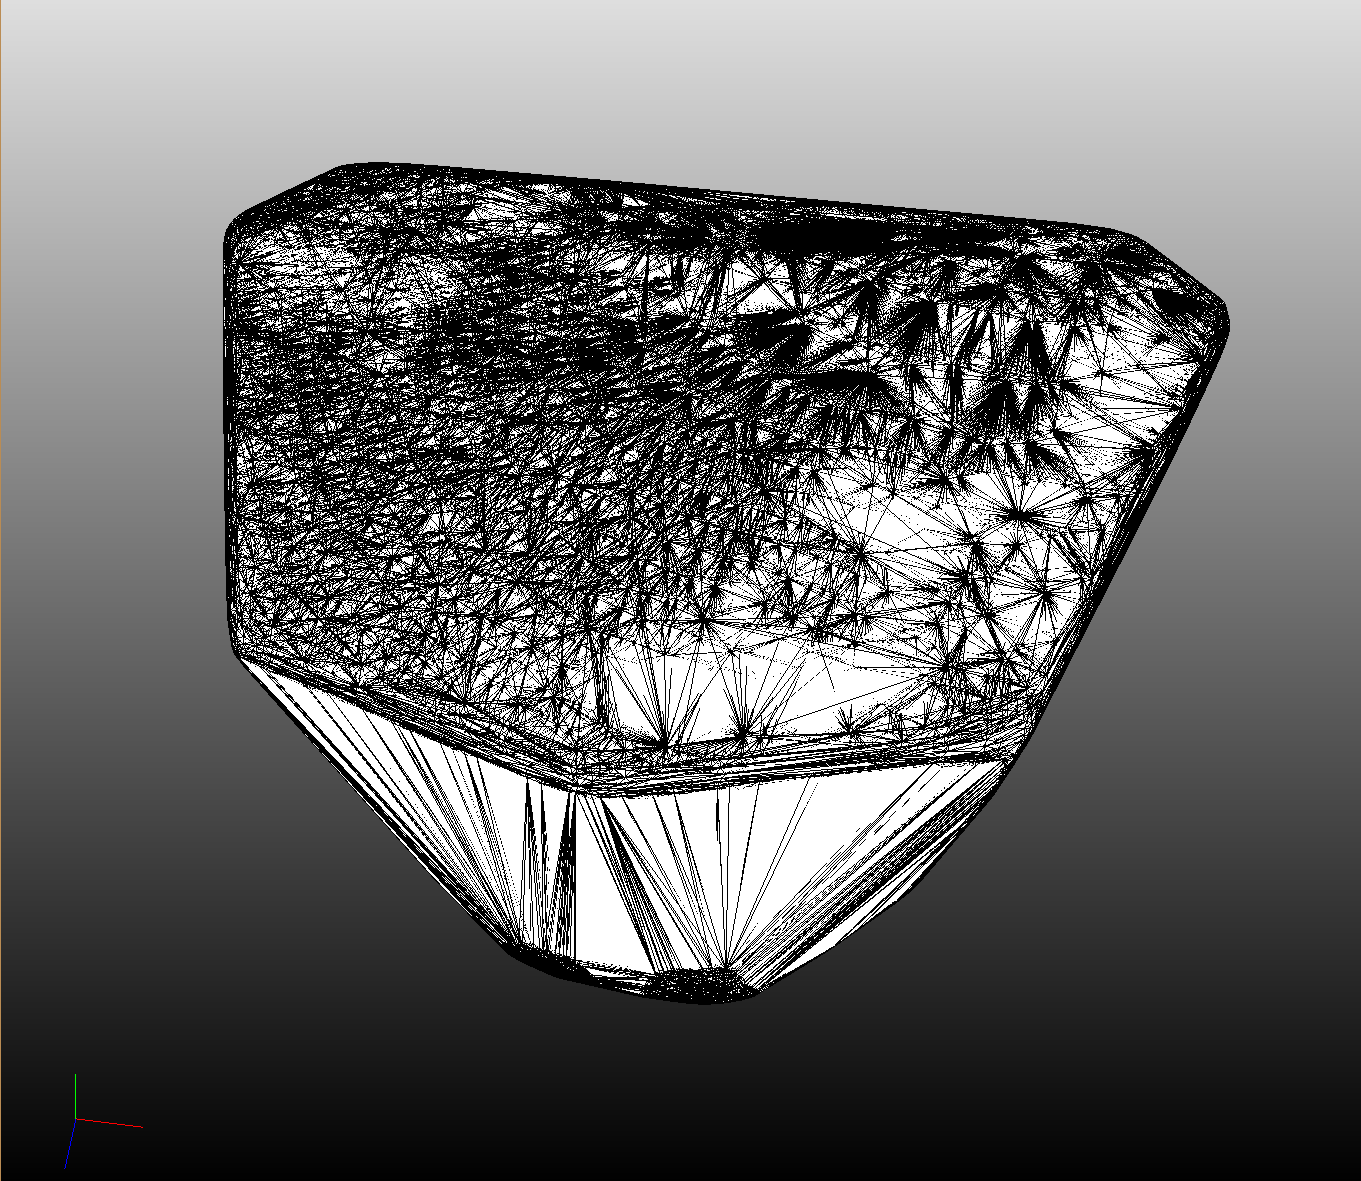
\includegraphics[width=0.22\textwidth]{img/teeth3.png}
    \label{fig:teethOption3}
  }\hspace{-3mm}
  \subfigure[]{
     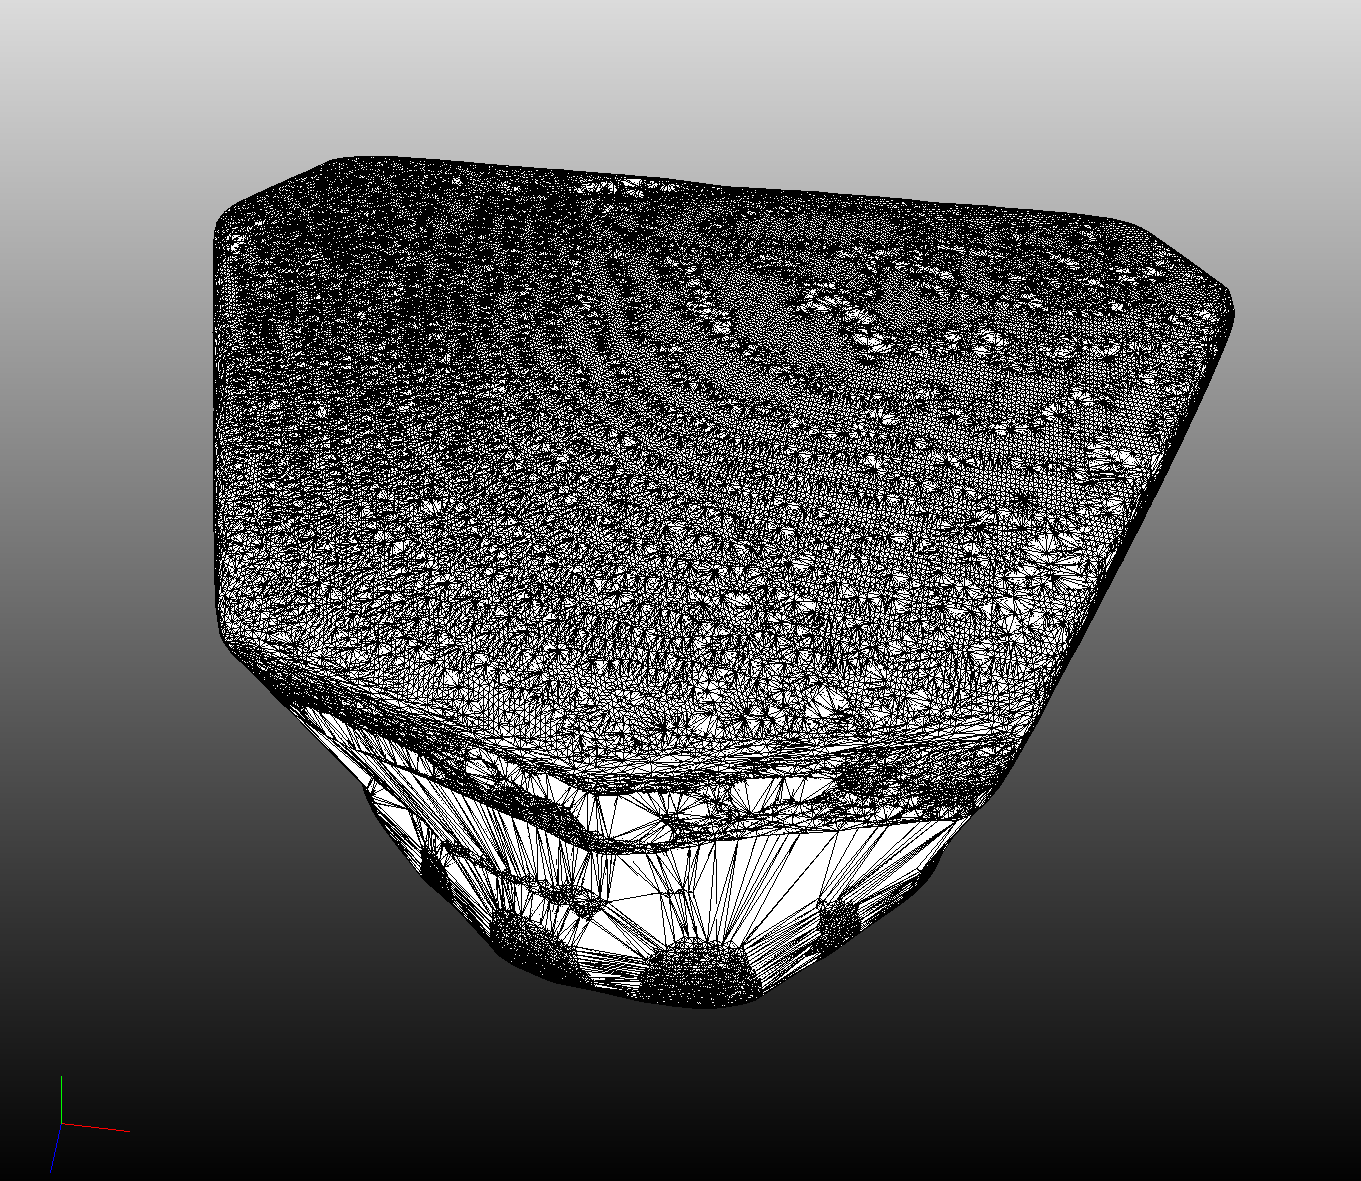
\includegraphics[width=0.22\textwidth]{img/teeth2.png}
     \label{fig:teethOption2}
  }\hspace{-3mm}
  \subfigure[]{
    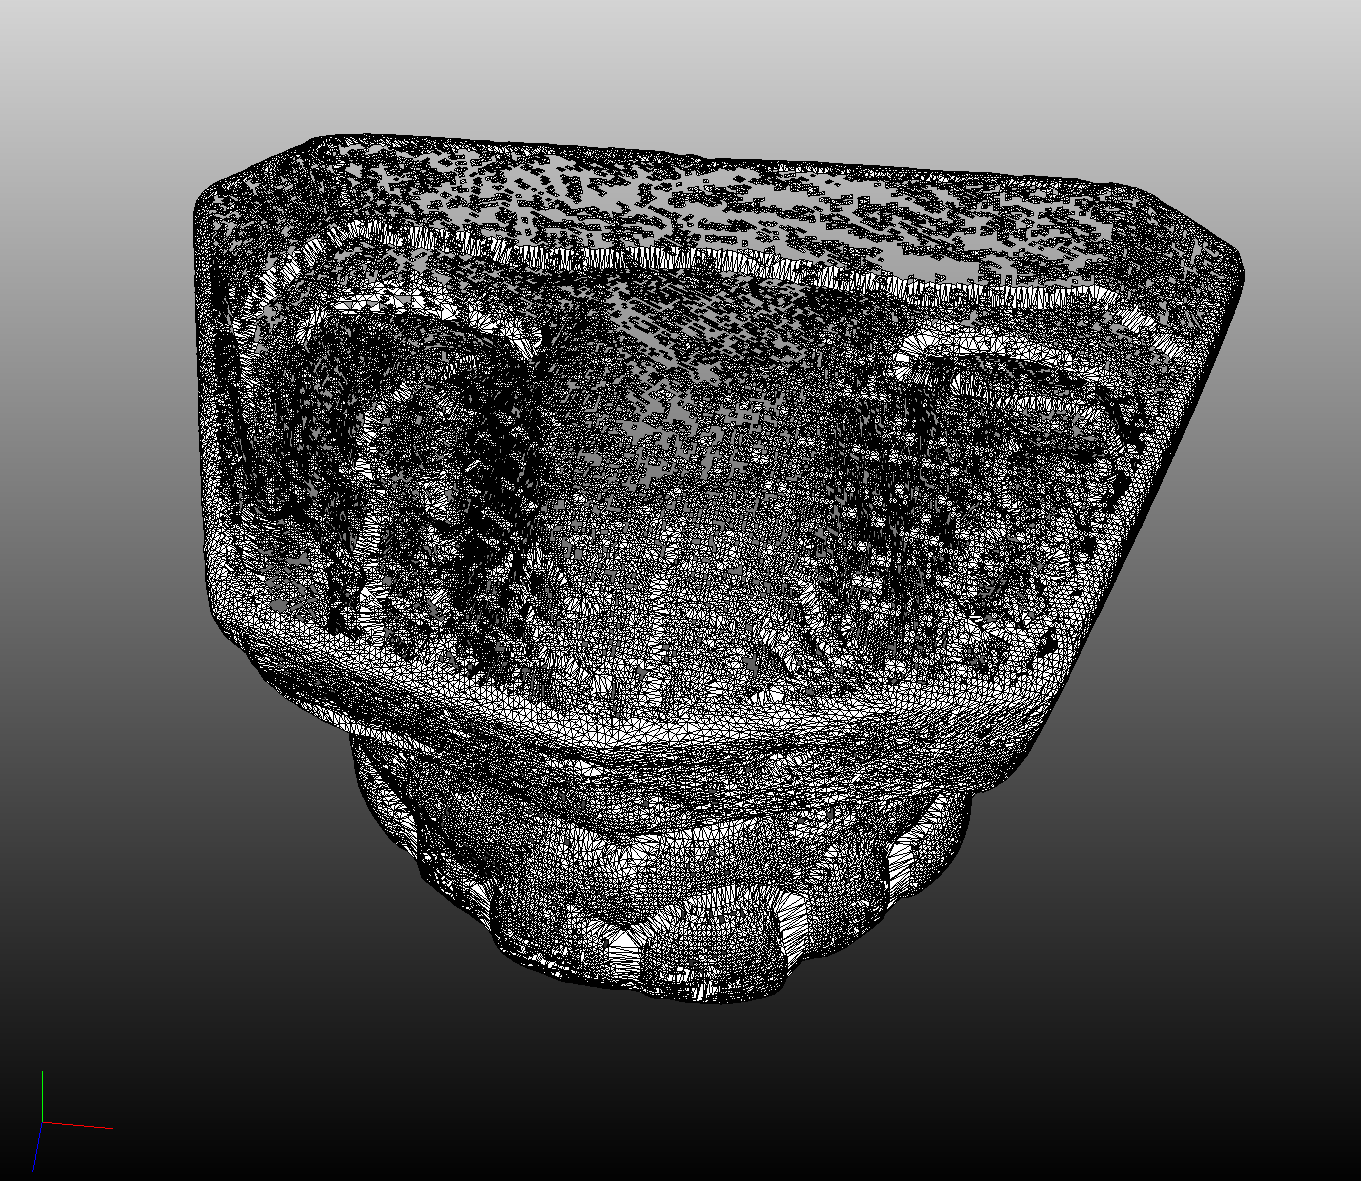
\includegraphics[width=0.22\textwidth]{img/teeth1.png}
     \label{fig:teethOption1}
  }\hspace{-3mm}
  \subfigure[]{
    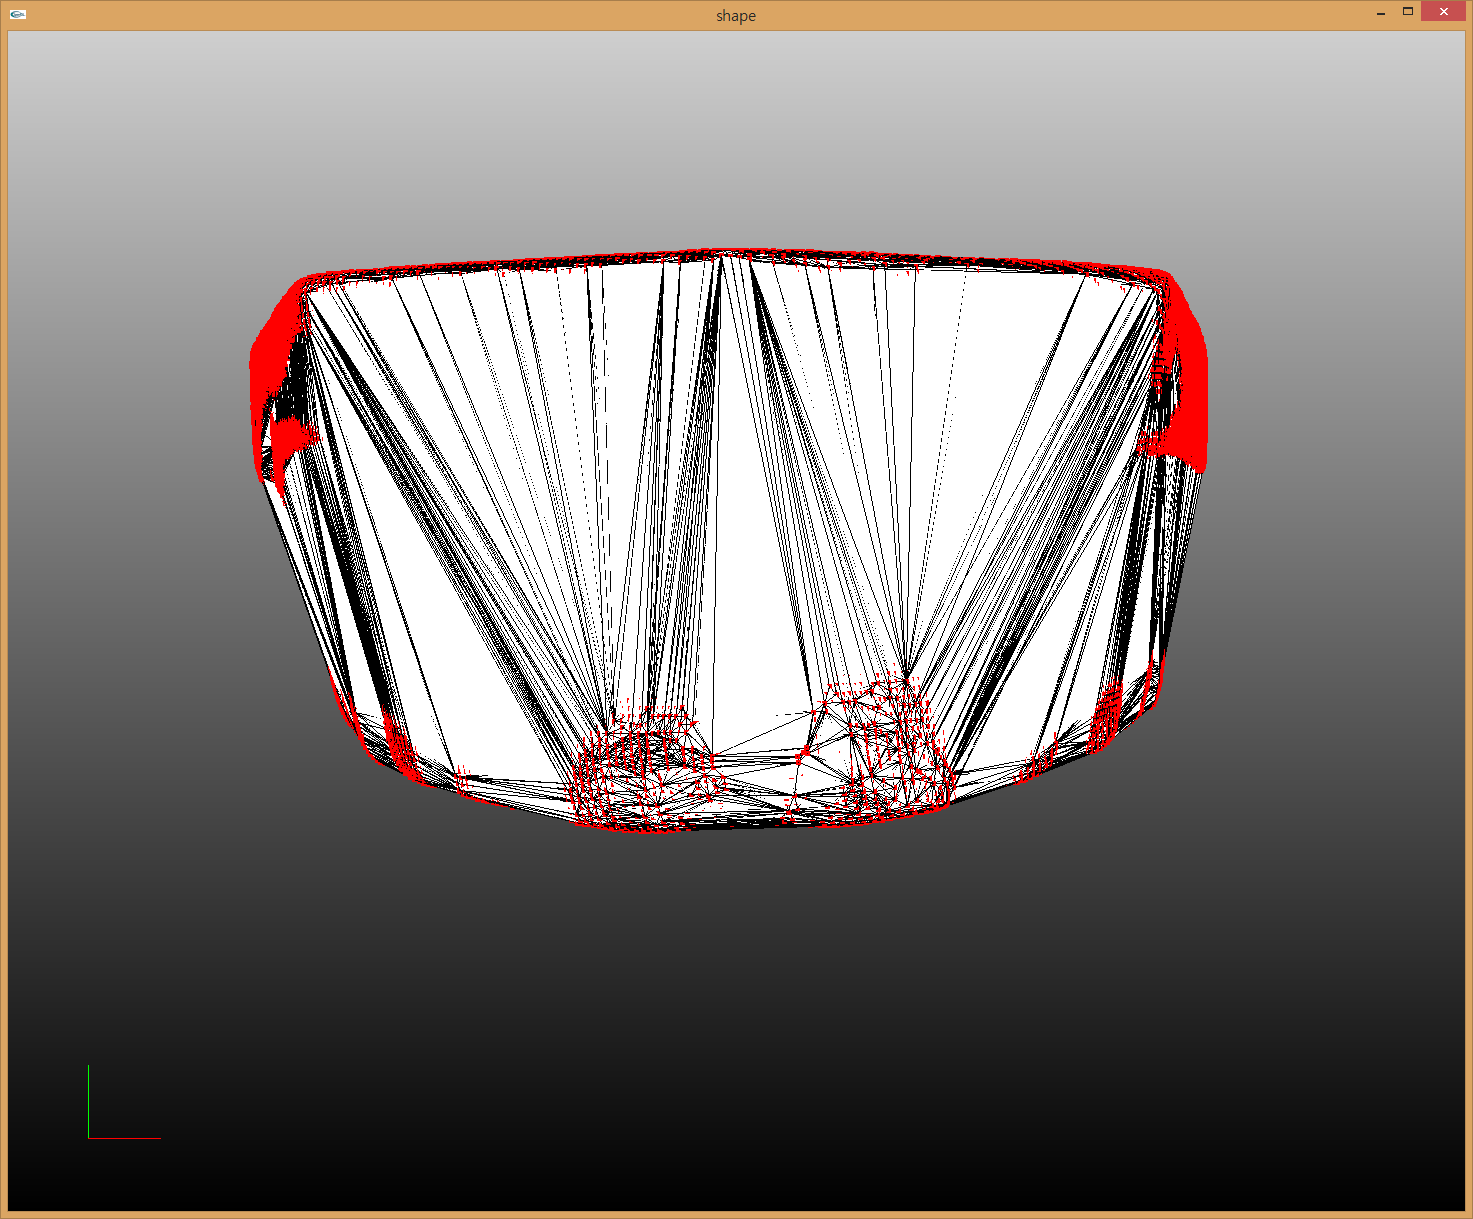
\includegraphics[width=0.22\textwidth]{img/teeth4.png}
     \label{fig:teethOption4}
  }\hspace{-3mm}
  \caption{A teeth example \label{fig:spoon}}
\end{figure*}
\begin{figure*}[hbt]
 \centering
  \subfigure[]{
    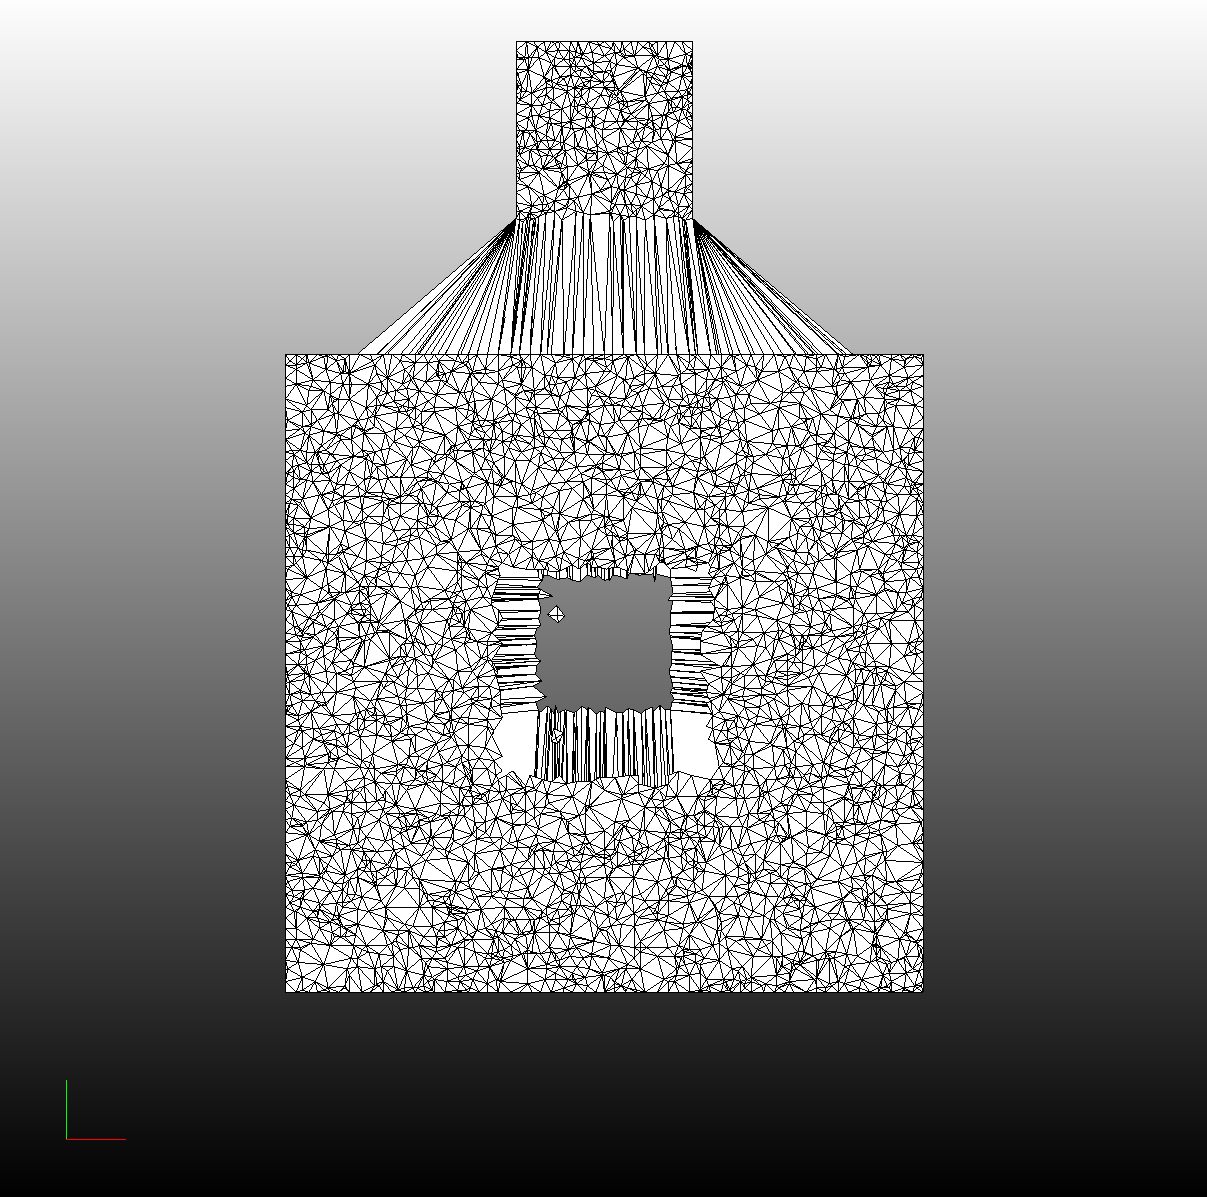
\includegraphics[width=0.42\textwidth]{img/T1.png}
    \label{fig:T1}
  }\hspace{-3mm}
  \subfigure[]{
     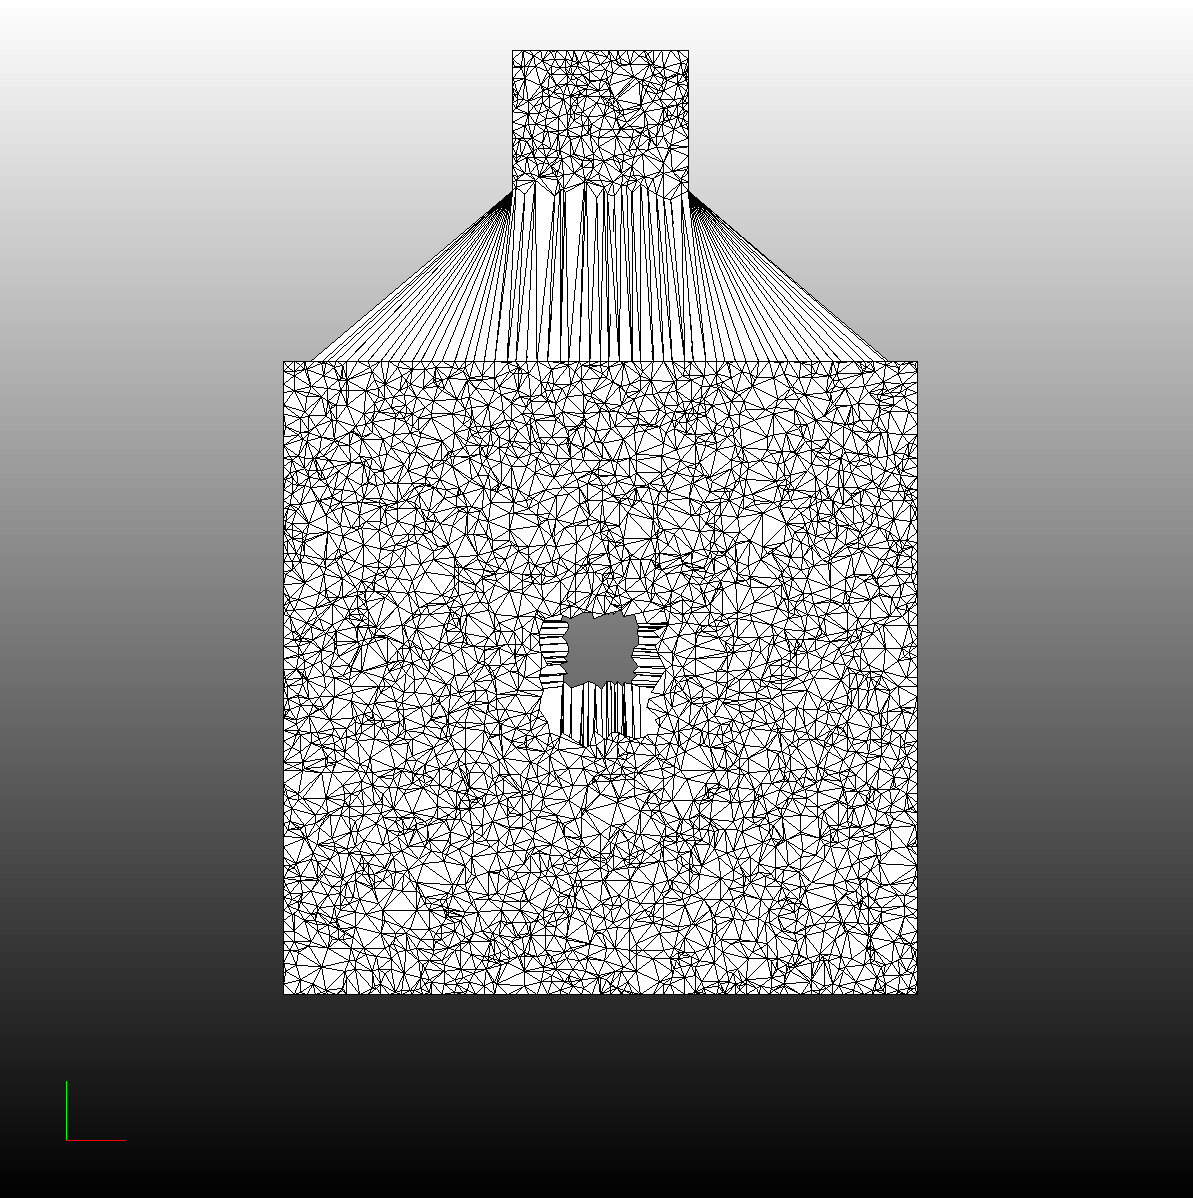
\includegraphics[width=0.42\textwidth]{img/T2.png}
     \label{fig:T2}
  }\hspace{-3mm}
  \caption{Difference between projection result of Delanauy triangulation and all tetrahedra.\label{fig:T}}
\end{figure*}
\section{Know bugs/limitations}
There are some limitations on this code. First, this code doesn't handle the duplication of faces while add tetrahedron to be draw. Also, I found some visual artifact on the Delanauy triangulation of ellipsoid(Fig. \ref{fig:Ellipsoid}). I could not find the reason why.
\begin{figure*}[htb]
  \begin{center}
  \includegraphics[width=0.8\textwidth]{img/ellipsoid1_bug.png}
  \caption{Ellipsoid bug}
  \label{fig:Ellipsoid}
  \end{center}
\end{figure*}

\bibliographystyle{plain}
\bibliography{report}

\end{document}




